%\documentclass[hyperpdf,nobind,draft,oneside]{hepthesis}  %% For normal draft builds, no figs
%\documentclass[hyperpdf,nobind,draft,twoside]{hepthesis}  %% For normal draft builds, no figs
%\documentclass[hyperpdf,nobind,draft,hidefrontback]{hepthesis}  %% For short draft builds
\documentclass[hyperpdf,bindnopdf]{hepthesis}  %%For Cambridge soft-bound version
%\documentclass[hyperpdf,oneside]{hepthesis}  %% For Cambridge hard-bound version

%% Put package includes etc... into a seperate preamble.tex to keep things tidy
%% Contain packages to use, metadata and random tweaks and macros
\usepackage{xspace}
\usepackage{tikz}
\usepackage{mathrsfs}
\usepackage{verbatim}
\usepackage{graphicx}
\usepackage{caption}
\usepackage{subcaption}
\usepackage{url}
\usepackage{hyperref}
\usepackage{lmodern}
\usepackage[english]{babel}
\usepackage[compat=1.1.0]{tikz-feynman}
\usepackage{amsfonts}
\usepackage{mathtools}

\usepackage{amsmath}
\usepackage{cancel}
\usepackage{hepnicenames}
\usepackage{siunitx}
\usepackage[freestanding]{hepunits}
\usepackage{maybemath}
\usepackage{braket}
\usepackage{xspace}
\usepackage{relsize}

\allowdisplaybreaks

\usepackage[style=phys,biblabel=brackets,eprint=true]{biblatex}
\addbibresource{bibliography.bib}

%% Metadata
\makeatletter
\@ifpackageloaded{hyperref}{%
    \hypersetup{%
        pdftitle    = {Convolutional neural networks for the CHIPS neutrino detector R\&D project},
        pdfsubject  = {Josh Tingey's PhD thesis},
        pdfkeywords = {CHIPS, Physics, CNN, Machine Learning},
        pdfauthor   = {\textcopyright\ Josh Chalcraft Tingey}
    }}{}
\makeatother

%% Random tweaks and personal macros
\makeatletter
\g@addto@macro\bfseries\boldmath
\makeatother

\DeclarePairedDelimiter\abs{\lvert}{\rvert}
\DeclarePairedDelimiter\norm{\lVert}{\rVert}

\DeclareRobustCommand{\chips}{\textsc{Chips}\xspace}
\DeclareRobustCommand{\chipsm}{\textsc{Chips-M}\xspace}
\DeclareRobustCommand{\chipsfive}{\textsc{Chips-5}\xspace}
\DeclareRobustCommand{\numi}{NuMI\xspace}
\DeclareRobustCommand{\nova}{NOvA\xspace}

%% You can set the line spacing this way
%\setallspacing{double}
%% or a section at a time like this
%\setfrontmatterspacing{double}

%% Define the thesis title and author
\title{Convolution neural networks for the CHIPS neutrino detector R\&D project}
\author{Josh Chalcraft Tingey}

%% Doc-specific PDF metadata
\makeatletter
\@ifpackageloaded{hyperref}{%
\hypersetup{%
    pdftitle    = {Convolution neural networks for the CHIPS neutrino detector R\&D project},
    pdfsubject  = {Josh Tingey's PhD thesis},
    pdfkeywords = {CHIPS, Physics, CNN, Machine Learning},
    pdfauthor   = {\textcopyright\ Josh Chalcraft Tingey}
}}{}
\makeatother

\begin{document} % Start the document 

\begin{frontmatter}
    %% Contains all the frontmatter such as title page, abstract, declaration and contents etc...
\pagenumbering{arabic}

\title{Convolution neural networks for the CHIPS neutrino detector R\&D project}
\author{Josh Chalcraft Tingey}

\titlepage[University College London]{ %%%%%%%%%%%%%%%%%%%%%%%%%%%%%%%%%%%%%%%%%%%%%%%%%%%%%%%%%%%
    Submitted to University College London in fulfilment of the \\
    requirements for the award of the degree of \textbf{Doctor of Philosophy}
}
\thispagestyle{plain}

\begin{declaration} %%%%%%%%%%%%%%%%%%%%%%%%%%%%%%%%%%%%%%%%%%%%%%%%%%%%%%%%%%%%%%%%%%%%%%%%%%%%%%
    I, Josh Chalcraft Tingey confirm that the work presented in this thesis is my own. Where
    information has been derived from other sources, I confirm that this has been indicated in the
    thesis.
    \vspace*{1cm}
    \begin{flushright}
        Josh Tingey
    \end{flushright}
\end{declaration}

\begin{abstract} %%%%%%%%%%%%%%%%%%%%%%%%%%%%%%%%%%%%%%%%%%%%%%%%%%%%%%%%%%%%%%%%%%%%%%%%%%%%%%%%%
    This is an abstract
\end{abstract}

\chapter*{\centering Impact statement}
This is an impact statement

\begin{acknowledgements} %%%%%%%%%%%%%%%%%%%%%%%%%%%%%%%%%%%%%%%%%%%%%%%%%%%%%%%%%%%%%%%%%%%%%%%%%
    These are some acknowledgements
\end{acknowledgements}

\tableofcontents %%%%%%%%%%%%%%%%%%%%%%%%%%%%%%%%%%%%%%%%%%%%%%%%%%%%%%%%%%%%%%%%%%%%%%%%%%%%%%%%%
\listoffigures %%%%%%%%%%%%%%%%%%%%%%%%%%%%%%%%%%%%%%%%%%%%%%%%%%%%%%%%%%%%%%%%%%%%%%%%%%%%%%%%%%%
\listoftables %%%%%%%%%%%%%%%%%%%%%%%%%%%%%%%%%%%%%%%%%%%%%%%%%%%%%%%%%%%%%%%%%%%%%%%%%%%%%%%%%%%%
\end{frontmatter}

\begin{mainmatter}
    \chapter{Introduction}
\label{chap:introduction}

%% Restart the numbering to make sure that this is definitely page #1!
\pagenumbering{arabic}

\begin{comment}
TODO: Write the story of the introduction chapter

TODO: Write the introduction chapter section outline

TODO: Add all the sections below
\end{comment}
    \chapter{Neutrino oscillations: theoretical background and current status}
\label{chap:theory}

Consider a simple two body decay
Neutrino physics covers the widest possible range of
Proposal of a mysterious undetector particle to explain beta decays in the 1930s through to the resolutions of a 30-year problem with the confirmation of oscillations in the early 2000s and onto the precision era.
Neutrino oscillations first discoveed in 1957 when Bruno Pornecorvo proposed a model in which neutrinos oscilate to antineutrinos and back, similar to the kain. It was actually shown that neutrinos iscilate from one flavour to another.
The field of neutrino physics is ever expanding with a new generation of experiments planned for the coming years.
This chapter aims to provide an introduction to neutrino

\section{A history of neutrino oscillations}
\label{sec:theoryhistory}

\begin{comment}
TODO: Maybe add a few diagrams of the key plots throughout history
\end{comment}

In the early 20th century, beta decays were assumed to follow the simple two-body process, $A \rightarrow B + e$, where a
nuclei spontaneously an electron, and only an electron. To conserve both energy and angular momentum the ejected electron
must have a discrete kinetic energy defined by the difference in binding energies between the initial and final nuclei.
However, in 1914, J. Chadwick instead measured a continuous energy spectrum for the electron ~\cite{chadwick1914},
placing this theory in doubt.

W. Pauli finally proposed a 'desperate solution' to this paradox in 1930 ~\cite{pauli1930}. If a light, neutrally charged,
spin $1/2$ particle was also produced in the interaction, the continuous energy distribution could be explained. Initially
this mysterious new particle was named the 'neutron'. But, to avoid confusion with the heavy baryon of the same name discovered
in 1932, E. Fermi renamed it the 'neutrino' when he formalised beta decay in 1934 ~\cite{fermi1934}.

The following month, H. Bethe and R. Peierls used Fermi's work to estimate the cross-section of the inverse beta decay process
${\nu} + p^{+} \rightarrow n + e^{+}$ ~\cite{bethe1934}. They calculated a value of less than the very small $10^{-44} cm^2$
and declared 'there is no practically possible way of observing the neutrino.' Although extensive neutrino detection has
proved possible, it hinted at the huge difficulties experimentalists would face hunting down the neutrino and measuring
it's properties in the years to come.

After an initial tentative identification if 1953, F. Reines and C. Cowan made the first confirmed observation of the neutrino
in 1956 ~\cite{cowan1956}. Electron antineutrinos produced in the Savannah River Plan nuclear reactor were detected via the
inverse decay process outlined in the previous paragraph. A 'club-sandwich' detector of three 1500 litre liquid scintillator tanks
and two 200 litre cadmium doped water target tanks, was constructed in an underground room of the reactor building. A total of
330 photomultiplier tubes were then able to measure the prompt positron annihilation signal followed by the gamma ray burst from
the neutron capture in cadmium, the signature identification for the interaction.


Brookhaven two kinds of neutrinos in Ref.~\cite{danby1962}
- Muon neutrino discovered by the 'long track' from the decays of pions from a reactor in 1988, got a nobel prize.
- In 1962 at the alternating gradient synchrotron at Brookhaven, neutrinos created from pion decays together with muons were observed t produce only muons not electrons, this then confirmed the existence of the muon neutrino.
- Neutrinos originating from pion decays primary produce muons, not electron. Detected as single long tracks in a spark chamber.
- Got the 1988 nobel prize for this discovery of the second neutrino.
- Distinct from the previously known electron neutrino
- The neutrinos produced by the pions decay from a accelerator beam, were not the same as the neutrinos observed in beta decay
- Did so by observing that it was far more likely that the neutrinos pro-duced in the decay of pions would interact to create muons, as opposed to electron
- First experiment to construct and use an artificial neutrino beam
%- νμ+p+→μ++n and ̄νμ+p+→e++n with a single neutrino would be expected to happen at the same rate, only muons were produced.
- 34 identified muon events in total no electrons.


Discovery of the tau lepton ~\cite{perl1975}
Also precise z-resonance measurement at lep in the 1990's ~\cite{electroweak2006}
Finally measured by DONUT in 2000 ~\cite{Kodama2001}
- evidence for the third neutrino, finally discovered at DONUT in 2000
- After the discovery of the tau lepton in 1975 ~\cite{perl1975}, this suggested the existence of the third neutrino which DONUT found in 2000.
- DONUT finally found the tau neutrino in 2000 using 800GeV protons from the Tevatron.
- In 2000 the DONUT experiment at the tevatron collider in fermilab performned a direct detection of the tau neutrino completing the three flavour picture.
- Experiments at the LEP e+e- collider in the 1990s made precision measurmnets of the z decay width, from a fir to the data in showed there are exactly three active generations of neutrinos.
- This indicates the number of active neutrino states can only be 1.984+-0.008. Therefore, any as yet undiscovered neutrinos must be sterile, in that they do not couple to the weak interaction.
%- Hence, all flavours of neutrino had been found, but the strongest constraint is due to the width of the Z^0 resonance. 


Homestake deficit observation in Ref.~\cite{davis1968}
first SSU predictions used to compare against homestake in Ref.~\cite{bahcall1968}
Kamiokande II deficit in Ref.~\cite{hirata1989}
SAGE experiment deficit in Ref.~\cite{abazov1991}
GALLEX experiment deficit in Ref.~\cite{anselmann1994}
SSM Prediction for Ga in Ref.~\cite{bahcall1988}
- As the standard model of particle physics was developed, neutrinos were presumed to be massless and occur only in the three flavour eigenstates.
- Various hints that this was not the case kept appearing, leading to neutrino oscillations, by witch one neutrino can oscillate to another flavour and the non-zero masses that follow as a direct consiquence from this.
- In the solar neutrino sector there is the "solar anomaly" noting a deficit of electron neutrino compared to predications made by the standard solar model (SSM)
- First observed at the Homestack experiment, neutrinos ineracted with the chlorine creating radioactive argon atoms, beause it is a noble gas it does not bing to the perchloroethylene and it can be extracted by purging the liquid with gaseous helium and then extracted from the helium with a cooled carbon trap.
- Gallium was also used by other experiments and kamiokande also observed the deficit.
- Also the fluxes measured where not consistent, depending on the energy range probed. Hinting at oscillations dependent on energy,
%- 4p+ 2e−→4He + 2νe+ 26.73MeV−Eν pp-chain in the sun whereEνis the energy of the two neutrinos, and (26.73 MeV -Eν) is the energyemitted as photons
%- νe+37Cl→37Ar +e−(threshold 814 keV) in homestake, periodically flushed with helium
- 400 000 litresof perchloroethylene (a dry-cleaning fluid), containing520 tof chlorine, placed in the Homestake Mine,1.5 kmunderground [24].
%- chlorine solution capable of neutrino capture(νe+37Cl→37Ar + e−).  The atoms of argon were counted and used as a measure of the neutrinoflux.
- he reported experimental rate was about two thirds less than what was expected from theStandard Solar Model (SSM). This large discrepancy, known as thesolar  neutrino  problem, wasinitially believed to be an experimental flaw.
% ν+Ga71→Ge71+e− for sage and gallex
- This is where the future DUNE detector will be housed, nice full circle
- This is in the solar sector

SNO oscillation measurement in Ref.~\cite{ahmad2002}
- neutrino oscillations were one way of explaining this deficit if some of the electron neutrinos converted flavour in flight.
- SNO finally answered the question when it was able to measure three channels with different relation between te flyx or electron neutrinos and the other neutrinos. SNO could prove that the electron neutrinos are changing flavour. WHile the total flux of all neutrinos remains constant and in agrrement with the SSM.
- 1kton tank of heavy (D2O deuterium) water, able to detect three different channels of neutrino interaction
%- νe+d→p+p+e− νx+d→p+n+νx νx+e−→νx+e−
- Cherenkov experiment, with 9500 8inch photomultiplier tubes detectro the light from neutrino interactions.
- Since each of the rates for the three channels has a different relation between the flux of electron neutrinos and the others, SNO could confirm electron neutrinos are changing flavour, with the total flux being constant and in agreement with the SSM.
- electron neutrino CC, NC and elastic scattering also.
- total rate was consistent but less electron neutrinos than expected as they had oscillated.
- However, only electron neutrinos canundergo CC interactions, as solar neutrinos do not have enough energy to produce muonor tau leptons.
- %e+d→p+p+e−(CC) νx+d→p+n+νx(NC) νx+e−→νx+e−(ES) The CC channel is sensitive exclusively to electron neutrinos, whilst the other two are acces-sible by neutrinos of any flavour. 

Atmospheric kamiokande deficit in Ref.~\cite{hirata1988}
IMD detector atmospheric deficit in Ref.~\cite{becker1992}
Superkamiokande direction atmospheric neutrinos in Ref.~\cite{becker1992}
- This is in the atmospheric sector

\section{Neutrino oscillation theory}
\label{sec:theorytheory}

blah blah blah

\section{Current status and the future}
\label{sec:theorystatus}

\subsection{Atmospheric}

\subsection{Accelerator experiments}

\subsection{Reactor experiments}

\subsection{The future}


blah blah blah
    \chapter{Long baseline water Cherenkov detectors} %%%%%%%%%%%%%%%%%%%%%%%%%%%%%%%%%%%%%%%%%%%%%%%%
\label{chap:exp} %%%%%%%%%%%%%%%%%%%%%%%%%%%%%%%%%%%%%%%%%%%%%%%%%%%%%%%%%%%%%%%%%%%%%%%%%%%%%%%%%

\begin{comment} % PLAN %%%%%%%%%%%%%%%%%%%%%%%%%%%%%%%%%%%%%%%%%%%%%%%%%%%%%%%%%%%%%%%%%%%%%%%%%%%
TODO: Write the story of the exp chapter

TODO: Write the exp chapter section outline

NEUTRINO INTERACTIONS
- Feynman diagrams of all the main interaction types
- Famous diagrams of cross-section regions for them all
- Descriptions of which types are easy to detect, what are the main NC backgrounds usually etc...

\end{comment}

- Say how they are usually very expensive due to volume required
- Large overburden/excavation costs etc...
- Beam
- cherenkov light
- PMTs
- water clarity
- overburden
- interaction types (which ones are the problem)
- What they are good at, what they are bad At
- Historical WC detectors

\section{Neutrino interactions} %%%%%%%%%%%%%%%%%%%%%%%%%%%%%%%%%%%%%%%%%%%%%%%%%%%%%%%%%%%%%%%%%%
\label{sec:exp_interactions} %%%%%%%%%%%%%%%%%%%%%%%%%%%%%%%%%%%%%%%%%%%%%%%%%%%%%%%%%%%%%%%%%%%%%

\begin{figure} % CROSS-SECTION DIAGRAM %
    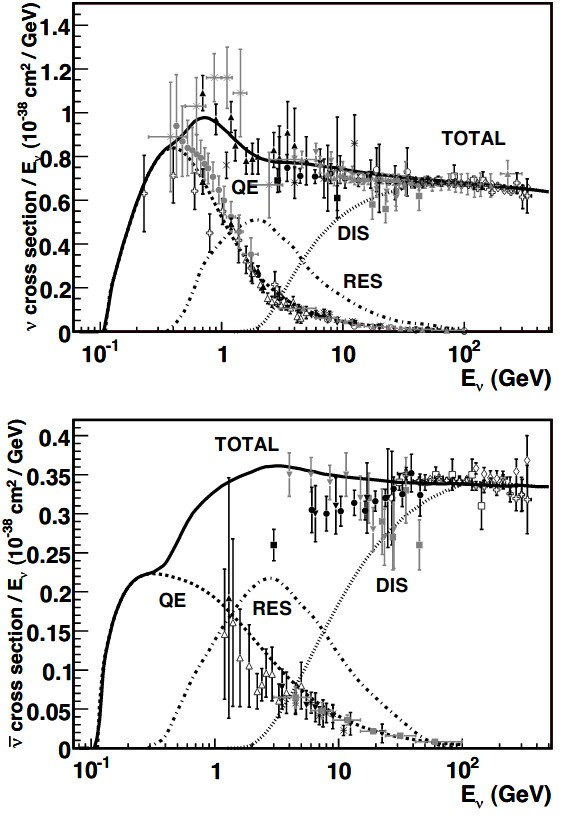
\includegraphics[origin=c,width=0.6\textwidth]{diagrams/4-exp/cross_sections.png}
    \caption[cross sections short]
    {Figure taken from Ref.\cite{formaggio2012}.}
    \label{fig:cross_sections}
\end{figure}

\begin{figure} % TAU CROSS-SECTION DIAGRAM %
    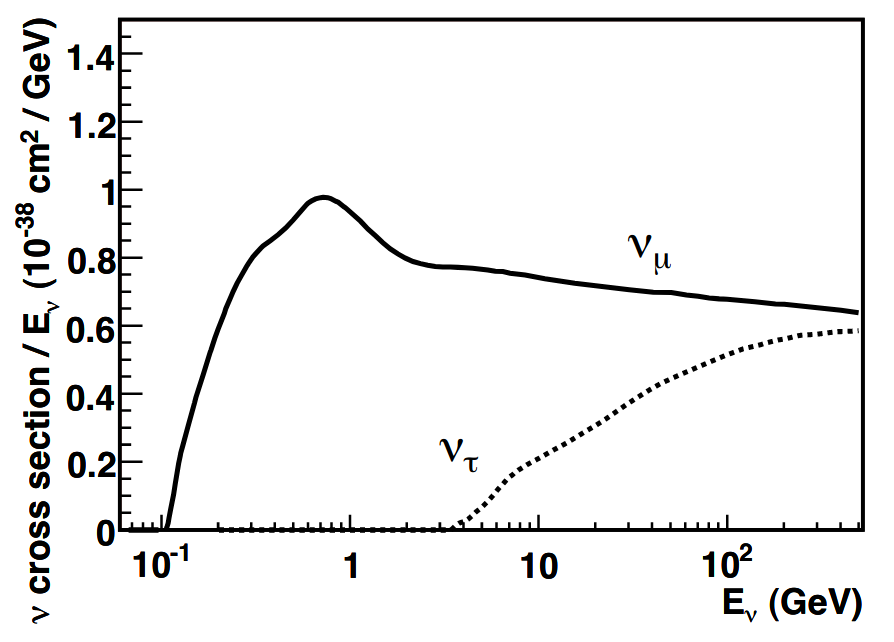
\includegraphics[origin=c,width=0.6\textwidth]{diagrams/4-exp/tau_comparison.png}
    \caption[tau comparison short]
    {Figure taken from Ref.\cite{formaggio2012}.}
    \label{fig:tau_comparison}
\end{figure}

\begin{figure} % FEYNMAN INTERACTION TYPE DIAGRAMS %
    \feynmandiagram[horizontal=a to b] {
    i1 [particle=\(e^{-}\)] -- [fermion] a -- [fermion] i2 [particle=\(e^{+}\)],
    a -- [photon, edge label=\(\gamma\), momentum'=\(k\)] b,
    f1 [particle=\(\mu^{+}\)] -- [fermion] b -- [fermion] f2 [particle=\(\mu^{-}\)],
    };
    \feynmandiagram[horizontal=a to b] {
    i1 [particle=\(e^{-}\)] -- [fermion] a -- [fermion] i2 [particle=\(e^{+}\)],
    a -- [photon, edge label=\(\gamma\), momentum'=\(k\)] b,
    f1 [particle=\(\mu^{+}\)] -- [fermion] b -- [fermion] f2 [particle=\(\mu^{-}\)],
    };
\end{figure}

- From eV to EeV: Neutrino Cross-Sections Across Energy Scales
- Neutrino originally postulated by Wolfgang Pauli in 1930, and has played a prominent role in
understanding of nuclear and particle physics.
- The revalation that neutrinos can no longer be massless is perhaps the first significant
alteration to the standard model.
- A nice plot of neutrino energy regimes from Big Bang through accelerator to Extra-galactic vs
their cross-sections. I could definitely use this and cite it to the paper
- Contains a good description of fundamental electroweak scattering if we need a reference for
that (page 4->)
- First anumu + e- => anumu + e- scattering made by CERN bubble cchamber experiment Gargamelle
- This and DIS NC observations confirmed the weak neutral currents and helped solidify the
standard model.
- Maybe include a bubble chamber image of the first candidate neutrino interaction.
- At intermediate energy scales (CHIPS range) interactions fall into three main catageories.
Elastic and quasi-elastic scattering, resonance production and DIS.
- Include an actual data cross-section plot for both CC and NC showing contributions from
different experiments
- Show the tau-neutrino cross section compared to the muon/electron in our energy range to show it
doesn't matter. All the interactions and arguments that go along with them are the same for
nuel/numu as with nutau, except for one key difference; the energy threshold. The nutau
interaction CC cross section is severely altered because of the large tau lepton mass. Then
show the plot.
- Bellow 2Gev it's mainly quasi-elastic with the neutrino scattering of the entire nucelon, rather
than its consituent partons.
- Modern experiments MiniBooNE and NOMAD see higher absolute cross-sections than expected. It is
currently believed that nucelear effects beyond the impulse approximation are desponsible for the
discrepancy. Such as nucleon-nucleon correlations and two-body exchange currents must be included
to get it righ. THIS IS MEC!
- NC QEL lots of people call NC Elastic Scattering, the ratio of NC Elastic/CC QE is ~0.11 from
measurements by a few experiments.
- Single pion production is when the neutrino excites the struck nucleon producing a baryon
resonance, which then quickly decays most often into a nucleon and a single pion final state.
There are seven possible single pion channels, 3CC and 4NC, which we see from the GENIE events.
- Show all the interaction equations for these %νμp→μ−pπ+ etc...
- NC pi-zero production is often the largest numu-induced backgrond in experiments searching for
numu->nuel oscillations. And CC pi production can present a non-negligable complication in the
determination of neutrino energy in experiments. Therefore measuring and modelling nuclear effects
in pion production has become paramount.
- These resonances can also decay into photons with a small branchng fraction, yes, but, like NC
pi-zero production they still pose a non-negliable source of background to the CHIPS main search.
- Neutrinos can also coherently produce single pion final state. In this case the neutrino
coherently scatters from the entire nucleus transferring negligable energy to the target. Hence,
you produce a ditinctly forward-scattered pion with no nuclear recoil. This process is relatively
small however.
- The resonances can also decay to multi-pion final state, along with DIS this contributes a
copious source of multi-pion final states. However, due to the inherant complexity of
reconstructing multiple pion final states, not many experiments look at these cross-sections.
- You can also get kaon production but they have small cross-sections due to the kain mass and
because kaon channels are not enhanced by any dominant resonance.
- You then get DIS where the neutrino scatters of a quark in the nucleon via the exchange of a
virtual W or Z boson producing a lepton and a hadronic system in the final state.
- To isolate DOS events experiments typically apply kinematic cuts to remove QE scattering and
resonance-mediated contributions from their data.

\subsection{Future experiments} %%%%%%%%%%%%%%%%%%%%%%%%%%%%%%%%%%%%%%%%%%%%%%%%%%%%%%%%%%%%%%%%%%
\label{sec:exp_future} %%%%%%%%%%%%%%%%%%%%%%%%%%%%%%%%%%%%%%%%%%%%%%%%%%%%%%%%%%%%%%%%%%%%%%%%%%%

Daya bay theta13 Ref.~\cite{an2012}
RENO theta13 Ref.~\cite{ahn2012}
Double Chooz theta13 Ref.~\cite{abe2012}

- With the measurements of a non-zero theta13 by reactor neutrino experiments, the main focus now
has shifted to resolving the mass hierarchy ambiguity and measuring delta-cp. These can be probed
by long-baseline neutrino experiments by looking to numu to nuel transitions.
- BIG EQUATION FOR PROBABILITY: shows sensitivity to the mass hiearchy through the matter effect
parameters A and to the cp-violtating phase trhough the second term.
- Over that last 20 years neutrino oscillations have become well-established and we are now moving
into the precision measurement era.
- DUNE is a next-generation neutrino oscillation experiment with a primary scientific goal of
observation of CP-violation in the neutrino sector.
- In DUNE a muon neutrino(anti-neutrino) beam will be produced by the Long-Baseline Neutrino
Facility (LBNF)
- There will be a near detector at Fermilab before the neutrinos travel the 1285km to the Sanford
Underground Research Facility (SURF) in South Dakota.
- The far detector will consist of four 10kt (fiducial) liquid argon time projections chamber
(LArTPC) detectors.
- Neutrino oscillation probabilities can then be infered by comparisons of the observed neutrino
spectra and the near and far detectors.
- Recent obsevation of a large theta13 have focuseed the next genetation of long baseline
experiments towards the mass hierarchy, octant of theta23 and measureing delta-CP
- Nova and T2k will not be able to measure the remaining unknows (check this)
- Dune will hopefully solve these problems but will be increadibly expensive

- Symmetries under charge-conjugation and parity inversion are both macimally violated by the
waek interaction.
- Their combined operation has been shown to be violated, to a small degress, by quark mixing
processes.
- If sin(delta-cp) is non zero then vacuum oscillation properties of nu and anti nu will be
different.
- DUNE (I assume CHIPS) is sensative to four oscillation paramters, delta31, theta23, theta13
and delta-cp.
- These can be measured using four data sample, two for neutrino and two for antineutrinos.
- These sample are produced by "Forward Horn current" FHC and "Reverse Horn current" RHC,
producing predominetetly neutrinos and anti-neutrinos respectively.
- Dissapearence channels sensitive to %abs(delta31^2), and sin^2(2theta23).
- Apperence channels sensitive to all four parameters including sign of %delta32^2.
- The "signal" in all cases are CC interactions, therefore selection of nuel, anuel, numu and
anumu CC is the goal.
- Main background in CC numu selections are NC with charged pions.
- Main background in CC nuel selections is pi-zero NC, which can mimic the chracteristic EM
shower, due to its near certain decay into two photons.
- You get a small number of nuel intrinsic to the beam, they are just a background as they are
indistinguishabe from the nuel appreaence neutrinos.
- Once you have collected samples in all four cases, a fit is performed to the reconstructed
neutrino energy distributions to extract the four neutrino oscillation parameters.
    \chapter{The \chips R\&D Project} %%%%%%%%%%%%%%%%%%%%%%%%%%%%%%%%%%%%%%%%%%%%%%%%%%%%%%%%%%%%%%%%
\label{chap:chips}

\begin{comment} % PLAN %%%%%%%%%%%%%%%%%%%%%%%%%%%%%%%%%%%%%%%%%%%%%%%%%%%%%%%%%%%%%%%%%%%%%%%%%%%
THE CHIPS CONCEPT
- We need cheap large detectors
- We need to use commercially availiable hardware
- We need to be able to fit detector size/scalability to availiable funds
- The CHIPS-M detector

THE CHIPS-5 DETECTOR
- Detector structure
- Detector instrumentation
- Detector deployment
- Current status

MONTE CARLO EVENT GENERATION AND SIMULATION
- Beam event generation
- Cosmic event generation
- Detector simulation
\end{comment}

\section{The \chips concept} %%%%%%%%%%%%%%%%%%%%%%%%%%%%%%%%%%%%%%%%%%%%%%%%%%%%%%%%%%%%%%%%%%%%%
\label{sec:chips_concept} %%%%%%%%%%%%%%%%%%%%%%%%%%%%%%%%%%%%%%%%%%%%%%%%%%%%%%%%%%%%%%%%%%%%%%%%

- General overview of why a large, cheap detector like CHIPS is needed
- Brief overview of what CHIPS could add to physics, what it can detect etc...
- general non-detailed description of the general principles behind CHIPS
- CHIPS a large, yet cost-effective water chereknov detector concept, to initially run in the
Numi beam line.
- Will be deployed in a flooded mine pit, which removes the necessity and expense of a substantial
external structure to support the large detector mass.
- Can easily be deployed in the LBNF beam once operational.
- Instead of deploying very large single detectors which would be impractical, you can deploy
multiple independent cylindrical units.
- The detector height is then constrained by the depth of the water and the cosmic overburden
requirements.

- Oscillation probability equation~\cite{cervera2000}
- Physics sensitivity in ~\cite{pfutzner2017}
- CHIPS letter of intent~\cite{adamson2013}
- Karol prospects for CHIPS paper~\cite{lang2015}
- Maciej prototype detection unit~\cite{pfutznerProto2017}
- Sensitivity Determination in the CHIPS Neutrino Detector~\cite{adde2016}

\subsection{The \chipsm detector} %%%%%%%%%%%%%%%%%%%%%%%%%%%%%%%%%%%%%%%%%%%%%%%%%%%%%%%%%%%%%%%%
\label{sec:chips_concept_m} %%%%%%%%%%%%%%%%%%%%%%%%%%%%%%%%%%%%%%%%%%%%%%%%%%%%%%%%%%%%%%%%%%%%%%

- Andy CHIPS-M prototype construction and simulations~\cite{perch2015}

\begin{figure} % CHIPS-M DIAGRAM %
    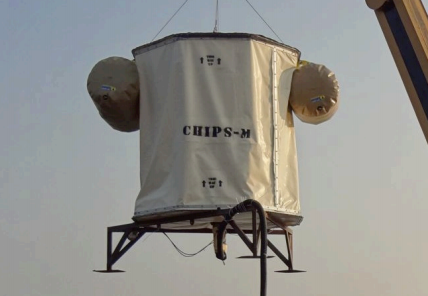
\includegraphics[width=0.6\textwidth]{diagrams/5-chips/chips_m.png}
    \caption[Picture of the \chipsm detector.]
    {Picture of the \chipsm detector just before deployment. The umbilical is visable, attached to
        the bottom endcap of the detector.}
    \label{fig:chips_m}
\end{figure}

\section{The \chipsfive detector} %%%%%%%%%%%%%%%%%%%%%%%%%%%%%%%%%%%%%%%%%%%%%%%%%%%%%%%%%%%%%%%%
\label{sec:chips_detector} %%%%%%%%%%%%%%%%%%%%%%%%%%%%%%%%%%%%%%%%%%%%%%%%%%%%%%%%%%%%%%%%%%%%%%%

- The chips-5 detector is the first of these units, at 25m in diameter and 12m tall.
- This leads to a fiducial volume of ~5kton
- Will be initially deployed into the Wentworth Pit 2W in northen minnesota, which is 7 mrad
off-axis of the numi beam.
- Also deep enough to allow for ~50m of everburden of water to reduce the cosmic background.
- Not at the ideal location (baseline) to measure the mass hierarchy in the Numi beam.
- Can help to constrain delta-cp by measuring electron neutrino appearance.
- Physics capabilities have been studied using GLoBES, should ask Tom for a nice plot and brief
description of how it all works.
- Wentworth 2W is a disused surface iron pit (taconite ore) owned by Cliffs natural resources.
- Has advantages of having the infastrucutre in place for heavy industry, such as power and roads.
- The main Polymet mining building is less than a mile from the deployment site which was used as
a laboratory environment for building detector compoenents on site.
- located at a latitude of 47.58N and longitude of 92.13W. It is 7 mrad off the centralaxis of the
NuMI beam at a baseline of 712 km
- Water is drained from the pit in the spring to ensure it does not overflow during the summer
rainy season.
- Therefore, fluctutationsof +-3m are expected over the course of a year.
- A lighttight liner a polymer membrance is used to seperate the clean detector water from the
external pit water and isolate the detector volume.
- This detector will act as a proff of concept that the R\&D has been a success and the provide
possible improvements for future iterations.
- CHIPS will not initially have a near detector, however the use of NOVA one is possible if
required, but not important for now.
- You would really need a water cherenkov near detector, so it as simiar as possible as the far
detector.
- This allows the same event reco and PID minimising systematic uncertainties in the predicted
background at the far detector.
- Is prefered as it has the same neutrino interaction traget (water) ensuring efficiencies are
similar in both detector.
- However, it should be noted that a water cherenkov detector has never been proven in high
intensity environmenets such as the Numi beam (WTF is t2k then)

INFO: detector module
- Dimensions
- Inner surface area
- PMT diameter
- photocathode coverage in different regions
- No of PMTs
- overburden
- CR muon rate
- In-spill CR occupancy
- CR event dead time
- Veto dimensions
- Veto num PMTs
- veto photocathode coverage
- veto pmt diameter

\begin{figure} % CHIPS SUNRISE DIAGRAM %
    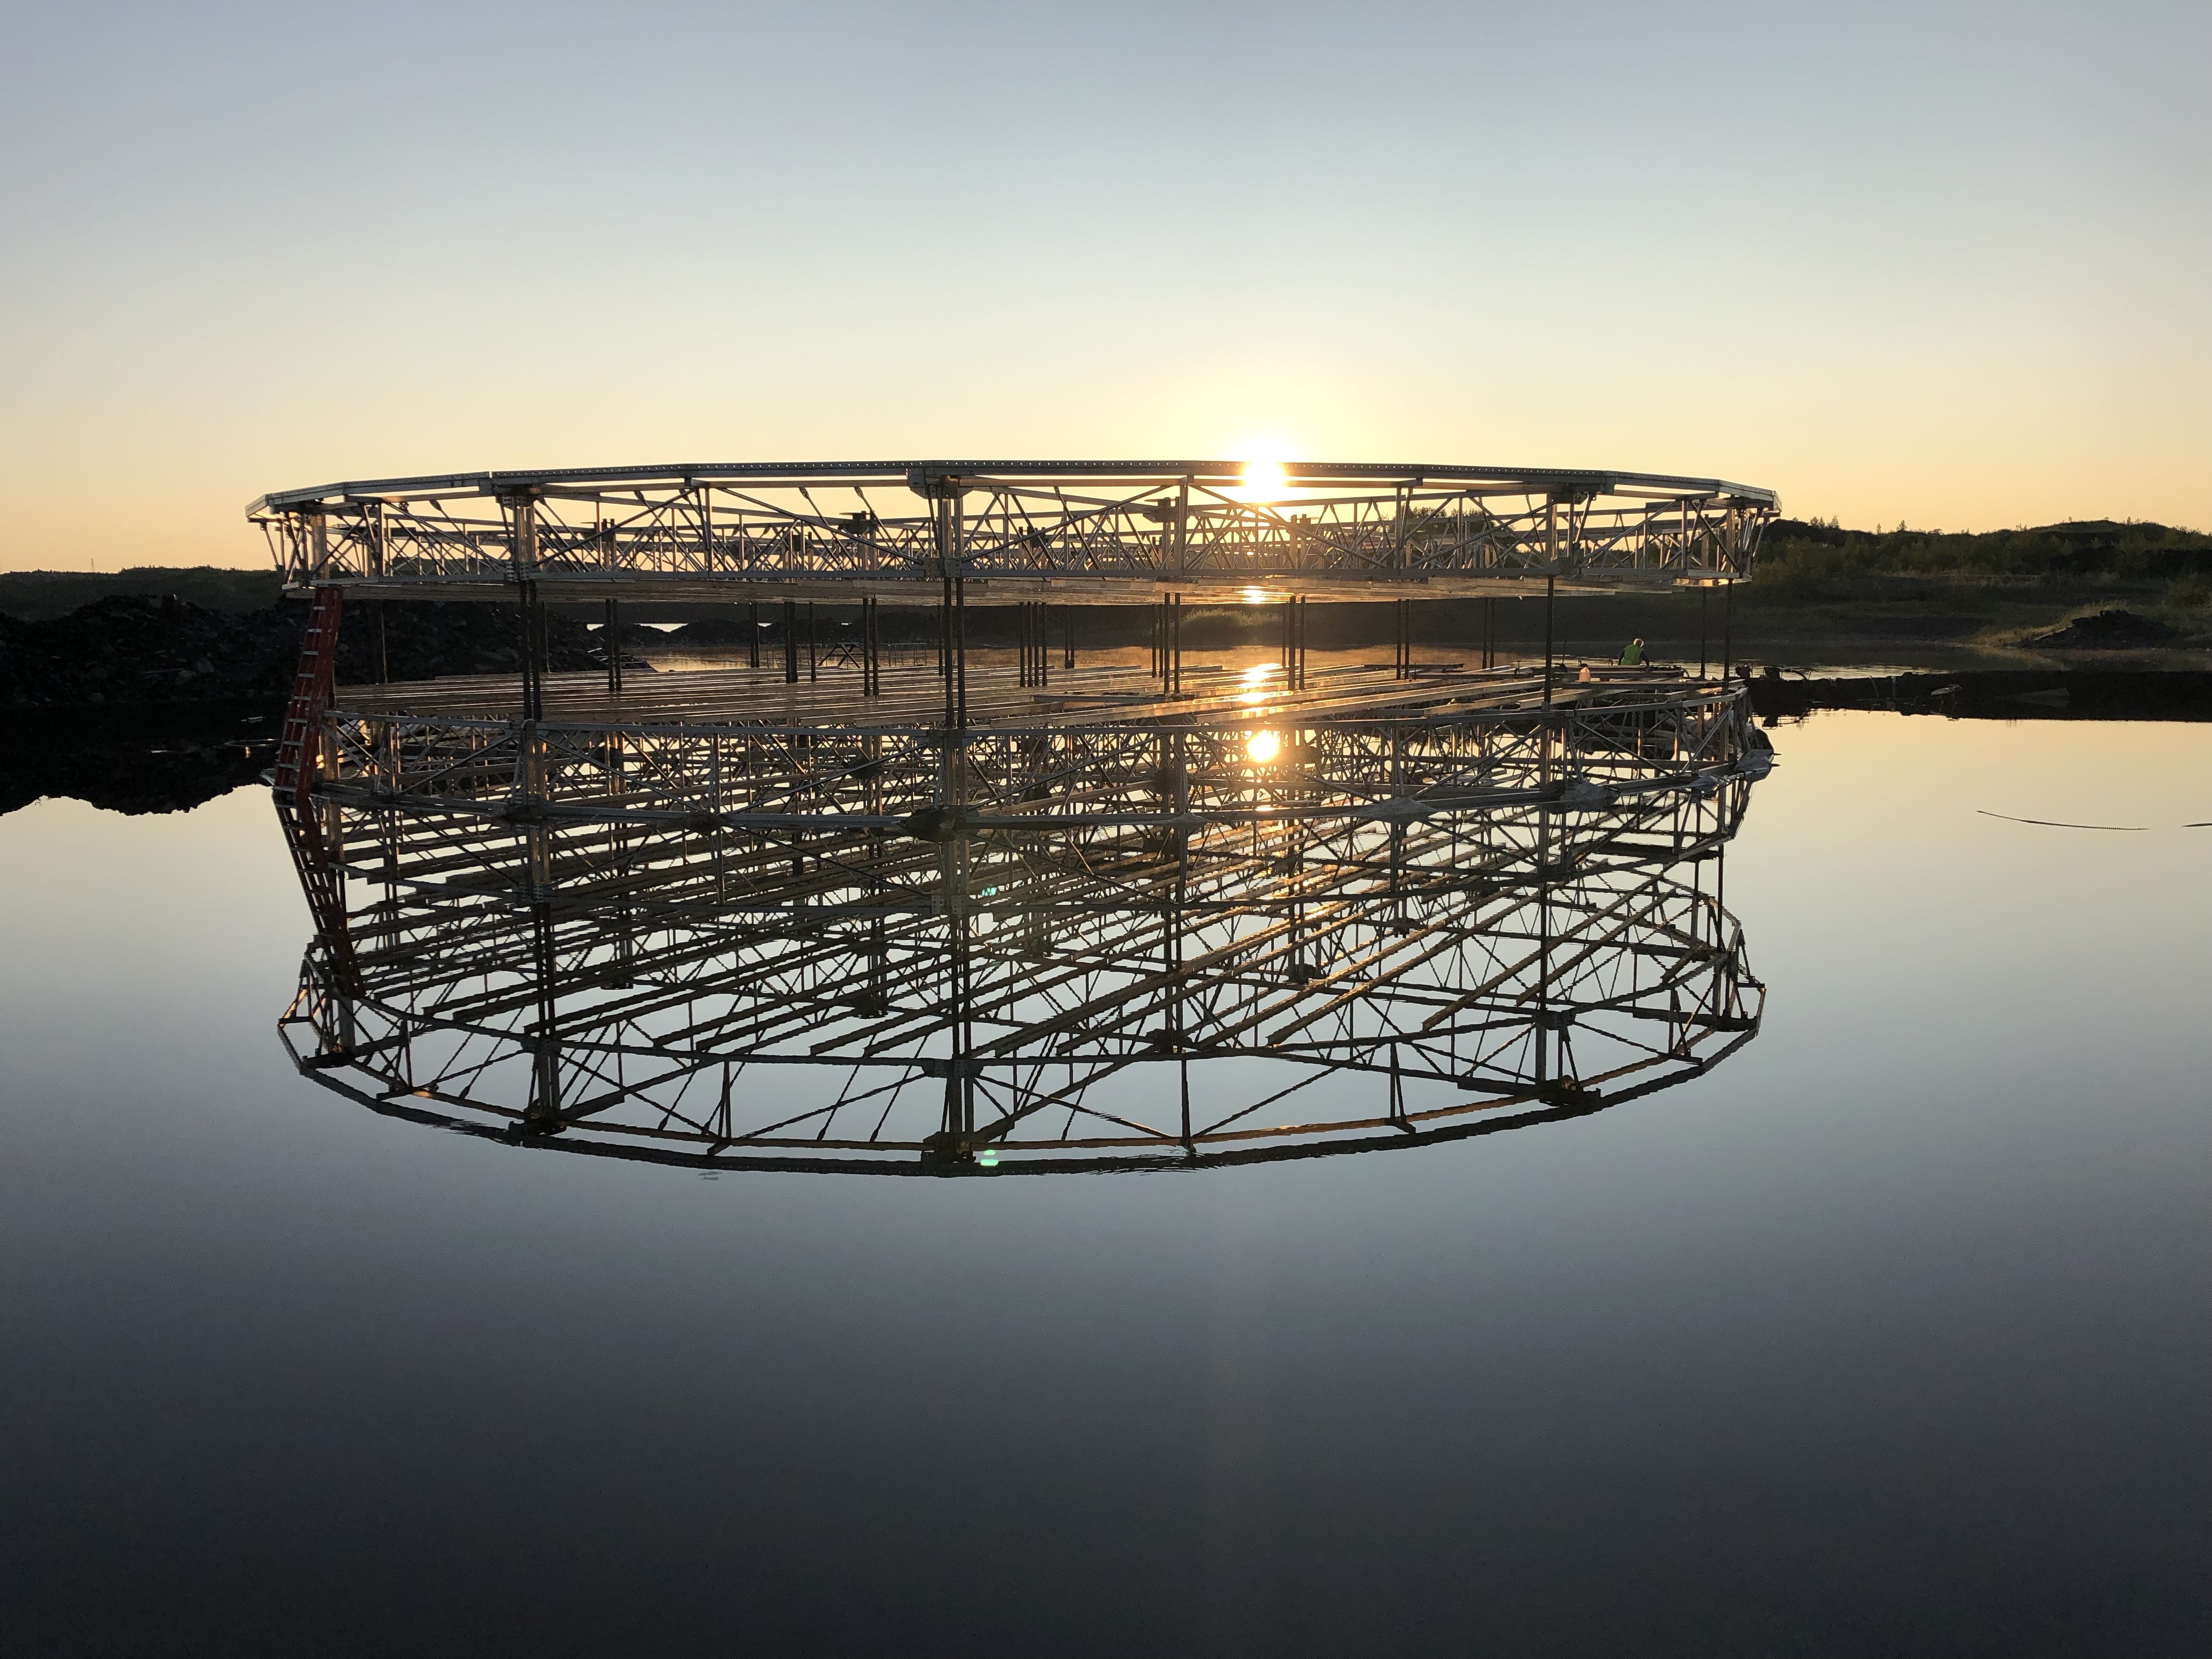
\includegraphics[width=0.6\textwidth]{diagrams/5-chips/sunrise.jpeg}
    \caption[Sunrise over the \chips detector.]
    {Sunrise over the \chips detector structure. The perfectly calm pit water
        produces the mirror effect.}
    \label{fig:sunrise}
\end{figure}

\begin{figure} % CHIPS FROM THE SKY DIAGRAM %
    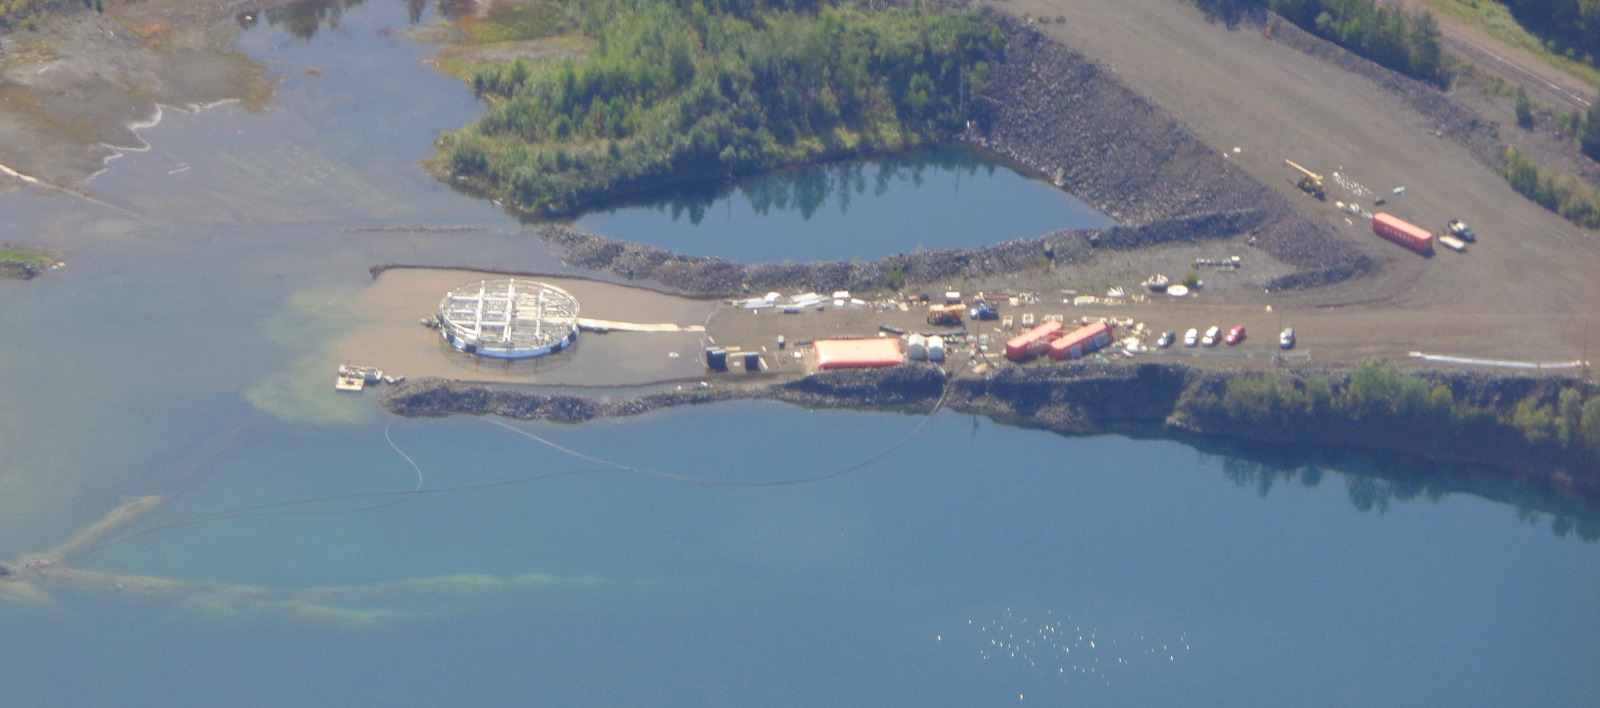
\includegraphics[width=0.6\textwidth]{diagrams/5-chips/from_the_sky.jpg}
    \caption[Picture of the \chips detector from the air.]
    {Picture of the \chips detector taken from an airplane. The Wentworth 2W pit is in the lower
        half of the image, with the half built detector, huts and construction containers
        visable.}
    \label{fig:from_the_sky}
\end{figure}

\begin{figure} % PIT DIAGRAM %
    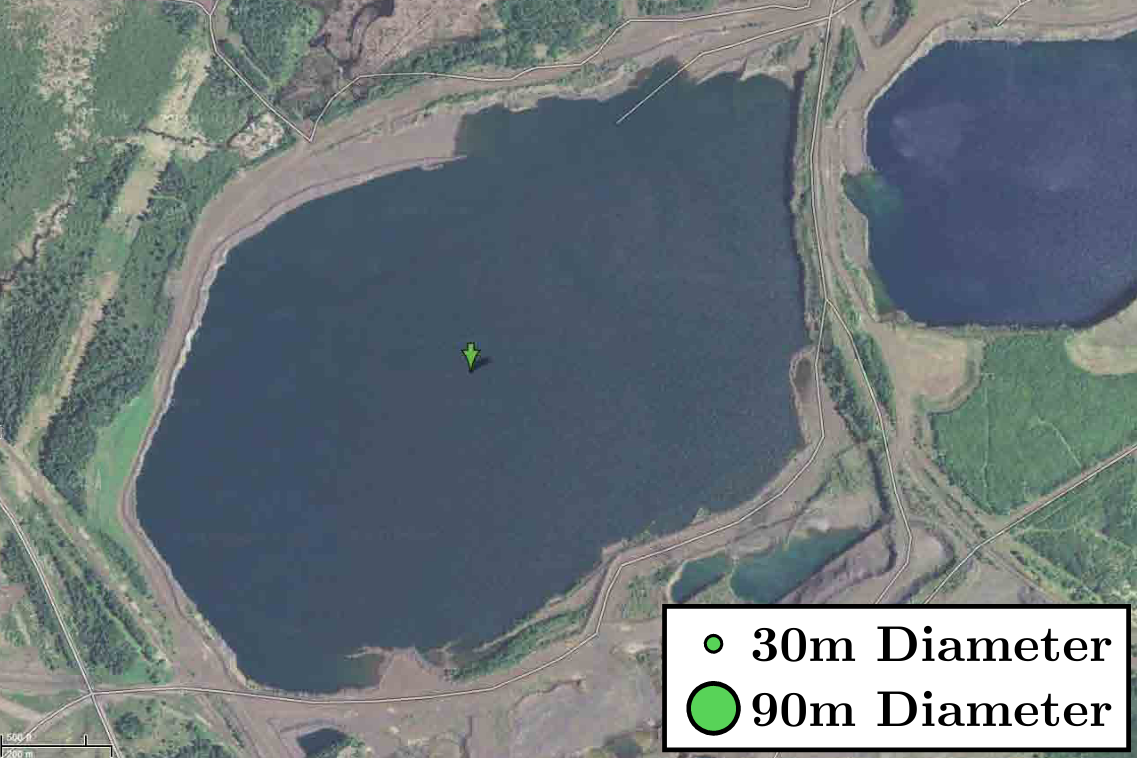
\includegraphics[width=0.6\textwidth]{diagrams/5-chips/location.png}
    \caption[Satellite view of the Wentworth 2W mine pit.]
    {Satellite view of the Wentworth 2W mine pit in northern Minnesota.
        The size markers are shown for scale. Image taken from Ref.\cite{adamson2013}.}
    \label{fig:location}
\end{figure}

\begin{figure} % PIT CONTOUR DIAGRAM %
    \includegraphics[width=0.6\textwidth]{diagrams/5-chips/contour_map.pdf}
    \caption[Topographic map of the Wentworth 2W mine pit.]
    {Topographic map of the Wentworth 2W mine pit. The contours are given in intervals of 5 feet,
        with the central areas of the pit having a depth of 50m. Image taken from
        Ref.\cite{adamson2013}.}
    \label{fig:contour_map}
\end{figure}

\begin{figure} % CHIPS LOCATION IN NUMI DIAGRAM %
    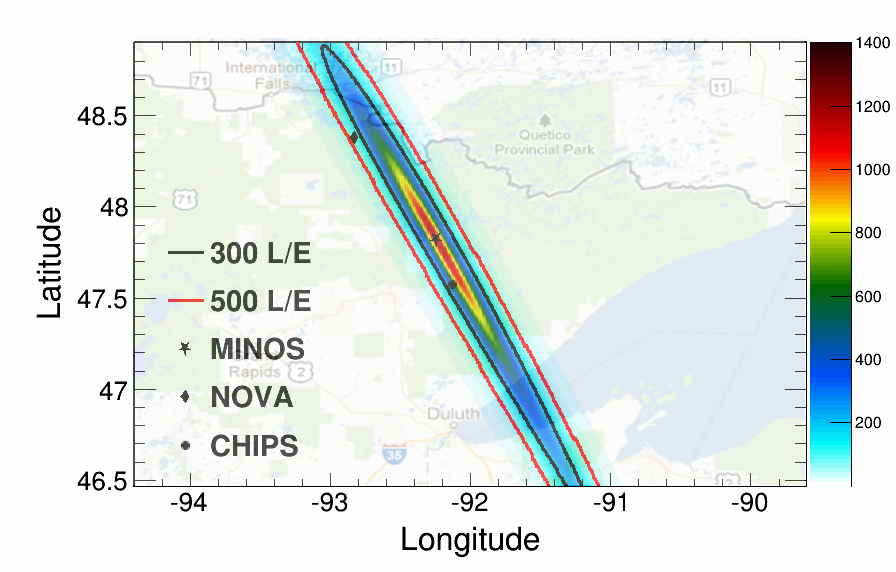
\includegraphics[width=0.6\textwidth]{diagrams/5-chips/numi_map.png}
    \caption[Map of detector locations in the \numi beam.]
    {Map of the \chips, \nova and \minos locations in the \numi beam showing the expected
        neutrino event rates, assuming no oscillations. Lines of constant L/E are shown by the
        contours. Image taken from Ref.\cite{adamson2013}.}
    \label{fig:numi_map}
\end{figure}

\subsection{Structure} %%%%%%%%%%%%%%%%%%%%%%%%%%%%%%%%%%%%%%%%%%%%%%%%%%%%%%%%%%%%%%%%%%%%%%%%%%%
\label{sec:chips_detector_structure} %%%%%%%%%%%%%%%%%%%%%%%%%%%%%%%%%%%%%%%%%%%%%%%%%%%%%%%%%%%%%

\begin{figure} % CHIPS RENDER 1 DIAGRAM %
    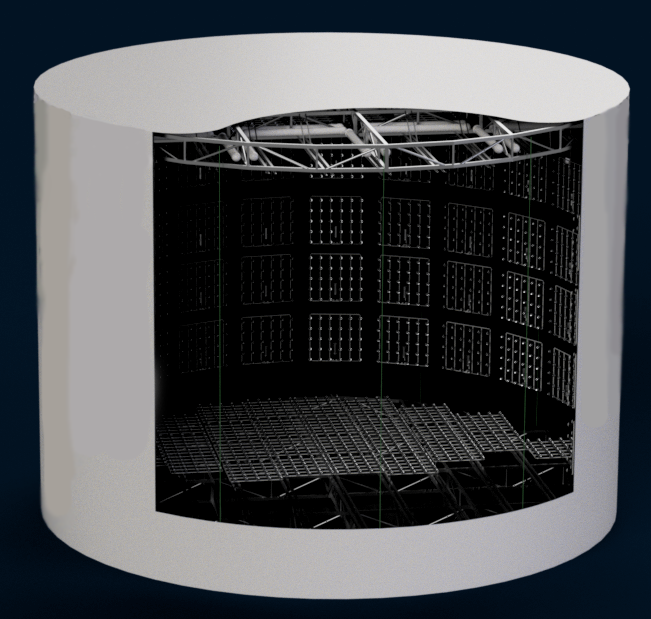
\includegraphics[width=0.6\textwidth]{diagrams/5-chips/chips_render_1.png}
    \caption[Graphical rendering of the \chipsfive detector with liner cutaway.]
    {Graphical rendering of the \chipsfive detector with a section of the liner cutaway.
        The bottom endcap and wall planes are visable,
        as well as the top endcap structure and floatation.}
    \label{fig:chips_render_1}
\end{figure}

\begin{figure} % CHIPS RENDER 2 DIAGRAM %
    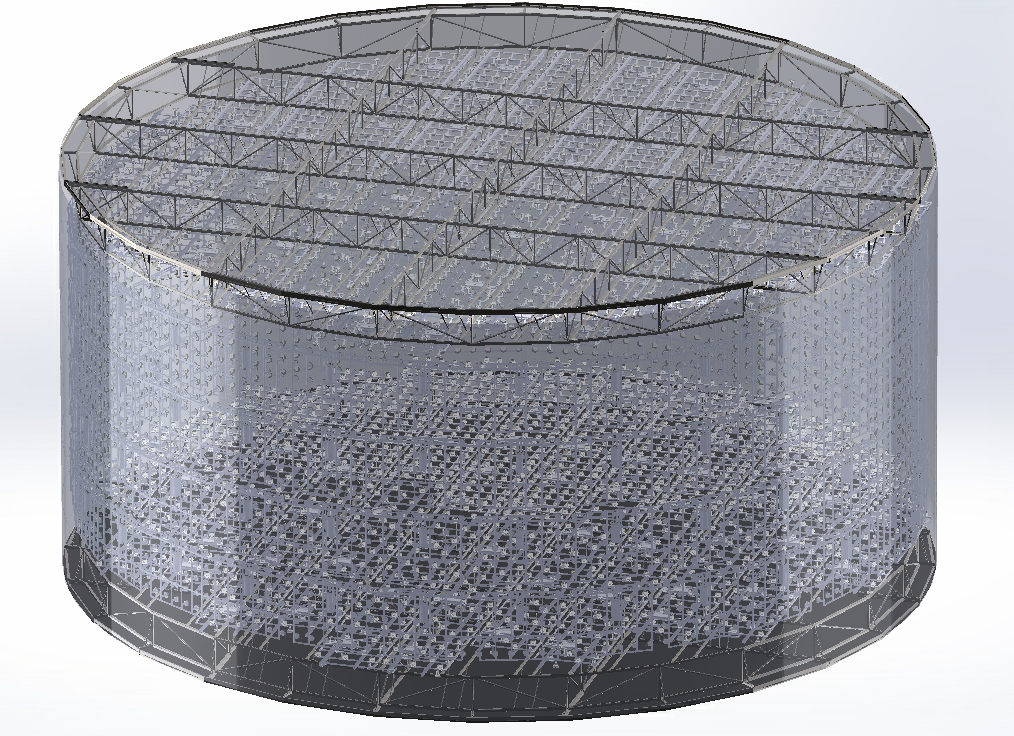
\includegraphics[width=0.6\textwidth]{diagrams/5-chips/chips_render_2.png}
    \caption[Graphical rendering of the \chipsfive detector structure.]
    {Graphical rendering of the \chipsfive detector structure.}
    \label{fig:chips_render_2}
\end{figure}

\subsection{Instrumentation} %%%%%%%%%%%%%%%%%%%%%%%%%%%%%%%%%%%%%%%%%%%%%%%%%%%%%%%%%%%%%%%%%%%%%
\label{sec:chips_detector_instrumentation} %%%%%%%%%%%%%%%%%%%%%%%%%%%%%%%%%%%%%%%%%%%%%%%%%%%%%%%

km3net 2.0 ref in \cite{adrian2016}
Icecube DOM paper \cite{hanson2006}


DIAGRAM: POM diagram
REF: Icecube DOM paper
REF: Km3net optical module paper
REF: Nemo-3 PMT paper
- CHIPS uses high quantum efficiency PMTs from Hamamatsu
REF: Get hamamatsu PMT reference
- We will talk in detail about DAQ in the following chapter
- For calibration "flashers" are built into the detector to allow for known location light
generation to calibrate final PMT positions and time resolutuions.

\begin{figure} % PMT ASSEMBLY DIAGRAM %
    \centering
    \subcaptionbox{pmt disassembled\label{fig:pmt_disassembled}}{%
        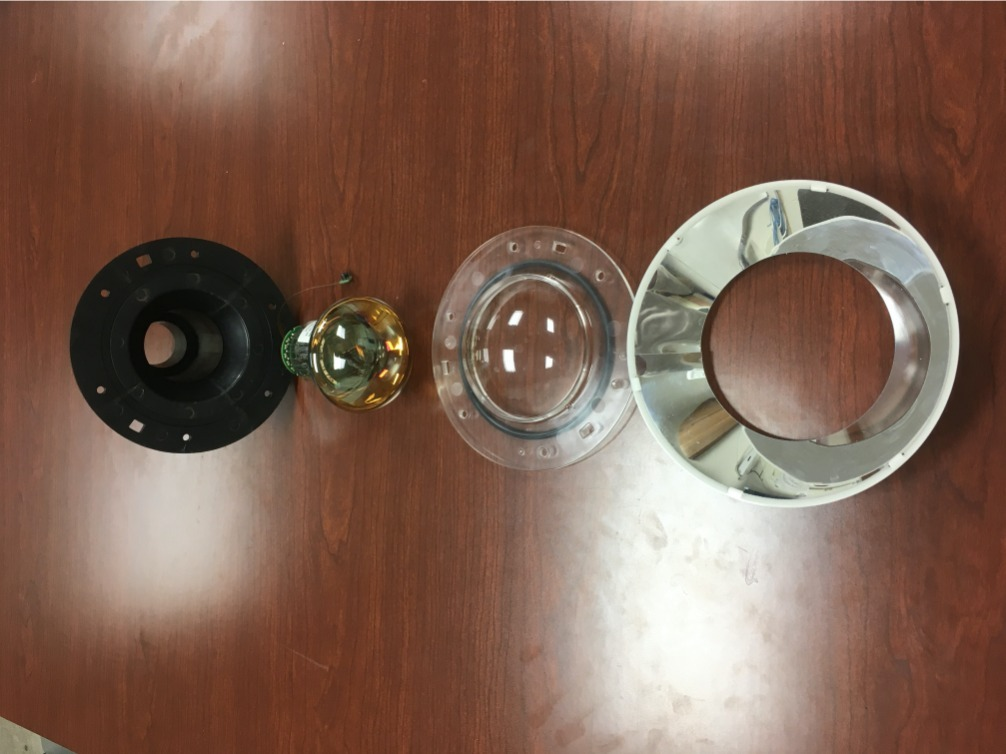
\includegraphics[height=5cm]{diagrams/5-chips/pmt_disassembled.jpg}%
    }
    \quad
    \subcaptionbox{pmt assembled\label{fig:pmt_assembled}}{%
        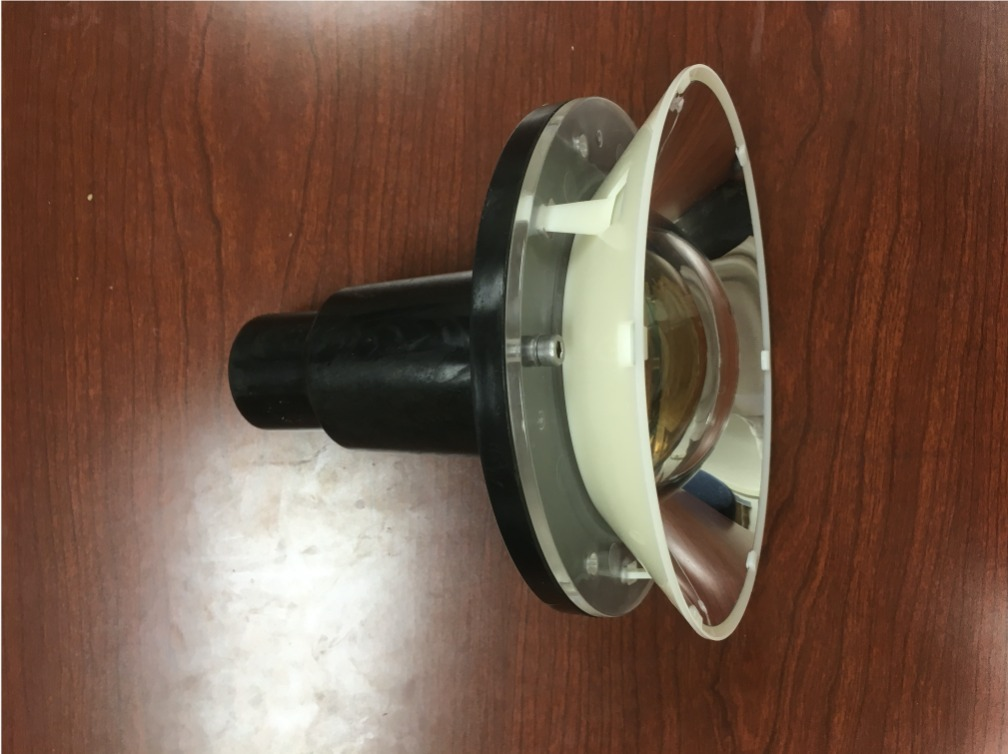
\includegraphics[height=5cm]{diagrams/5-chips/pmt_assembled.jpg}%
    }
    \caption[The caption]
    {The caption}
\end{figure}

\begin{figure} % NIKHEF PLANE DIAGRAM %
    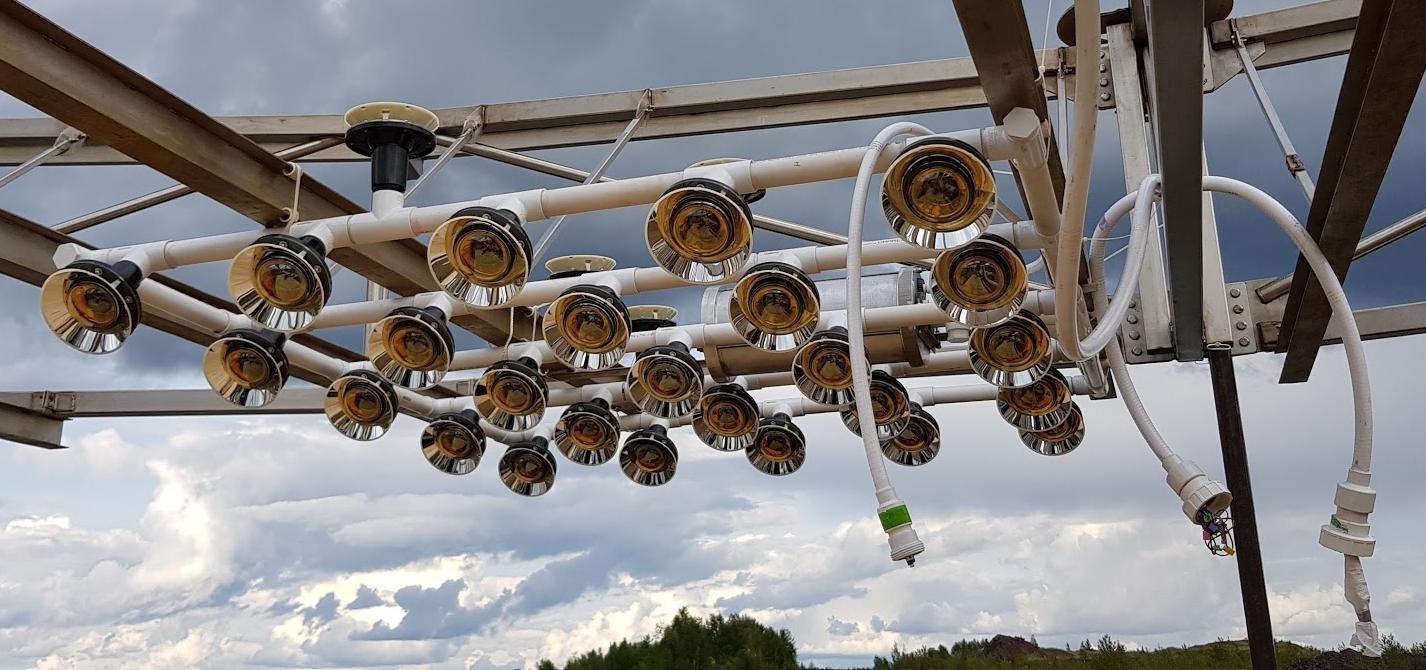
\includegraphics[width=0.8\textwidth]{diagrams/5-chips/single_plane.jpg}
    \caption[single plane short]
    {single plane long}
    \label{fig:single_plane}
\end{figure}

\subsection{Water clarity} %%%%%%%%%%%%%%%%%%%%%%%%%%%%%%%%%%%%%%%%%%%%%%%%%%%%%%%%%%%%%%%%%%%%%%%
\label{sec:chips_detector_water} %%%%%%%%%%%%%%%%%%%%%%%%%%%%%%%%%%%%%%%%%%%%%%%%%%%%%%%%%%%%%%%%%

- Though remarkably clear the Wentworth pit water is not clean enough for the detector volume
where we require ~30m attenuation length.
- CHIPS attenuation length paper~\cite{amat2017}

\subsection{Deployment} %%%%%%%%%%%%%%%%%%%%%%%%%%%%%%%%%%%%%%%%%%%%%%%%%%%%%%%%%%%%%%%%%%%%%%%%%%
\label{sec:chips_detector_deployment} %%%%%%%%%%%%%%%%%%%%%%%%%%%%%%%%%%%%%%%%%%%%%%%%%%%%%%%%%%%%

DIAGRAM: Floating dock diagram
DIAGRAM: Deployment diagram
- How it can grow if needed

\subsection{Current status} %%%%%%%%%%%%%%%%%%%%%%%%%%%%%%%%%%%%%%%%%%%%%%%%%%%%%%%%%%%%%%%%%%%%%%
\label{sec:chips_detector_status} %%%%%%%%%%%%%%%%%%%%%%%%%%%%%%%%%%%%%%%%%%%%%%%%%%%%%%%%%%%%%%%%

\section{Monte Carlo event generation and simulation} %%%%%%%%%%%%%%%%%%%%%%%%%%%%%%%%%%%%%%%%%%%%
\label{sec:chips_monte_carlo} %%%%%%%%%%%%%%%%%%%%%%%%%%%%%%%%%%%%%%%%%%%%%%%%%%%%%%%%%%%%%%%%%%%%

\subsection{Beam event generation} %%%%%%%%%%%%%%%%%%%%%%%%%%%%%%%%%%%%%%%%%%%%%%%%%%%%%%%%%%%%%%%
\label{sec:chips_monte_carlo_beam} %%%%%%%%%%%%%%%%%%%%%%%%%%%%%%%%%%%%%%%%%%%%%%%%%%%%%%%%%%%%%%%

Cosmic event rate in \cite{son2013}

- We take full advantage of the MINOS, NOVA extensive simulations of the Numi beam for use in
CHIPS.
- The tau neutrino component is negligible and not predicted by the simulation
INFO: expected number of events per year etc...
DIAGRAM: CHIPS expected event rate plot with and without oscillations

\subsection{Cosmic event generation} %%%%%%%%%%%%%%%%%%%%%%%%%%%%%%%%%%%%%%%%%%%%%%%%%%%%%%%%%%%%%
\label{sec:chips_monte_carlo_cosmic} %%%%%%%%%%%%%%%%%%%%%%%%%%%%%%%%%%%%%%%%%%%%%%%%%%%%%%%%%%%%%

DIAGRAM: expected cosmic rate at different height plot
DIAGRAM: Cosmic rate given the water overburden diagram

\begin{figure} % COSMICS AROUND DETECTOR DIAGRAM %
    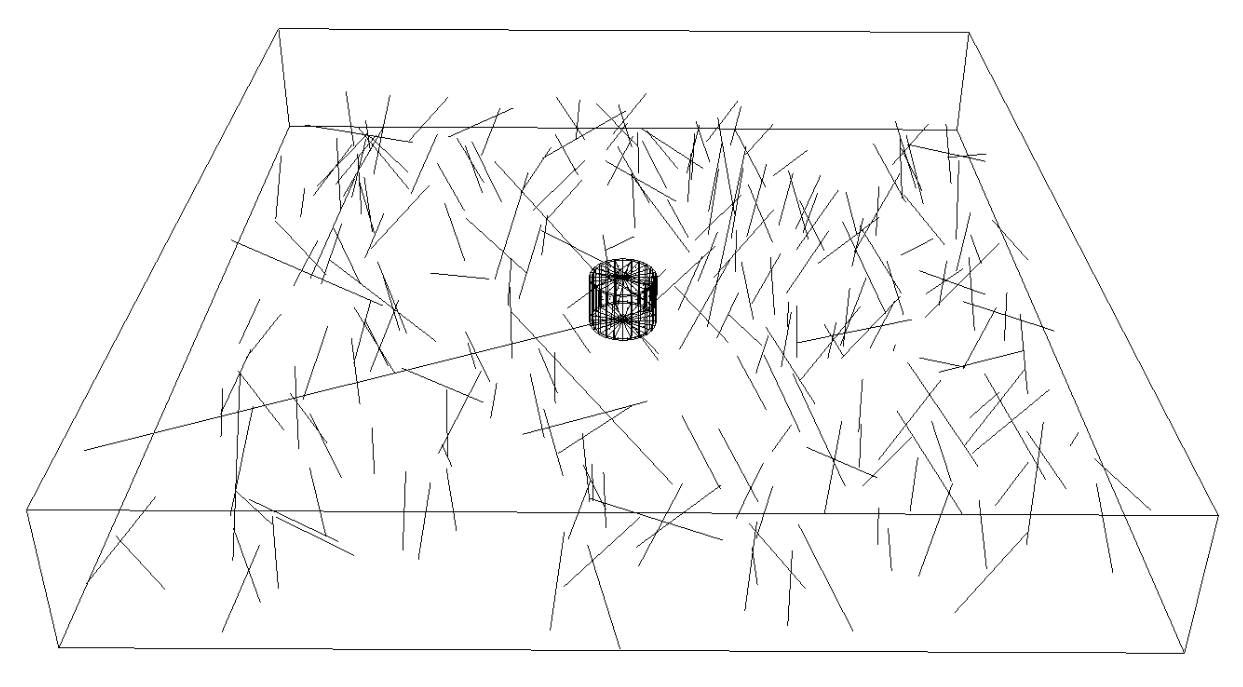
\includegraphics[width=0.8\textwidth]{diagrams/5-chips/cosmics.png}
    \caption[cosmics short]
    {cosmics long}
    \label{fig:cosmics}
\end{figure}

\subsection{Detector simulation} %%%%%%%%%%%%%%%%%%%%%%%%%%%%%%%%%%%%%%%%%%%%%%%%%%%%%%%%%%%%%%%%%
\label{sec:chips_monte_carlo_sim} %%%%%%%%%%%%%%%%%%%%%%%%%%%%%%%%%%%%%%%%%%%%%%%%%%%%%%%%%%%%%%%%

\begin{figure} % SIMULATED EVENT DISPLAY DIAGRAM %
    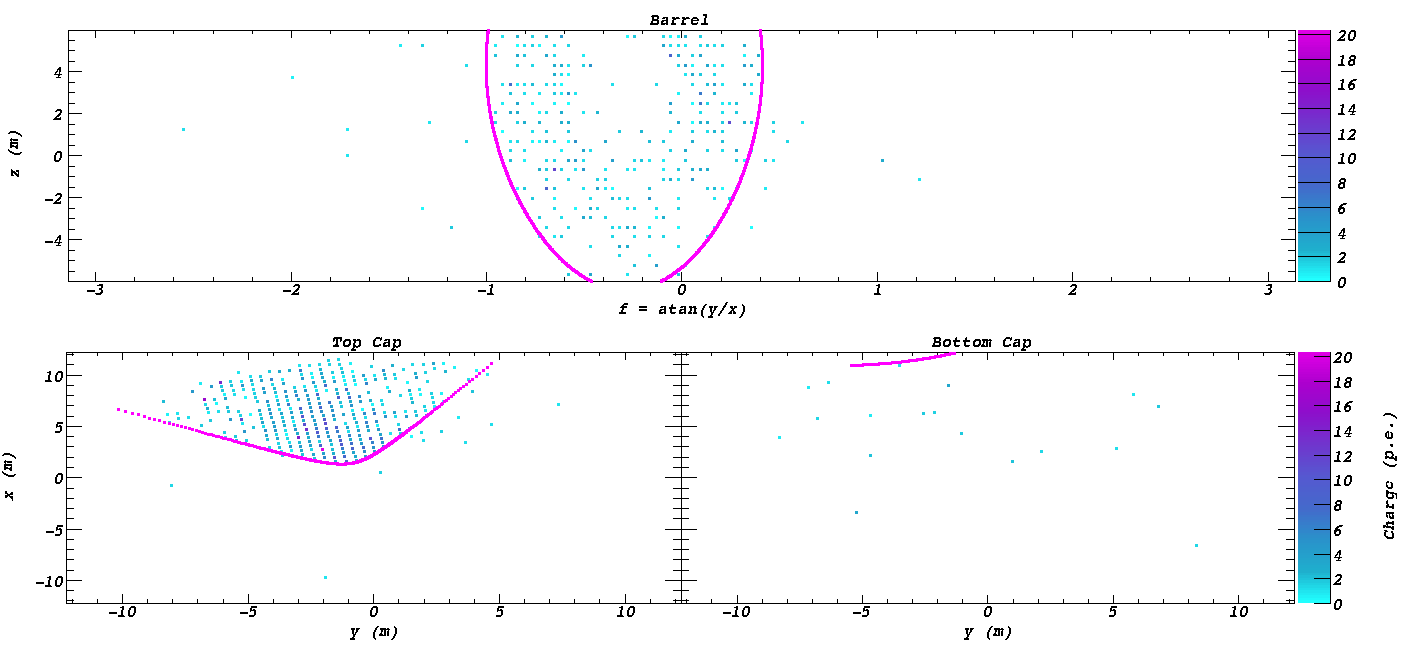
\includegraphics[width=\textwidth]{diagrams/5-chips/sim_event.png}
    \caption[sim event short]
    {$\nu_{\mu}$ CC quasi-elastic event with a single muon final state particle of energy
        1770.24 MeV}
    \label{fig:sim_event}
\end{figure}
    \chapter{Data acquisition for CHIPS} %%%%%%%%%%%%%%%%%%%%%%%%%%%%%%%%%%%%%%%%%%%%%%%%%%%%%%%%%%%%%
\label{chap:daq} %%%%%%%%%%%%%%%%%%%%%%%%%%%%%%%%%%%%%%%%%%%%%%%%%%%%%%%%%%%%%%%%%%%%%%%%%%%%%%%%%

\begin{comment} % PLAN %%%%%%%%%%%%%%%%%%%%%%%%%%%%%%%%%%%%%%%%%%%%%%%%%%%%%%%%%%%%%%%%%%%%%%%%%%%

- What makes this implementation special
- Limited resource, but brilliant capabilities
- Use existing software when possible

HARDWARE
- The White Rabbit timing system
- Km3NET hardware
- Madison hardware (novel)
- Combined systems

SOFTWARE
- The beam spill
- Hit acquisition and handling
- Detector and data quality monitoring
\end{comment}

TODO: Add labels to picture diagrams in a tasteful way

\section{Hardware} %%%%%%%%%%%%%%%%%%%%%%%%%%%%%%%%%%%%%%%%%%%%%%%%%%%%%%%%%%%%%%%%%%%%%%%%%%%%%%%
\label{sec:daq_hard} %%%%%%%%%%%%%%%%%%%%%%%%%%%%%%%%%%%%%%%%%%%%%%%%%%%%%%%%%%%%%%%%%%%%%%%%%%%%%

\subsection{The White Rabbit timing system} %%%%%%%%%%%%%%%%%%%%%%%%%%%%%%%%%%%%%%%%%%%%%%%%%%%%%%
\label{sec:daq_hard_timing} %%%%%%%%%%%%%%%%%%%%%%%%%%%%%%%%%%%%%%%%%%%%%%%%%%%%%%%%%%%%%%%%%%%%%%

REF: White-rabbit papers

\begin{figure} % WHITE-RABBIT SWITCH DIAGRAM %
    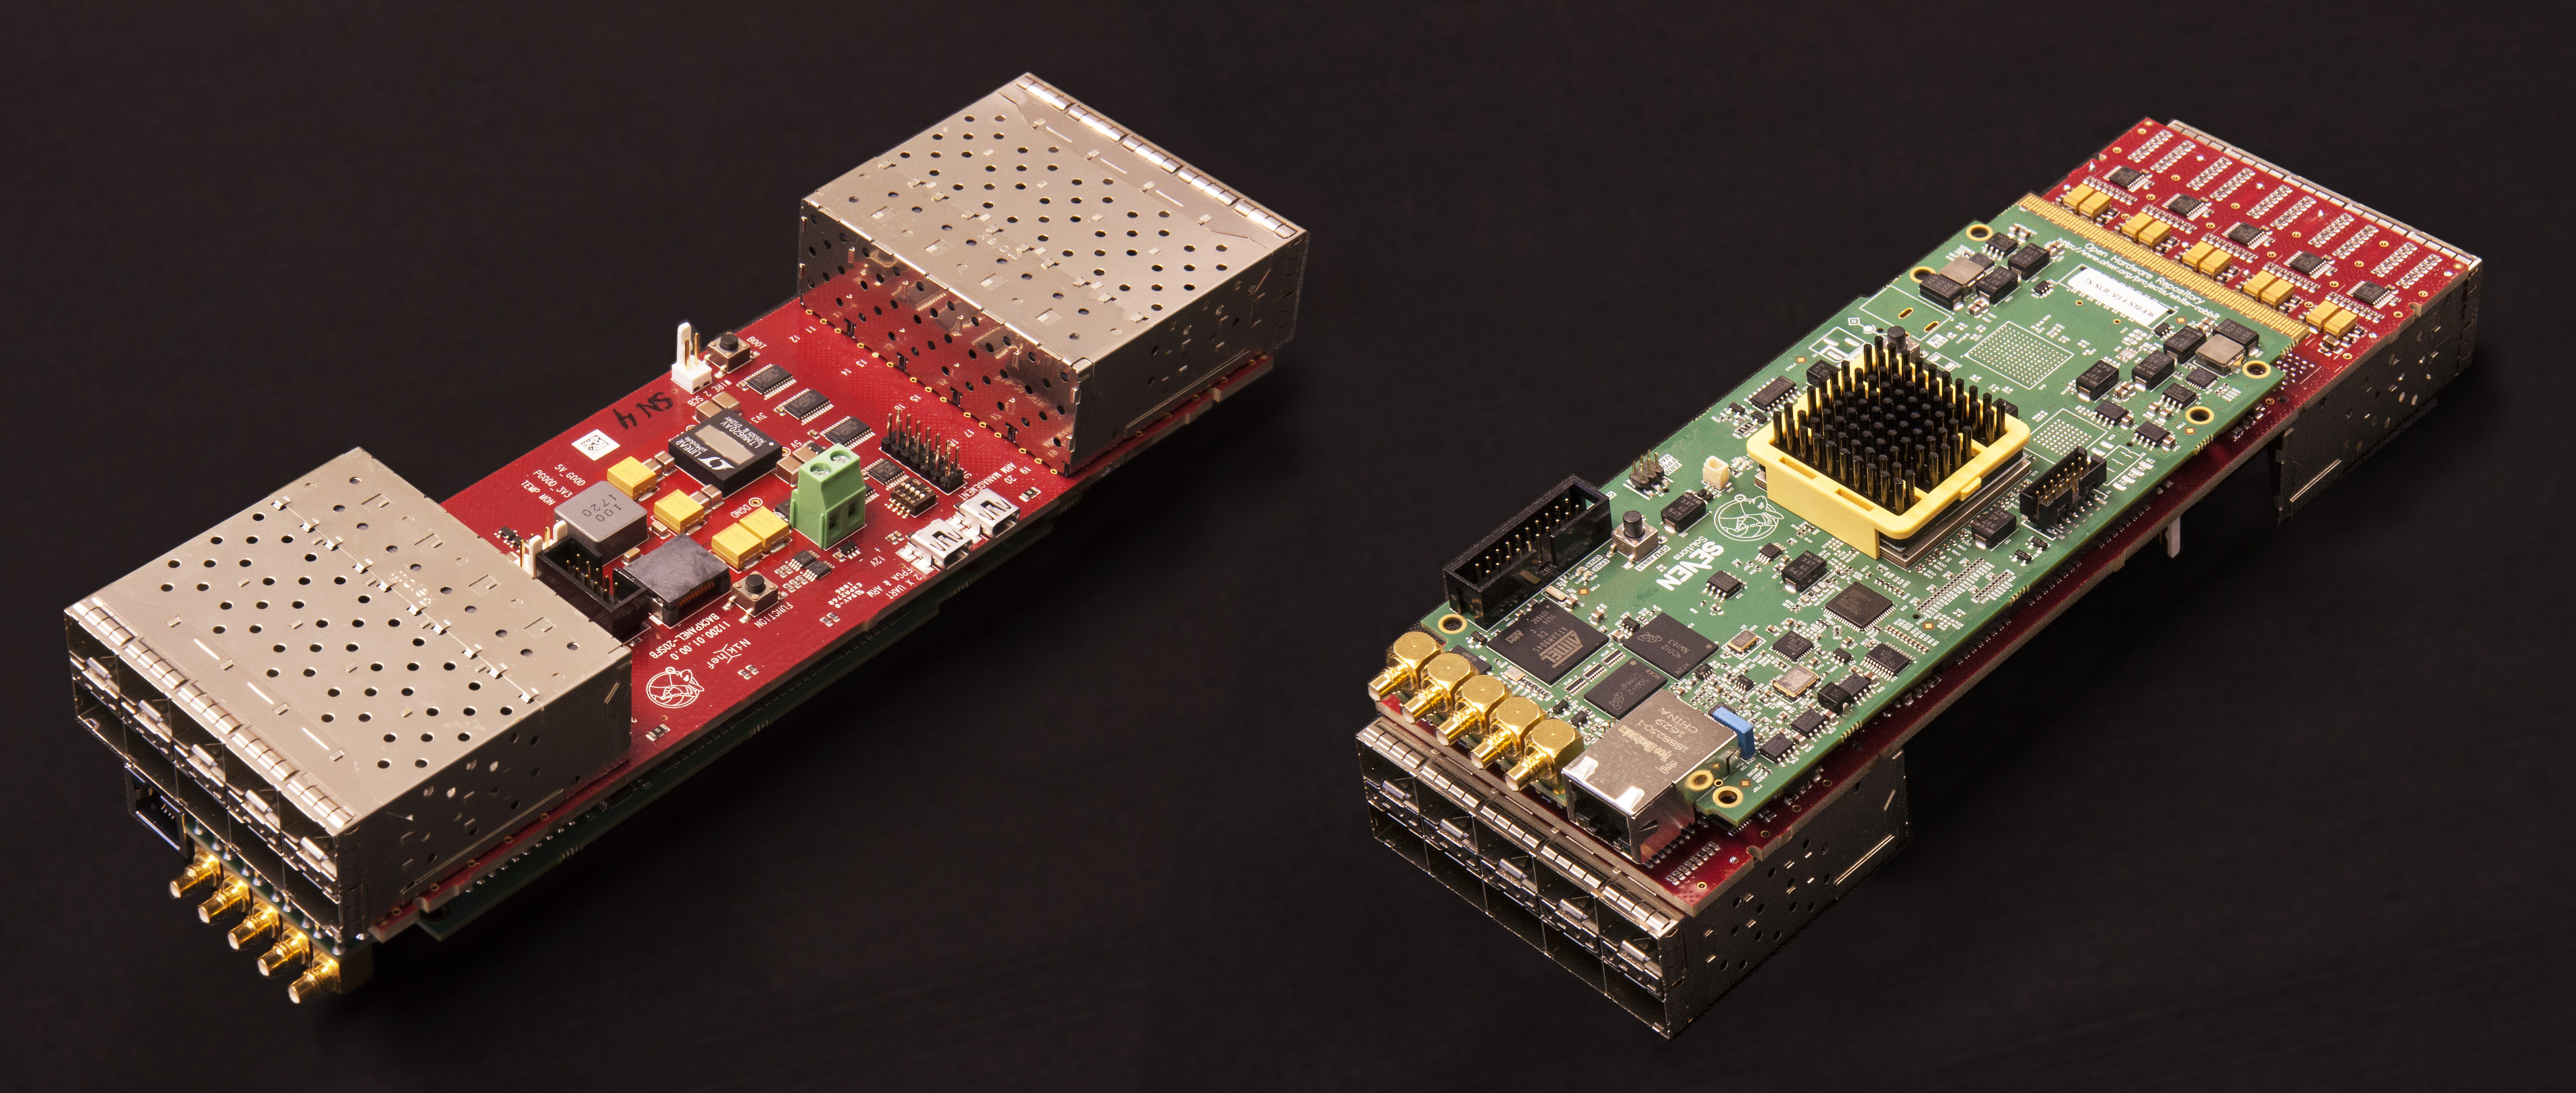
\includegraphics[width=\textwidth]{diagrams/6-daq/wr_switch.jpg}
    \caption[wr switch short]
    {wr switch long}
    \label{fig:wr_switch}
\end{figure}

\begin{figure} % WHITE-RABBIT SYNC DIAGRAM %
    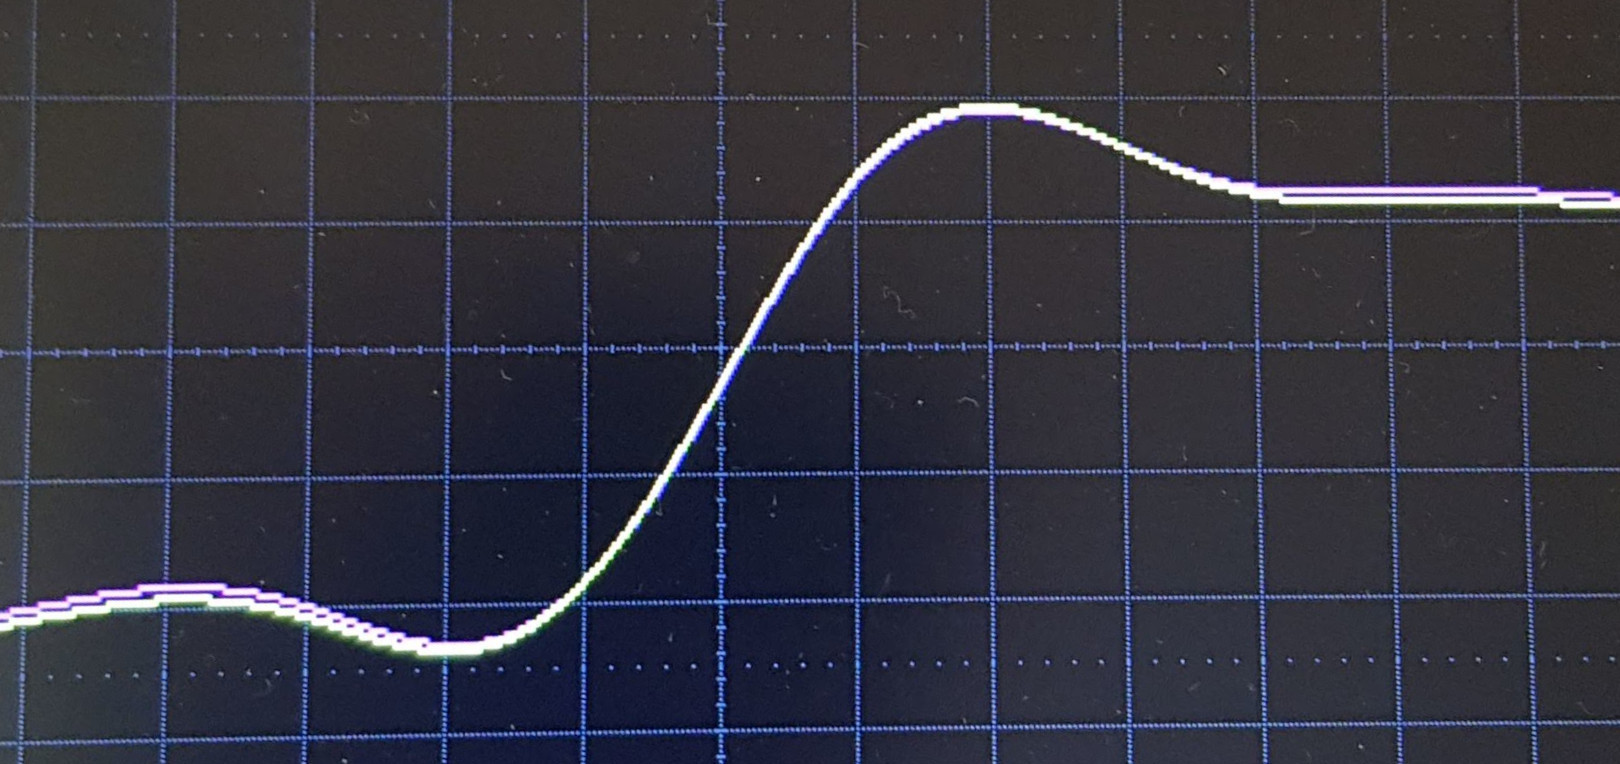
\includegraphics[width=0.8\textwidth]{diagrams/6-daq/sync.jpg}
    \caption[sync short]
    {sync long}
    \label{fig:sync}
\end{figure}

\subsection{Km3NET hardware} %%%%%%%%%%%%%%%%%%%%%%%%%%%%%%%%%%%%%%%%%%%%%%%%%%%%%%%%%%%%%%%%%%%%%
\label{sec:daq_hard_km3net} %%%%%%%%%%%%%%%%%%%%%%%%%%%%%%%%%%%%%%%%%%%%%%%%%%%%%%%%%%%%%%%%%%%%%%

DIAGRAM: Nikhef hardware diagram
REF: PMT time resolution papers
REF: km3net DAQ papers

\begin{figure} % NIKHEF PMT AND CLB DIAGRAM %
    \centering
    \subcaptionbox{nikhef pmt\label{fig:nikhef_pmt}}{%
        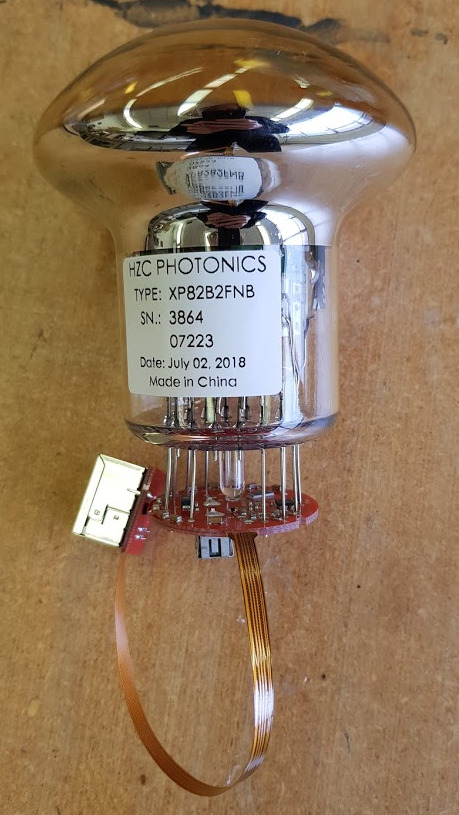
\includegraphics[height=8cm]{diagrams/6-daq/nikhef_pmt.jpg}%
    }
    \quad
    \subcaptionbox{clb\label{fig:clb}}{%
        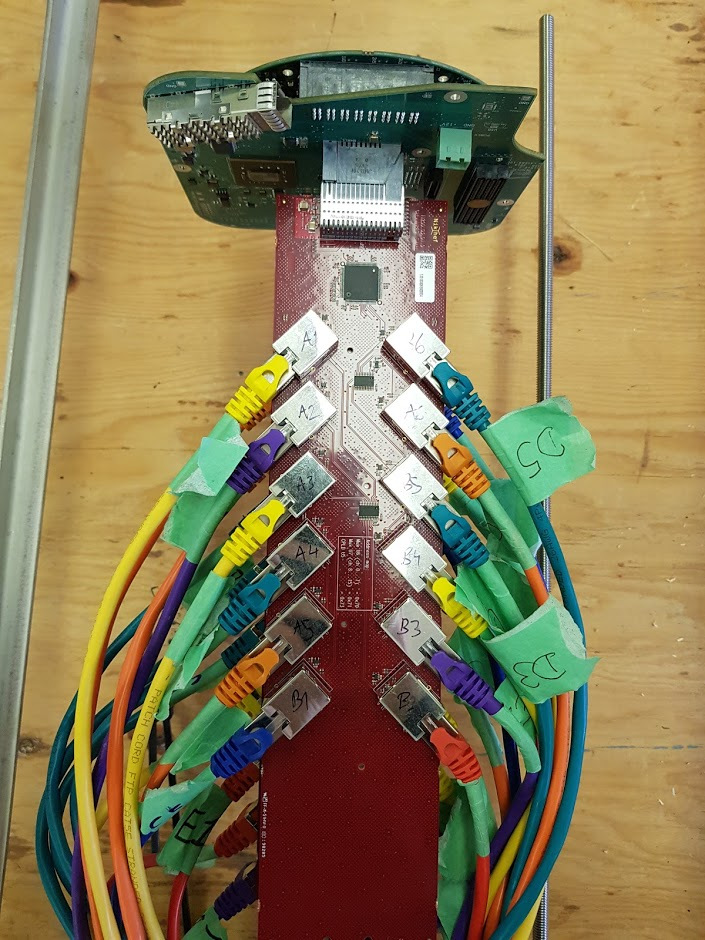
\includegraphics[height=8cm]{diagrams/6-daq/clb.jpg}%
    }
    \caption[The caption]
    {The caption}
\end{figure}

\begin{figure} % CLB ROCKETS DIAGRAM %
    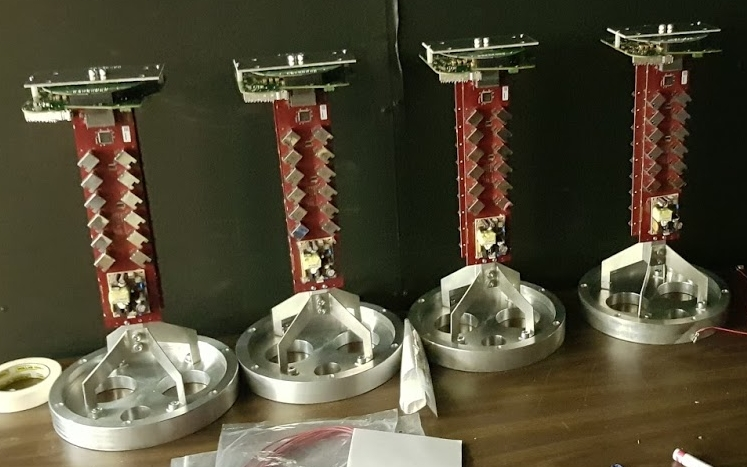
\includegraphics[width=0.6\textwidth]{diagrams/6-daq/rockets.jpg}
    \caption[rockets short]
    {rockets long}
    \label{fig:rockets}
\end{figure}

\subsection{Madison hardware} %%%%%%%%%%%%%%%%%%%%%%%%%%%%%%%%%%%%%%%%%%%%%%%%%%%%%%%%%%%%%%%%%%%%
\label{sec:daq_hard_madison} %%%%%%%%%%%%%%%%%%%%%%%%%%%%%%%%%%%%%%%%%%%%%%%%%%%%%%%%%%%%%%%%%%%%%

DIAGRAM: Madison hardware diagram

\begin{figure} % WR-LEN DIAGRAM %
    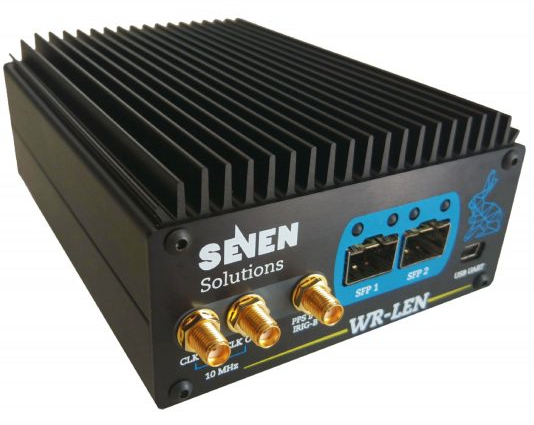
\includegraphics[width=0.8\textwidth]{diagrams/6-daq/wr_len.jpg}
    \caption[wr len short]
    {wr len long}
    \label{fig:wr_len}
\end{figure}

\begin{figure} % TOT DIAGRAM DIAGRAM %
    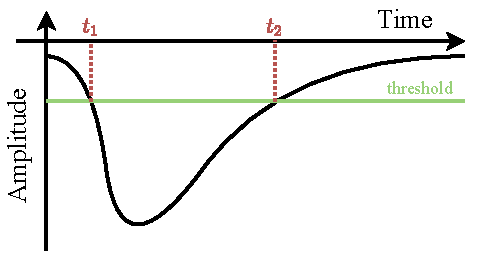
\includegraphics[width=0.6\textwidth]{diagrams/6-daq/tot.pdf}
    \caption[tot short]
    {tot long}
    \label{fig:tot}
\end{figure}

\begin{figure} % BEAGLEBONE AND DANOUT DIAGRAM %
    \centering
    \subcaptionbox{beaglebone\label{fig:beaglebone}}{%
        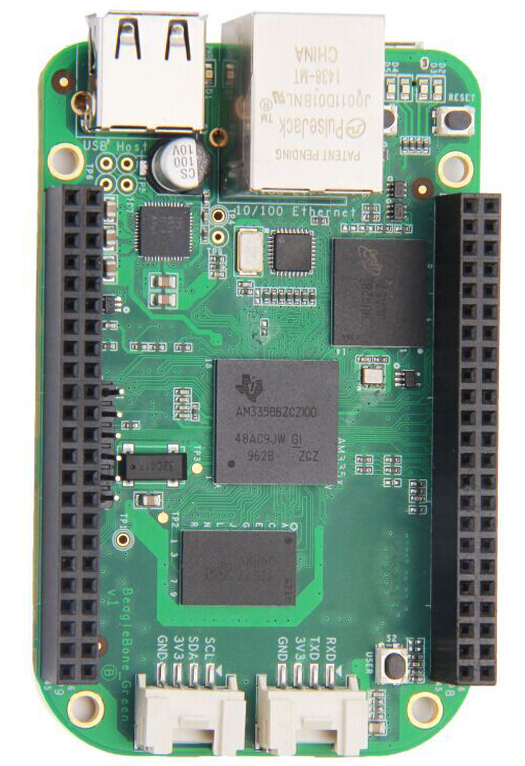
\includegraphics[height=6cm]{diagrams/6-daq/beaglebone.jpg}%
    }
    \quad
    \subcaptionbox{danout\label{fig:danout}}{%
        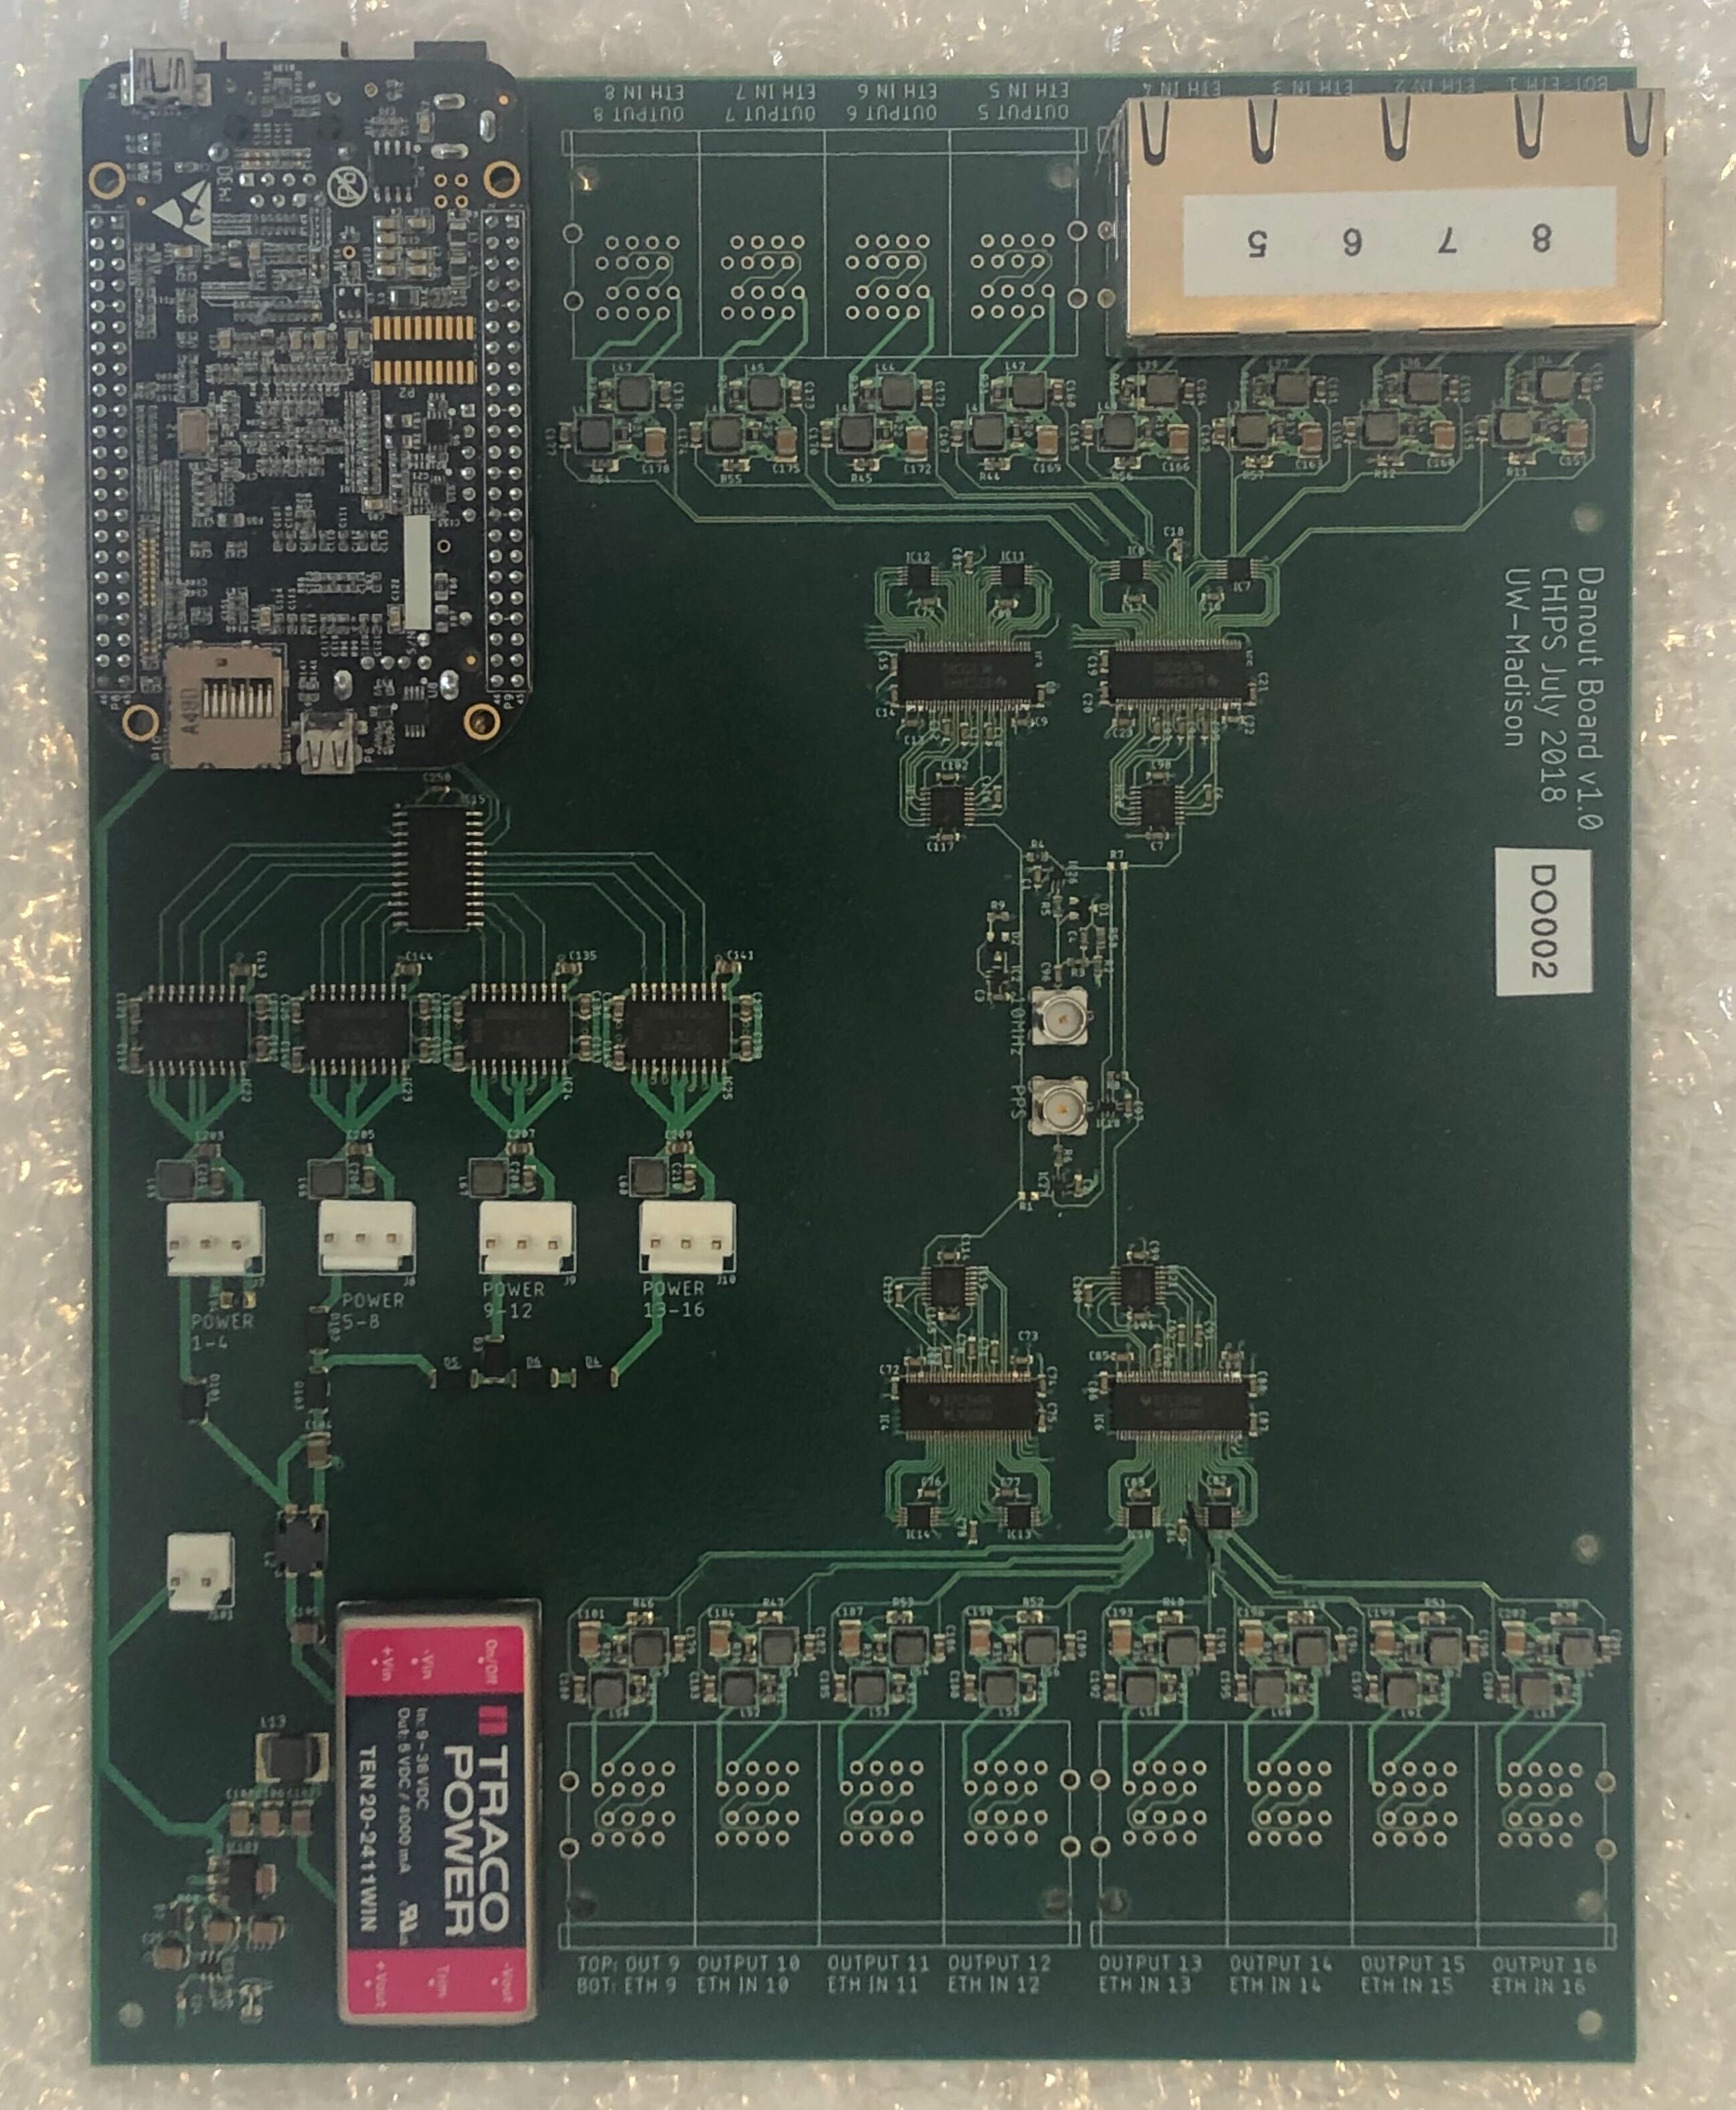
\includegraphics[angle=90, height=6cm]{diagrams/6-daq/danout.jpg}%
    }
    \caption[The caption]
    {The caption}
\end{figure}

\begin{figure} % BADGER BOARD DIAGRAM %
    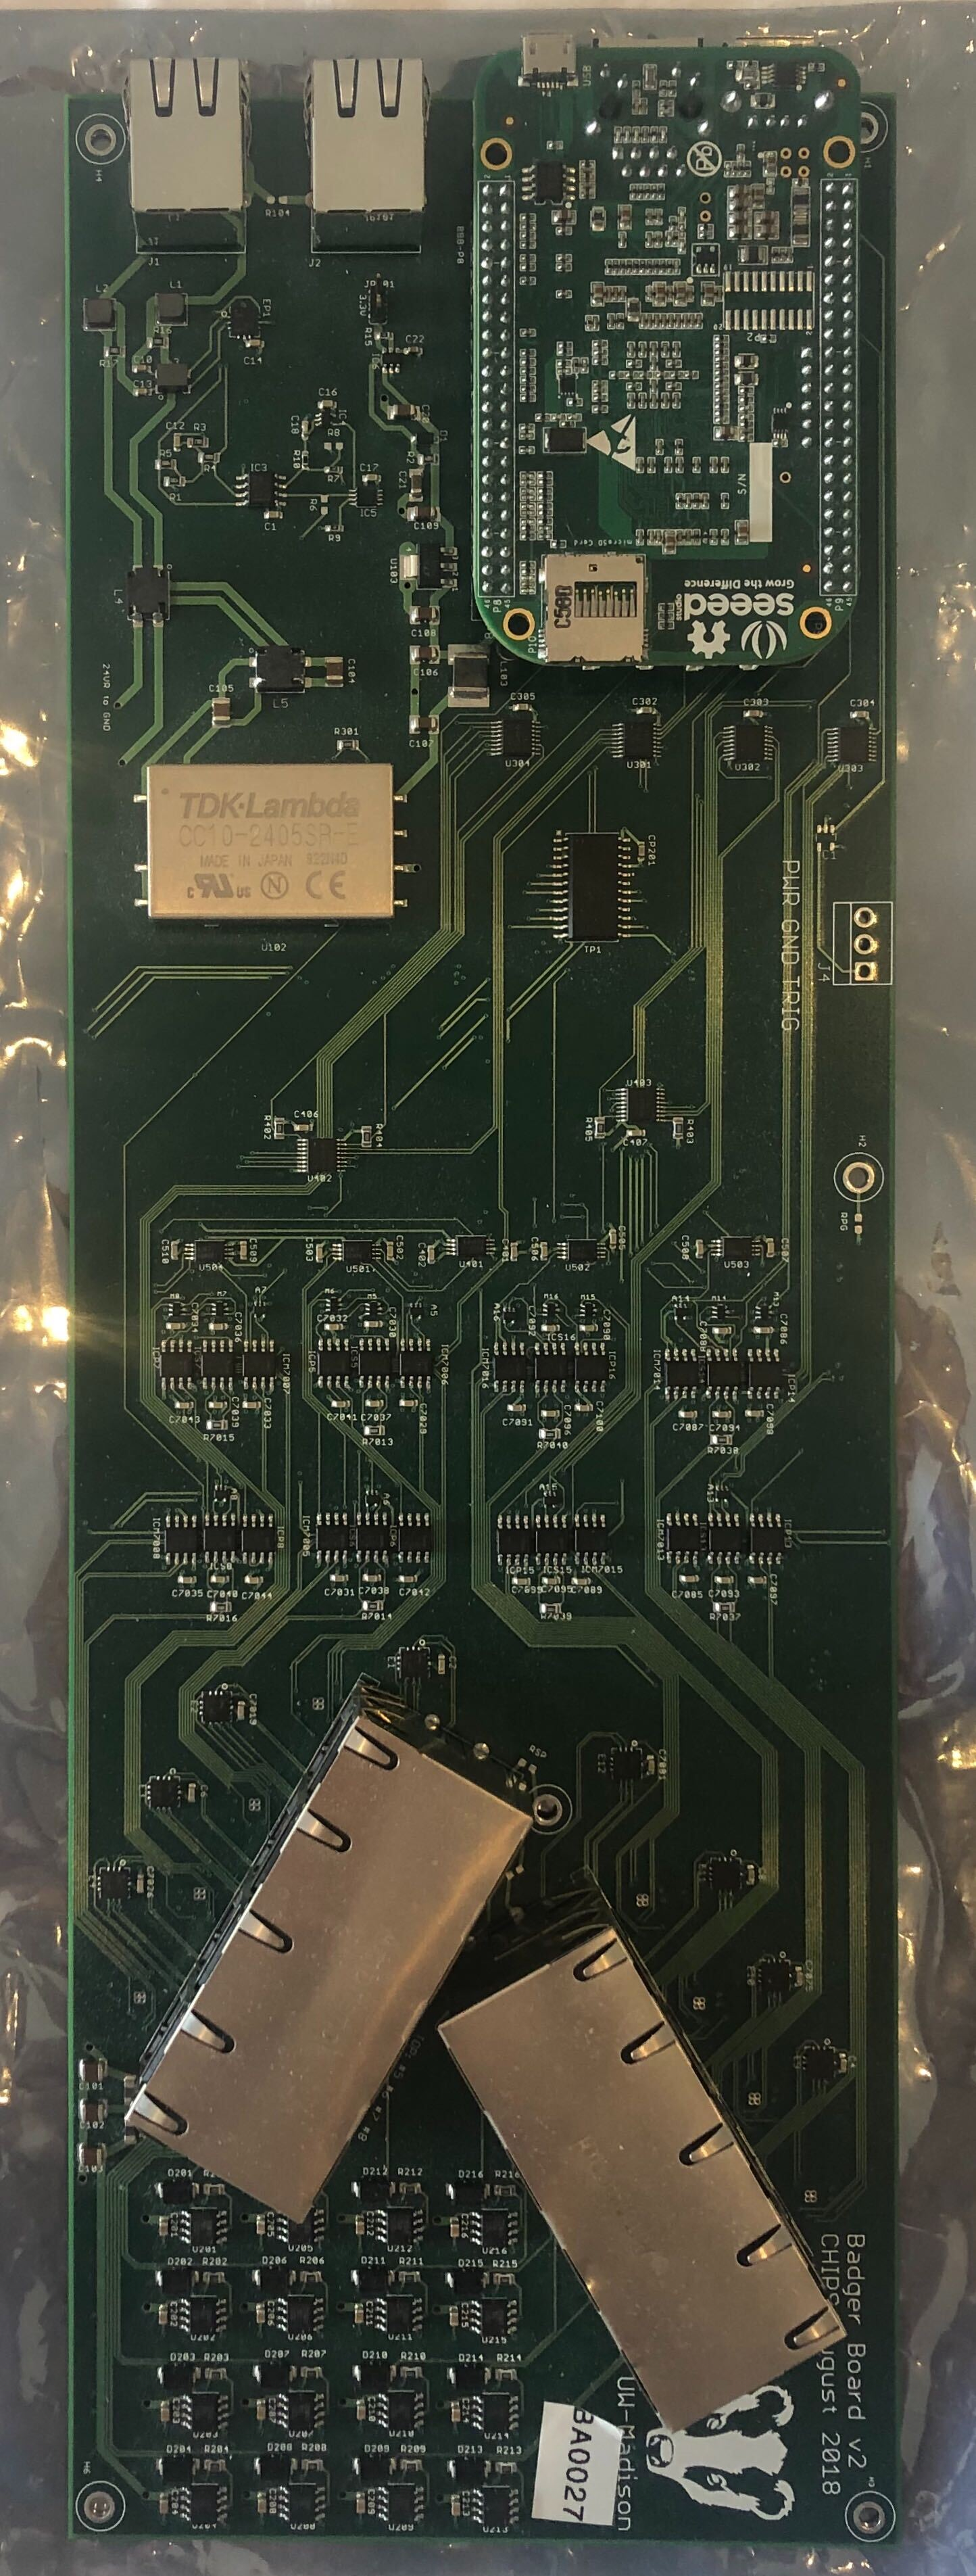
\includegraphics[angle=90,origin=c,width=0.8\textwidth]{diagrams/6-daq/badger.jpg}
    \caption[badger short]
    {badger long}
    \label{fig:badger}
\end{figure}

\subsection{Combined systems} %%%%%%%%%%%%%%%%%%%%%%%%%%%%%%%%%%%%%%%%%%%%%%%%%%%%%%%%%%%%%%%%%%%%
\label{sec:daq_hard_combined} %%%%%%%%%%%%%%%%%%%%%%%%%%%%%%%%%%%%%%%%%%%%%%%%%%%%%%%%%%%%%%%%%%%%

DIAGRAM: Hut Diagram + Jelly box diagram + EC diagrams
DIAGRAM: Manifold layout, box layout in detector

\begin{figure} % WHITE-RABBIT GM SETUP DIAGRAM %
    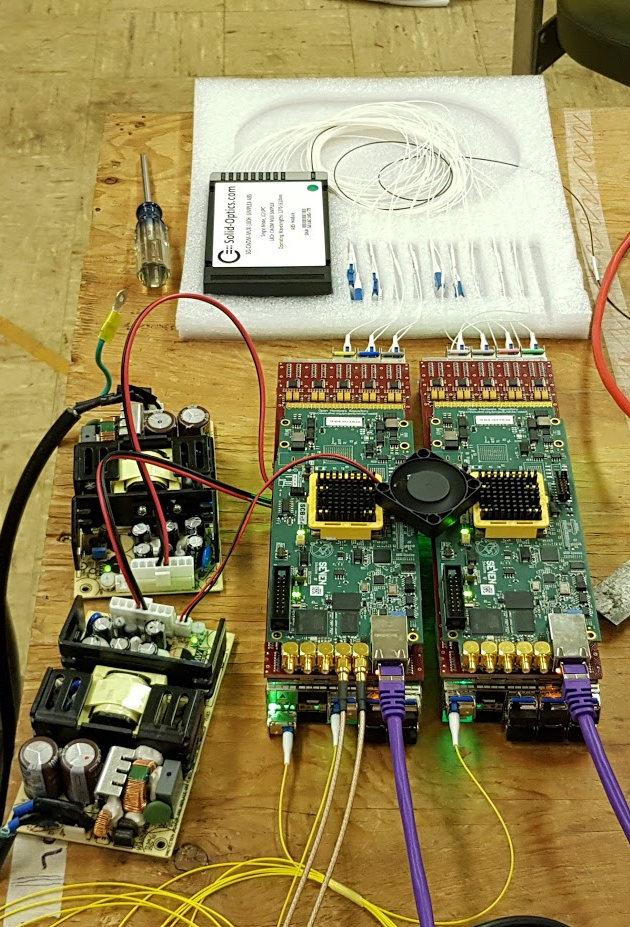
\includegraphics[width=0.8\textwidth]{diagrams/6-daq/wr_gm.jpg}
    \caption[wr gm short]
    {wr gm long}
    \label{fig:wr_gm}
\end{figure}

\section{Software} %%%%%%%%%%%%%%%%%%%%%%%%%%%%%%%%%%%%%%%%%%%%%%%%%%%%%%%%%%%%%%%%%%%%%%%%%%%%%%%
\label{sec:daq_soft} %%%%%%%%%%%%%%%%%%%%%%%%%%%%%%%%%%%%%%%%%%%%%%%%%%%%%%%%%%%%%%%%%%%%%%%%%%%%%

DIAGRAM: Software diagram
DIAGRAM: Finite state machine diagram

\subsection{The beam spill} %%%%%%%%%%%%%%%%%%%%%%%%%%%%%%%%%%%%%%%%%%%%%%%%%%%%%%%%%%%%%%%%%%%%%%
\label{sec:daq_soft_spill} %%%%%%%%%%%%%%%%%%%%%%%%%%%%%%%%%%%%%%%%%%%%%%%%%%%%%%%%%%%%%%%%%%%%%%%

DIAGRAM: Spill server/Fermilab diagram

\subsection{Hit acquisition and handling} %%%%%%%%%%%%%%%%%%%%%%%%%%%%%%%%%%%%%%%%%%%%%%%%%%%%%%%%
\label{sec:daq_soft_hits} %%%%%%%%%%%%%%%%%%%%%%%%%%%%%%%%%%%%%%%%%%%%%%%%%%%%%%%%%%%%%%%%%%%%%%%%

\subsection{Detector and data quality monitoring} %%%%%%%%%%%%%%%%%%%%%%%%%%%%%%%%%%%%%%%%%%%%%%%%
\label{sec:daq_soft_monitor} %%%%%%%%%%%%%%%%%%%%%%%%%%%%%%%%%%%%%%%%%%%%%%%%%%%%%%%%%%%%%%%%%%%%%

DIAGRAM: Monitoring diagram
REF: Elasticsearch paper

\begin{figure} % MONITORING DIAGRAM %
    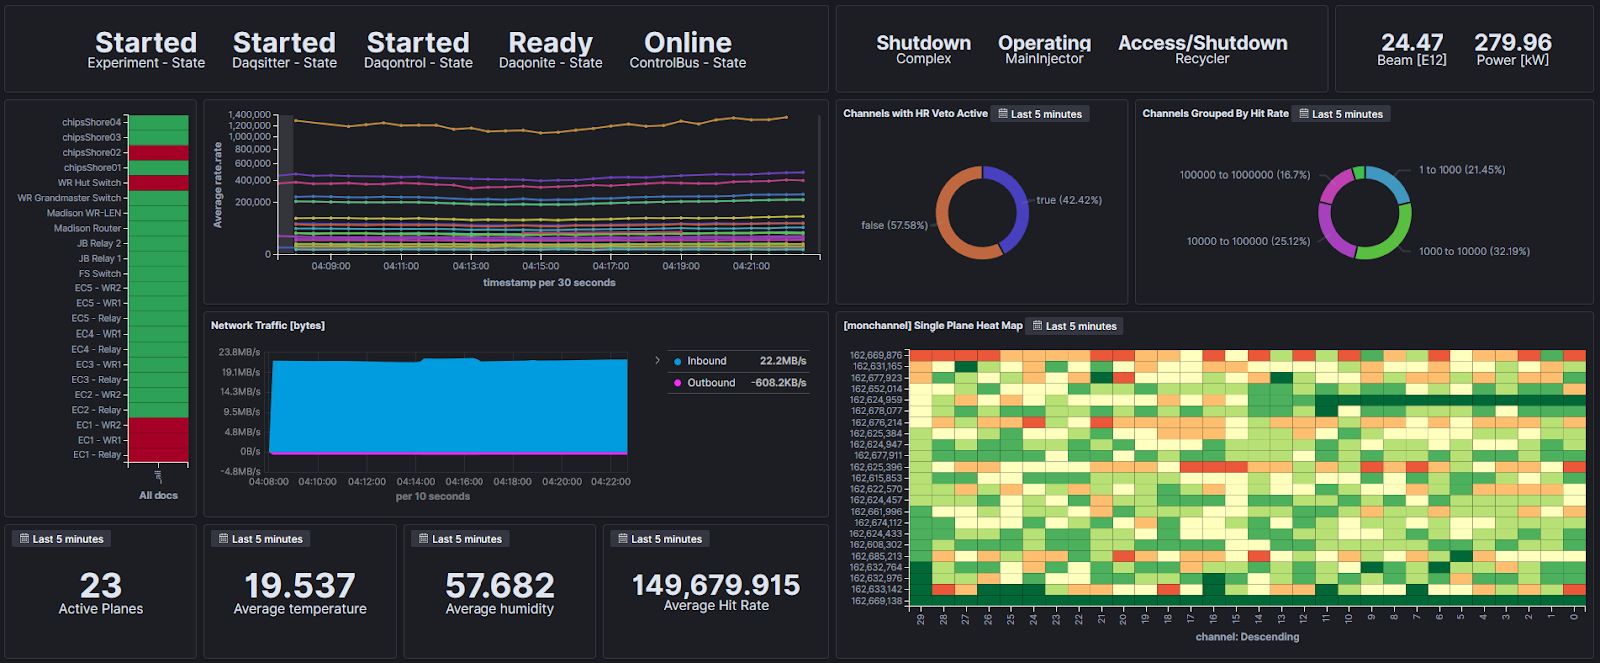
\includegraphics[width=\textwidth]{diagrams/6-daq/monitoring.png}
    \caption[monitoring short]
    {monitoring long}
    \label{fig:monitoring}
\end{figure}
    \chapter{A convolutional neural network for CHIPS} %%%%%%%%%%%%%%%%%%%%%%%%%%%%%%%%%%%%%%%%%%%%%%%
\label{chap:cvn} %%%%%%%%%%%%%%%%%%%%%%%%%%%%%%%%%%%%%%%%%%%%%%%%%%%%%%%%%%%%%%%%%%%%%%%%%%%%%%%%%

\begin{comment} % PLAN %%%%%%%%%%%%%%%%%%%%%%%%%%%%%%%%%%%%%%%%%%%%%%%%%%%%%%%%%%%%%%%%%%%%%%%%%%%
STORY OF THE CHAPTER There are many standard ways that event classification and paramter (mainly
energy) estimation are usually done in HEP. These mainly include the reconstruction of objects and
their associated parameters wether these are clusters, tracks, jets or cherenkov rings. Typically
these along with other constructed features are then passed through a simple machine learning
model for event or particle classification, or combined in some other way for energy estimation.

While this has worked leveraging the enormous amount of work in machine learning especially deep
learning surely would prove valuable. The key thing that has been done is to move away from human
engineered features to machine learning models that discover the underlying features that work
best in clasifiying of regressing a particualar task.

Water chernkov detectors are especially paired to this task as the output from our detectors is
essentially an 'image' of the event and so classification models that work well on images shoud
work well on seperating our types of events.

Firstly, the principle issue with matching water cherenkov detectors and deep learning is
representing the cylindrical detector output of either a 2d flat map that a typically conv network
can use as input of use a more complicated graph network approach as some other people have tried.
Typically people have just ignored the endcaps, but this is not optimal as these contain nearing
half the detected light in a standard CHIPS detector. Other appraoches include the x+ x- approach.
But as hited at by tomothy report, for a primarilly event classification task, removing any
distritions due to the detector shape is the most important things. Therefore, the approach of
veiwing the "image" from the interaction vertex point preserves the cherenkov ring strucutre as
best possible.

The hough space is used to find this vertex and direction from which the images are produces, so
it also made sense to include this along with time as a seperate channel in the output. You can
see
fro the vertext position is best. Using a more unformly distributes sample of events leads to a
greater abiity to distinguish the types which is important for subsequant energy reconstruction.

Many possible models have been developed for convolutional neural networks over th years.

Firstly, the principle issue with matching water cherenkov detectors and deep learning is
representing the cylindrical detector output of either a 2d flat map that a typically conv network
can use as input of use a more complicated graph network approach as some other people have tried.
Typically people have just ignored the endcaps, but this is not optimal as these contain nearing
half the detected light in a standard CHIPS detector. Other appraoches include the x+ x- approach.
But as hited at by tomothy report, for a primarilly event classification task, removing any
distritions due to the detector shape is the most important things. Therefore, the approach of
veiwing the "image" from the interaction vertex point preserves the cherenkov ring strucutre as
best possible.

INTRODUCTION
- Previous work etc...
- Previous applications in HEP

STANDARD RECONSTRUCTION METHODS
- Describe old likelihood based reconstruction (similar to fitqun)
- Describe standard MLP PID methods, hand engineered features etc...
- What are the main disadvantages of all of this?

THE THEORY OF DEEP CONVOLUTIONAL NEURAL NETWORKS
- How basic neural networks works
- How convolutional neural networks build onto of this
- How overfitting is prevented
- The evolutional of network structures

A BASELINE IMPLEMENTATION FOR CHIPS
- Tensorflow/python
- How the data flows
- Which architecture to use
- Which sample to use
- Which representation to use
- Multitask methodology

COSMIC REJECTION
- What is the scale of the task, the aim, expectations.
- How can we modify the baseline for cosmic rejection
- Does vertex help?
- Does escapes help?

BEAM CLASSIFICATION
- What is the scale of the task, the aim, expectations.
- How can we modify the baseline for beam classification
- What categorisation should we use?
- Does primary particle counting help?

ENERGY ESTIMATION
- What is the scale of the task, the aim, expectations.
- How can we modify the baseline for energy estimation.
- Should we learn an energy estimator for each event type?

FINAL PERFORMANCE
- Comparison with old reco/pid

EXPLAINABILITY
- t-SNE
- Lepton fraction energy performance
\end{comment}

\section{Introduction} %%%%%%%%%%%%%%%%%%%%%%%%%%%%%%%%%%%%%%%%%%%%%%%%%%%%%%%%%%%%%%%%%%%%%%%%%%%
\label{sec:cvn_intro} %%%%%%%%%%%%%%%%%%%%%%%%%%%%%%%%%%%%%%%%%%%%%%%%%%%%%%%%%%%%%%%%%%%%%%%%%%%%

- Explain the goals of both event reconstruction and event classification/ particle identification
- Main purpose for now is to allow for the exploration of different detector designs, for future
CHIPS detectors.

\subsection{Previous deep learning for neutrinos} %%%%%%%%%%%%%%%%%%%%%%%%%%%%%%%%%%%%%%%%%%%%%%%%
\label{sec:cvn_intro_previous} %%%%%%%%%%%%%%%%%%%%%%%%%%%%%%%%%%%%%%%%%%%%%%%%%%%%%%%%%%%%%%%%%%%

- Previous work in HEP has applied deep learning to a variety of problems...
- DUNE classifies neutrino ineractions in the DUNE FD using a CVN.
- DUNE uses 500*500 pixel images for each of the three readout views of the LArTPC.
- They just uses events with vertex within the detector iducial volume.
- Events that contain < 10 non-zero pixels are removed, similar to my removal of low hit events.
- They use a SE-ResNet architecture, with three branches for each inut view that are then
concatenated for the deeper layers of the network.
- They do multi-task learning, with 7 tasks.
- Trained on MC sample of events for the DUNE unosicllated FD neutrino event rate distribution.

Cern summer report in Ref.~\cite{theodore2016}
Nova first CVN paper in Ref.~\cite{aurisano2016}
Nova context enriched CVN paper in Ref.~\cite{psihas2019}
Nova energy recontruction CVN in Ref.~\cite{baldi2019}
MicroBooNE CNN paper in Ref.~\cite{acciarri2017}
Watchmal/Triumf Cherenkov variational autoencoders in Ref.~\cite{abhishek2019}
Daya bay paper in Ref.~\cite{racah2016}
SHiP GAN simulation paper in Ref.~\cite{ahdida2019}
DUNE CVN paper in Ref.~\cite{collaboration2020}
DUNE TDR in Ref.~\cite{abi2020}

\section{Standard reconstruction and particle identification} %%%%%%%%%%%%%%%%%%%%%%%%%%%%%%%%%%%%
\label{sec:cvn_old} %%%%%%%%%%%%%%%%%%%%%%%%%%%%%%%%%%%%%%%%%%%%%%%%%%%%%%%%%%%%%%%%%%%%%%%%%%%%%%

It is important to outline the standard event reconstruction and particle identification methods
thats have been used by the \chips project up till now. This is key for two reasons. Firstly, to
add context for the performance comparison with the new convolutional neural network approach
later in the chapter. Secondly, the highlight the main weaknesses of these methods, motivating the
need for the new technique and making its advantages clear.

A maximum likelihood method based on that implemented by MiniBooNE~\cite{patterson2009} is used
for event reconstruction. Additionally, an artificial neural network built using the TMVA
package~\cite{hocker2007} and using outputs from the reconstruction is used for particle
identification. Both methods are very typical of the `mainstream' approach used by the majority of
water Cherenkov neutrino experiments. A prime example is the fiTQun algorithm developed for the
Super-Kamiokande detector, which is now used for both atmospheric~\cite{jiang2019} and
T2K~\cite{missert2017} analyses.

Due to the small size and limited resources of the \chips project collaboration it is highly
likely that both the event recontruction and particle identification do not represent the
`optimal' implementation of these methods. However, through tracking the development process of
both methods it is clear that any performance improvements would now be small relative to those
introduced by the new convolutional neural network approach. Thus, it can be assumed that
the implementation approximates the maximum performance these approaches can provide reasonably
well.

\section{Likelihood based reconstruction} %%%%%%%%%%%%%%%%%%%%%%%%%%%%%%%%%%%%%%%%%%%%%%%%%%%%%%%%
\label{sec:cvn_old_reco} %%%%%%%%%%%%%%%%%%%%%%%%%%%%%%%%%%%%%%%%%%%%%%%%%%%%%%%%%%%%%%%%%%%%%%%%%

The first stage of event reconstruction is seeding, which attempts to make a reasonable `guess' at
the event track parameters before the full likelihood based method is used. After seperating hits
in space and time and applying basic filtering to remove outlying hits, a series of vertexing
algorithms estimate the interaction vertex position, time and initial track direction.

- First stage is track seeding, which attempts to make a reasonable "guess" at the track
parameters before the likelihood based minimisation methods begins.
- Hits are firstly seperated in space and time and basic filtering is applied to remove outliying
hits not clearly associated with a region of interest.
- A series of vertexing algorithsm are applied to produce an estimate of the interaction vertex
position, time and track direction.
- These are then used in a hough transform algorithm to refine to track direction values and to
look for sub-dominant directions that could indicate multiple particles causing the energy
deposits.
- The output from the seeding process is a list of seeds where each seed is an initial guess
at the track parameters exluding the energy which is not estimated by the seeding algorithms.
- The seeds are oredered by their peak height in the hough transform space, with a greater height
indicating a more likely seed.
- Multiple track hypothesis to use in the likelihood method can then be seeded from the list in
decending order.

- Standard water cherenkov analysis is via a likelihood hood fit to the ring assuming some event
topology hypothesis.
- This is used in super-k with fitqun and what has been previously implemented for CHIPS in the
WCSimAnalysis package.
- BAsed on calculating the likelihood to observe energy deposits of a given charge and time for
a particular particle track hypothesis.
- very relient on the hypothesis, in reality the majority of interactions are not simple single
track events, so this quickly becomes difficult.
- Based n the likelihood methods developed for MiniBooNE experiment.
- Given a hypothesised set of tracks, the number of photoelectrons and the time at which the
first electron is detected for each PMT within the detector is predicted.
- By comparison with the measured hit charges and times for the event, the likelihood that the
given track hypothesis produced the measured signals is calculated.
- The track paramaters are then varied until the negative logarithm of the likelihood is minimised
This then indicates the best-fit track hypothesis to the measurements.
- Note: this is heavily dependent on what track hypothesis is made. Is it a single particle, two
overlapping particles?
- Goes through multiple stages of fitting, freeing and fixing certain parameters to reach the
optimised track paramter solution.

- Note: each likelihood minimisation takes approx 2mins to run on a standard computing node.

- CHIPS reco paper~\cite{blake2016}
- MiniBooNE track reconstruction~\cite{patterson2009}
- Super-k fitqun usage~\cite{jiang2019}
- T2K fitqun usage~\cite{missert2017}

\begin{equation} % LIKELIHOOD EQUATION %
    \mathcal{L}(x)=\mathcal{L}_{unhit}(x)\mathcal{L}_{hit}(x)=\prod_{unhit}P_{unhit}(x)
    \prod_{hit}P_{charge}(x)P_{time}(x)
\end{equation}

\begin{itemize}
    \item Track vertex position ($x_{0}$,$y_{0}$,$z_{0}$) and interaction time $t_{0}$
    \item Initial track direction ($d_{x}$,$d_{y}$,$d_{z}$)
    \item Initial kinetic energy of the particle
    \item Particle type (muon, electron or photon)
\end{itemize}


\section{Particle identification} %%%%%%%%%%%%%%%%%%%%%%%%%%%%%%%%%%%%%%%%%%%%%%%%%%%%%%%%%%%%%%%%
\label{sec:cvn_old_pid} %%%%%%%%%%%%%%%%%%%%%%%%%%%%%%%%%%%%%%%%%%%%%%%%%%%%%%%%%%%%%%%%%%%%%%%%%%

- TMVA paper~\cite{hocker2007}
- ROOT paper~\cite{brun1997}

\begin{itemize}
    \item $\Delta\ln\mathcal{L}$ between electron and muon hypothesis for both time and charge
          components
    \item The number of hit PMTs ($N_{hits}$)
    \item $\frac{\Delta\ln\mathcal{L}_{charge}}{N_{hits}}$
    \item Fraction of hits inside, within and outside the central hole of the ring for
          both electron and muon hypotheses
    \item Fraction of predicted charge outside the ring for both electron and muon hypotheses
    \item Ratio of the total predicted charged to the total measured charge for both electron
          and muon hypothesis
    \item The ratio of the reconstructed energy to the total measured charge
    \item Reconstructed track direction under the electron hypothesis
    \item Fraction of hits in the downstream half of the detector

    \item Number of seeds generated by the hough transform seeding algorithm
    \item Peak height of the first and last seeds found by the hough transform seeding algorithm.
\end{itemize}

- Primarily driven by the difference in the log likelihood between the different likelihood
hypotheses for an event.
- Two artifical neural networks (ANNs) were developed, The first is used to seperate electon-like
from muon-like interactions and the second to seperate between electron-like and NC interactions.
- Trained on a sample of beam events

- These are all hand engineered features, found by trial and error by a human. They are ofcourse
physically motivate to some degree, and would be expected to be different for different categories
of event to discriminate between them.
- It's very unlikely this is firstly and exhaustive list of all features that could be used, or
that these are the best features to use.
- Very hard when the parameter space of possible discriminating engineered features is so large.


\section{The theory of deep convolutional neural networks} %%%%%%%%%%%%%%%%%%%%%%%%%%%%%%%%%%%%%%%
\label{sec:cvn_theory} %%%%%%%%%%%%%%%%%%%%%%%%%%%%%%%%%%%%%%%%%%%%%%%%%%%%%%%%%%%%%%%%%%%%%%%%%%%

\subsection{Neural networks} %%%%%%%%%%%%%%%%%%%%%%%%%%%%%%%%%%%%%%%%%%%%%%%%%%%%%%%%%%%%%%%%%%%%%
\label{sec:cvn_theory_basic} %%%%%%%%%%%%%%%%%%%%%%%%%%%%%%%%%%%%%%%%%%%%%%%%%%%%%%%%%%%%%%%%%%%%%

Amazing machine learning for physicists thing in Ref.~\cite{mehta2019}

\begin{equation} % NETWORK BASIC EQUATION %
    z^{(i)}=\boldsymbol{w}^{(i)}\cdot\boldsymbol{x}+b^{(i)}
\end{equation}

\begin{equation} % NETWORK ACTIVATION EQUATION %
    a_{i}(\boldsymbol{x})=\sigma_i(z^{(i)})
\end{equation}

\begin{figure} % BASIC NETWORK DIAGRAM %
    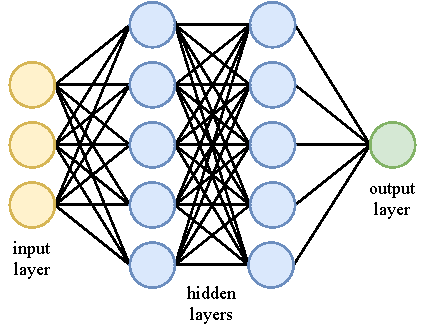
\includegraphics[width=0.8\textwidth]{diagrams/7-cvn/network.pdf}
    \caption[network short]
    {network long}
    \label{fig:network}
\end{figure}

\begin{equation} % MEAN-SQUARED ERROR LOSS EQUATION %
    E(\boldsymbol{w})=
    \frac{1}{n}\displaystyle\sum_{i=1}^{n}(y_{i}-
    \hat{y}_{i}(\boldsymbol{w}))^{2}
\end{equation}

\begin{equation} % BINARY CROSS-ENTROPY EQUATION %
    E(\boldsymbol{w})=
    -\displaystyle\sum_{i=1}^{n}y_{i}\log\hat{y}_{i}(\boldsymbol{w})+
    (1-y_{i})\log[1-\hat{y}_{i}(\boldsymbol{w})]
\end{equation}

\begin{equation} % CATEGORICAL CROSS-ENTROPY EQUATION %
    E(\boldsymbol{w})=
    -\displaystyle\sum_{i=1}^{n}\displaystyle\sum_{m=0}^{M-1}y_{im}\log\hat{y}_{im}
    (\boldsymbol{w})+(1-y_{im})\log[1-\hat{y}_{im}(\boldsymbol{w})]
\end{equation}

\subsection{Convolutional neural networks} %%%%%%%%%%%%%%%%%%%%%%%%%%%%%%%%%%%%%%%%%%%%%%%%%%%%%%%
\label{sec:cvn_theory_conv} %%%%%%%%%%%%%%%%%%%%%%%%%%%%%%%%%%%%%%%%%%%%%%%%%%%%%%%%%%%%%%%%%%%%%%

EQUATION: Back propogation equations derivation and explanation

\begin{figure} % ACTIVATIONS DIAGRAM %
    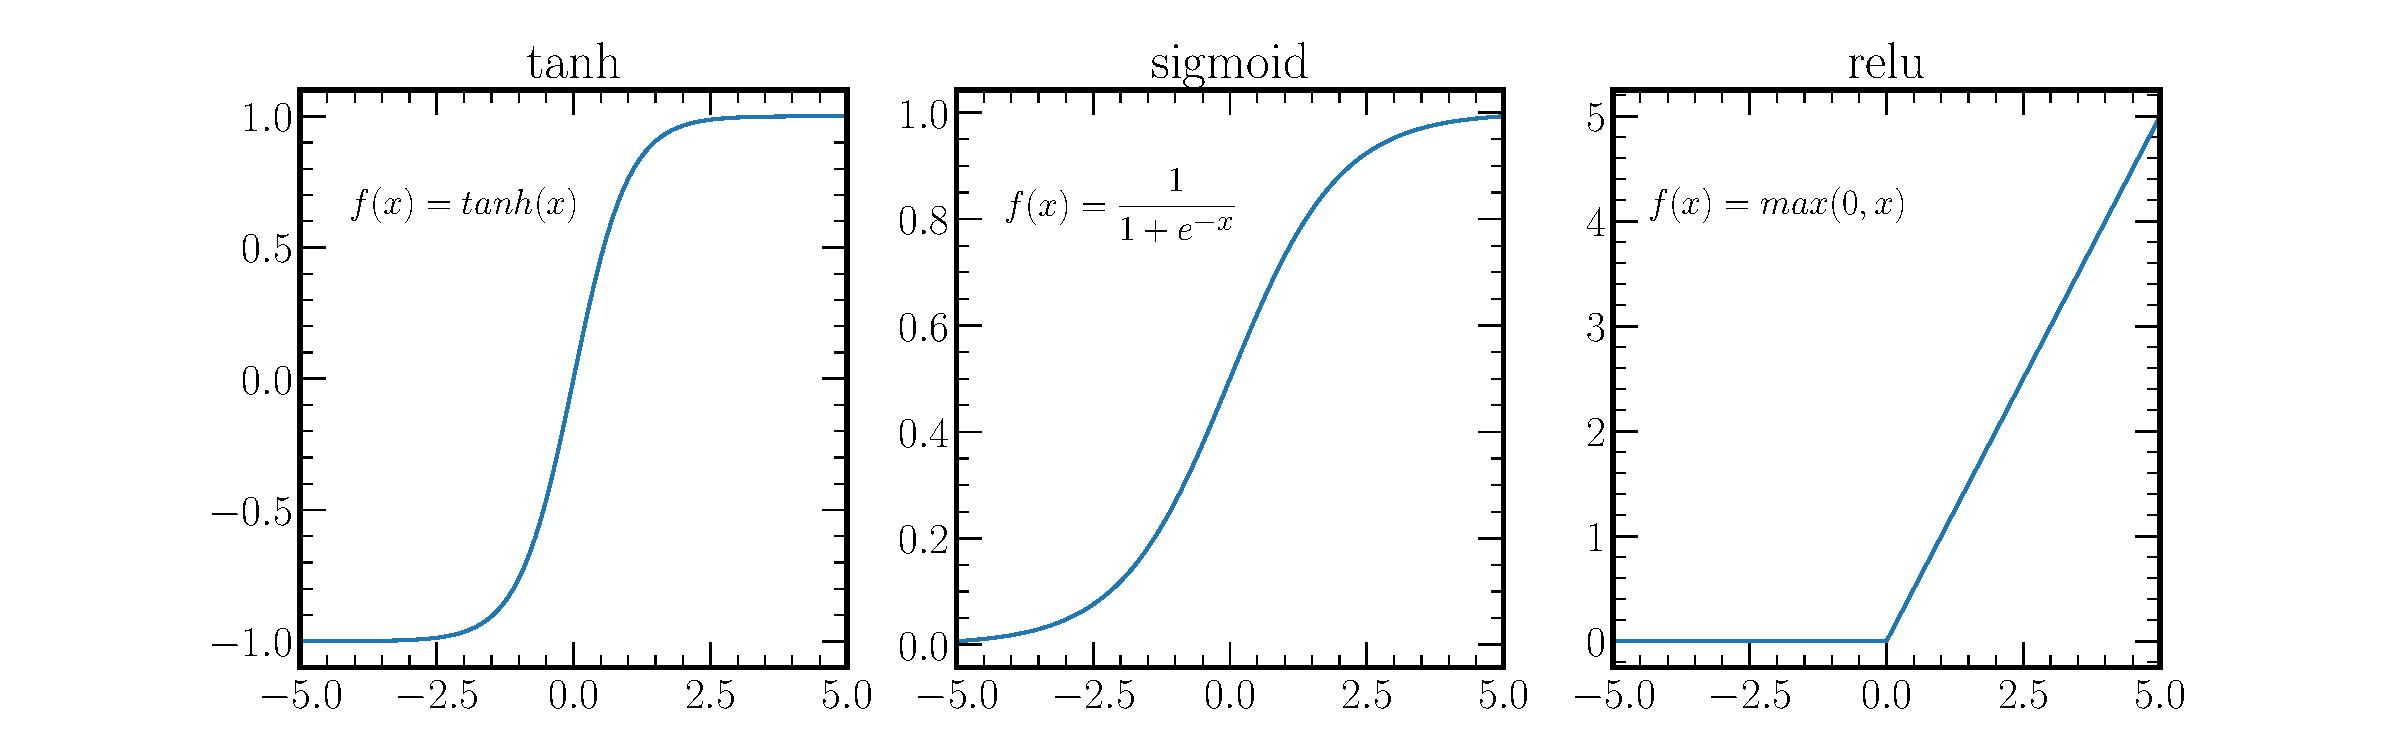
\includegraphics[width=\textwidth]{diagrams/7-cvn/activations.pdf}
    \caption[activations short]
    {activations long}
    \label{fig:activations}
\end{figure}

\begin{figure} % GRADIENT DESCENT DIAGRAM %
    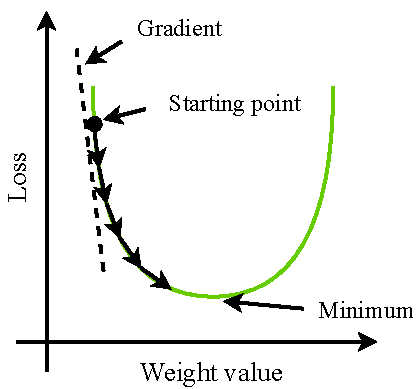
\includegraphics[width=0.8\textwidth]{diagrams/7-cvn/gradient_descent.pdf}
    \caption[gradient descent short]
    {gradient descent long}
    \label{fig:gradient_descent}
\end{figure}

\begin{figure} % CONV INPUTS DIAGRAM %
    \centering
    \begin{subfigure}[b]{0.4\textwidth}
        \centering
        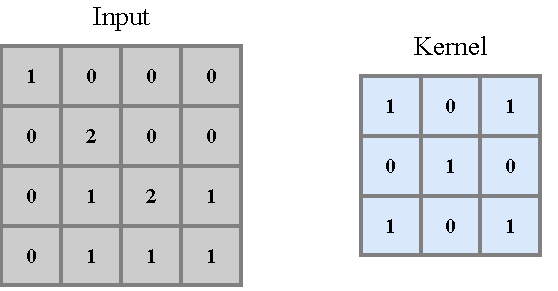
\includegraphics[width=\textwidth]{diagrams/7-cvn/conv_input.pdf}
        \caption{conv input long}
        \label{fig:conv_input}
    \end{subfigure}
    \hfill
    \begin{subfigure}[b]{0.4\textwidth}
        \centering
        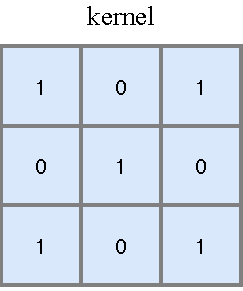
\includegraphics[width=\textwidth]{diagrams/7-cvn/conv_kernel.pdf}
        \caption{conv kernel long}
        \label{fig:conv_kernel}
    \end{subfigure}
    \caption{conv input and kernel}
    \label{fig:conv_input_kernel}
\end{figure}

TODO: combine the same and valid conv operations into the same diagram

\begin{figure} % CONV OPERATION DIAGRAM %
    \centering
    \begin{subfigure}[b]{0.71\textwidth}
        \centering
        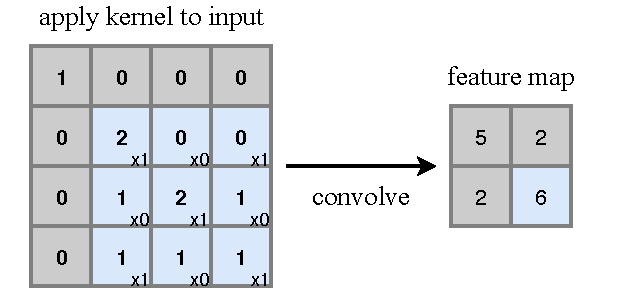
\includegraphics[width=\textwidth]{diagrams/7-cvn/conv_valid.pdf}
        \caption{conv valid long}
        \label{fig:conv_valid}
    \end{subfigure}
    \hfill
    \begin{subfigure}[b]{0.9\textwidth}
        \centering
        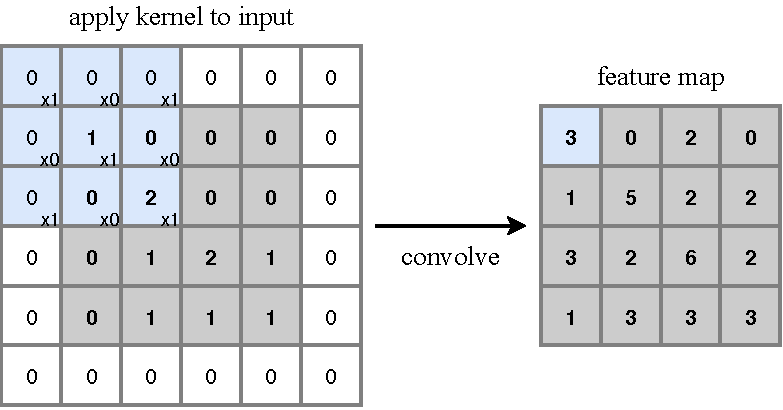
\includegraphics[width=\textwidth]{diagrams/7-cvn/conv_same.pdf}
        \caption{conv same long}
        \label{fig:conv_same}
    \end{subfigure}
    \caption{conv operations}
    \label{fig:conv_operations}
\end{figure}

\begin{figure} % POOLING DIAGRAM %
    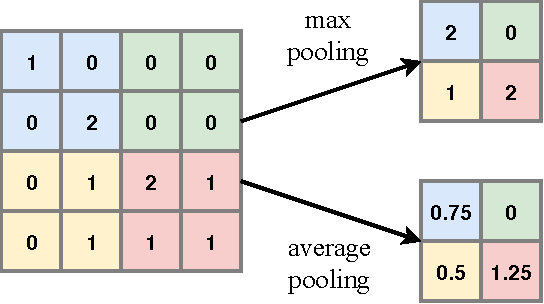
\includegraphics[width=0.8\textwidth]{diagrams/7-cvn/pooling.pdf}
    \caption[pooling short]
    {pooling long}
    \label{fig:pooling}
\end{figure}

\subsection{The evolution of convolutional networks} %%%%%%%%%%%%%%%%%%%%%%%%%%%%%%%%%%%%%%%%%%%%%
\label{sec:cvn_theory_architectures} %%%%%%%%%%%%%%%%%%%%%%%%%%%%%%%%%%%%%%%%%%%%%%%%%%%%%%%%%%%%%

Original 'dropout' paper in Ref.~\cite{hinton2012}
Original Batch normalisation paper in Ref.~\cite{ioffe2015}
Bag of tricks in Ref.~\cite{he2018}
VGG paper in Ref.~\cite{simonyan2014}
Improved resnet paper in Ref.~\cite{he2016}
Inception-resnet paper in Ref.~\cite{szegedy2016}
Squeeze-and-excitation networks paper in Ref.~\cite{hu2017}
MobileNetV2 paper in Ref.~\cite{sandler2018}
EfficientNet paper in Ref.~\cite{tan2019}

EQUATION: Batch-normalisation equations

\begin{figure} % DROPOUT DIAGRAM %
    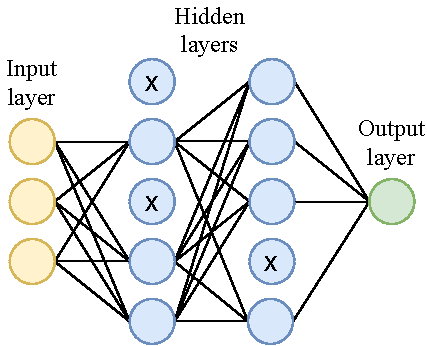
\includegraphics[width=0.8\textwidth]{diagrams/7-cvn/dropout.pdf}
    \caption[dropout short]
    {dropout long}
    \label{fig:dropout}
\end{figure}

\begin{figure} % EARLY STOPPING DIAGRAM %
    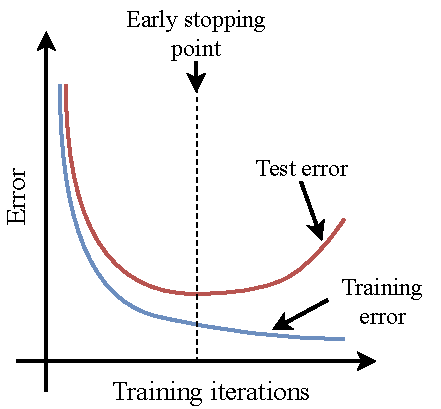
\includegraphics[width=0.8\textwidth]{diagrams/7-cvn/early_stopping.pdf}
    \caption[early stopping short]
    {early stopping long}
    \label{fig:early_stopping}
\end{figure}

\begin{figure} % SQUEEZE-EXITATION BLOCK DIAGRAM %
    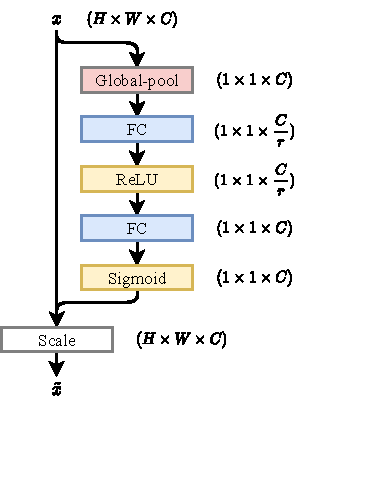
\includegraphics[width=0.8\textwidth]{diagrams/7-cvn/se.pdf}
    \caption[se short]
    {se long}
    \label{fig:se}
\end{figure}

\begin{figure} % RESNET BLOCK DIAGRAM %
    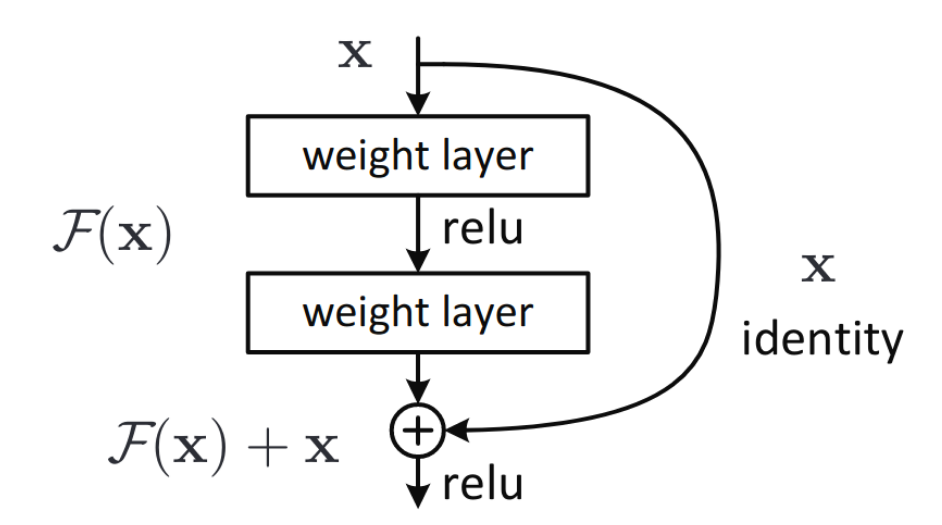
\includegraphics[width=0.8\textwidth]{diagrams/7-cvn/resnet_unit.png}
    \caption[resnet unit short]
    {resnet unit long}
    \label{fig:resnet_unit}
\end{figure}

\begin{figure} % INCEPTION BLOCK DIAGRAM %
    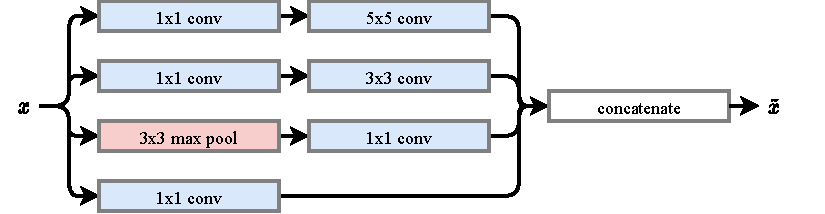
\includegraphics[width=0.8\textwidth]{diagrams/7-cvn/inception.pdf}
    \caption[inception short]
    {inception long}
    \label{fig:se}
\end{figure}

\section{A baseline implementation for CHIPS} %%%%%%%%%%%%%%%%%%%%%%%%%%%%%%%%%%%%%%%%%%%%%%%%%%%%
\label{sec:cvn_baseline} %%%%%%%%%%%%%%%%%%%%%%%%%%%%%%%%%%%%%%%%%%%%%%%%%%%%%%%%%%%%%%%%%%%%%%%%%

\begin{figure} % CHIPSNET DIAGRAM %
    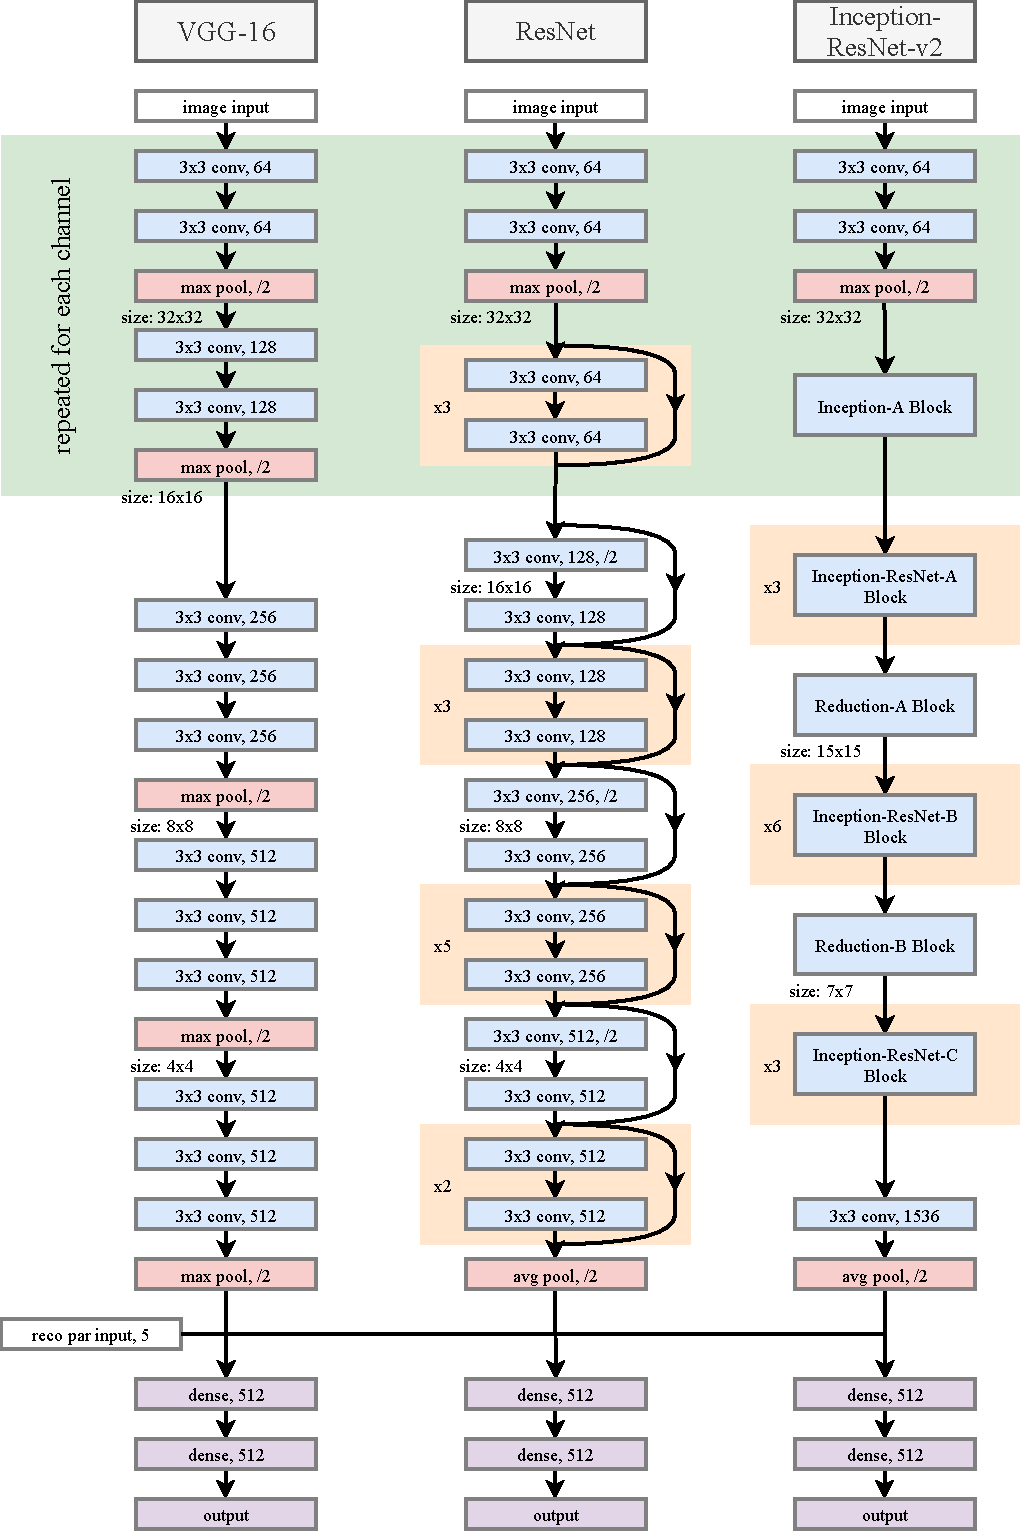
\includegraphics[width=0.8\textwidth]{diagrams/7-cvn/chipsnet.pdf}
    \caption[chipsnet short]
    {chipsnet long}
    \label{fig:chipsnet}
\end{figure}

\subsection{Software implementation} %%%%%%%%%%%%%%%%%%%%%%%%%%%%%%%%%%%%%%%%%%%%%%%%%%%%%%%%%%%%%
\label{sec:cvn_baseline_soft} %%%%%%%%%%%%%%%%%%%%%%%%%%%%%%%%%%%%%%%%%%%%%%%%%%%%%%%%%%%%%%%%%%%%

- Early stopping
- Model (dropout, batch norm, se, vgg etc...)

\begin{figure} % 8-BIT DIAGRAM %
    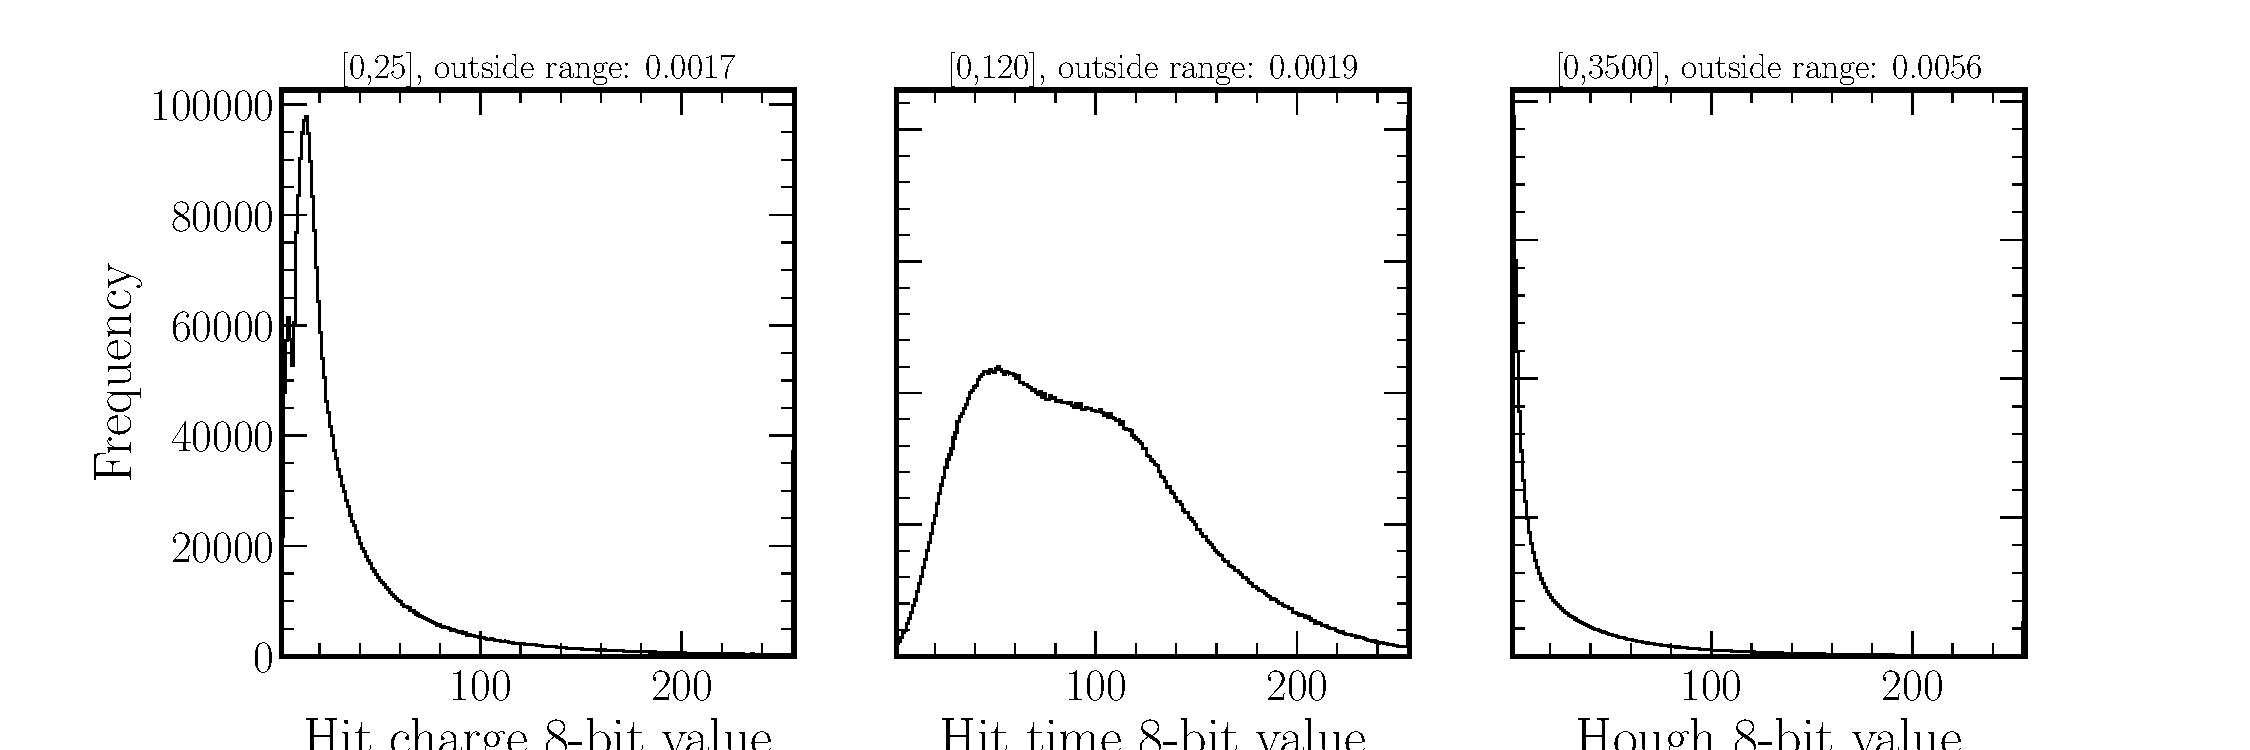
\includegraphics[width=\textwidth]{diagrams/7-cvn/chipsnet/expore_8_bit_range.pdf}
    \caption[explore 8 bit range short]
    {explore 8 bit range long}
    \label{fig:explore_8_bit_range}
\end{figure}

\subsection{Network architecture} %%%%%%%%%%%%%%%%%%%%%%%%%%%%%%%%%%%%%%%%%%%%%%%%%%%%%%%%%%%%%%%%
\label{sec:cvn_baseline_architecture} %%%%%%%%%%%%%%%%%%%%%%%%%%%%%%%%%%%%%%%%%%%%%%%%%%%%%%%%%%%%

\subsection{Which training sample to use} %%%%%%%%%%%%%%%%%%%%%%%%%%%%%%%%%%%%%%%%%%%%%%%%%%%%%%%%
\label{sec:cvn_baseline_sample} %%%%%%%%%%%%%%%%%%%%%%%%%%%%%%%%%%%%%%%%%%%%%%%%%%%%%%%%%%%%%%%%%%

\subsection{Which event representation to use} %%%%%%%%%%%%%%%%%%%%%%%%%%%%%%%%%%%%%%%%%%%%%%%%%%%
\label{sec:cvn_baseline_repr} %%%%%%%%%%%%%%%%%%%%%%%%%%%%%%%%%%%%%%%%%%%%%%%%%%%%%%%%%%%%%%%%%%%%

- Cern summer report in Ref.~\cite{theodore2016}
- New ideas with x+ x- mapping in Ref.~\cite{berns2020}

\begin{figure} % NUEL CCQEL EVENT DIAGRAM %
    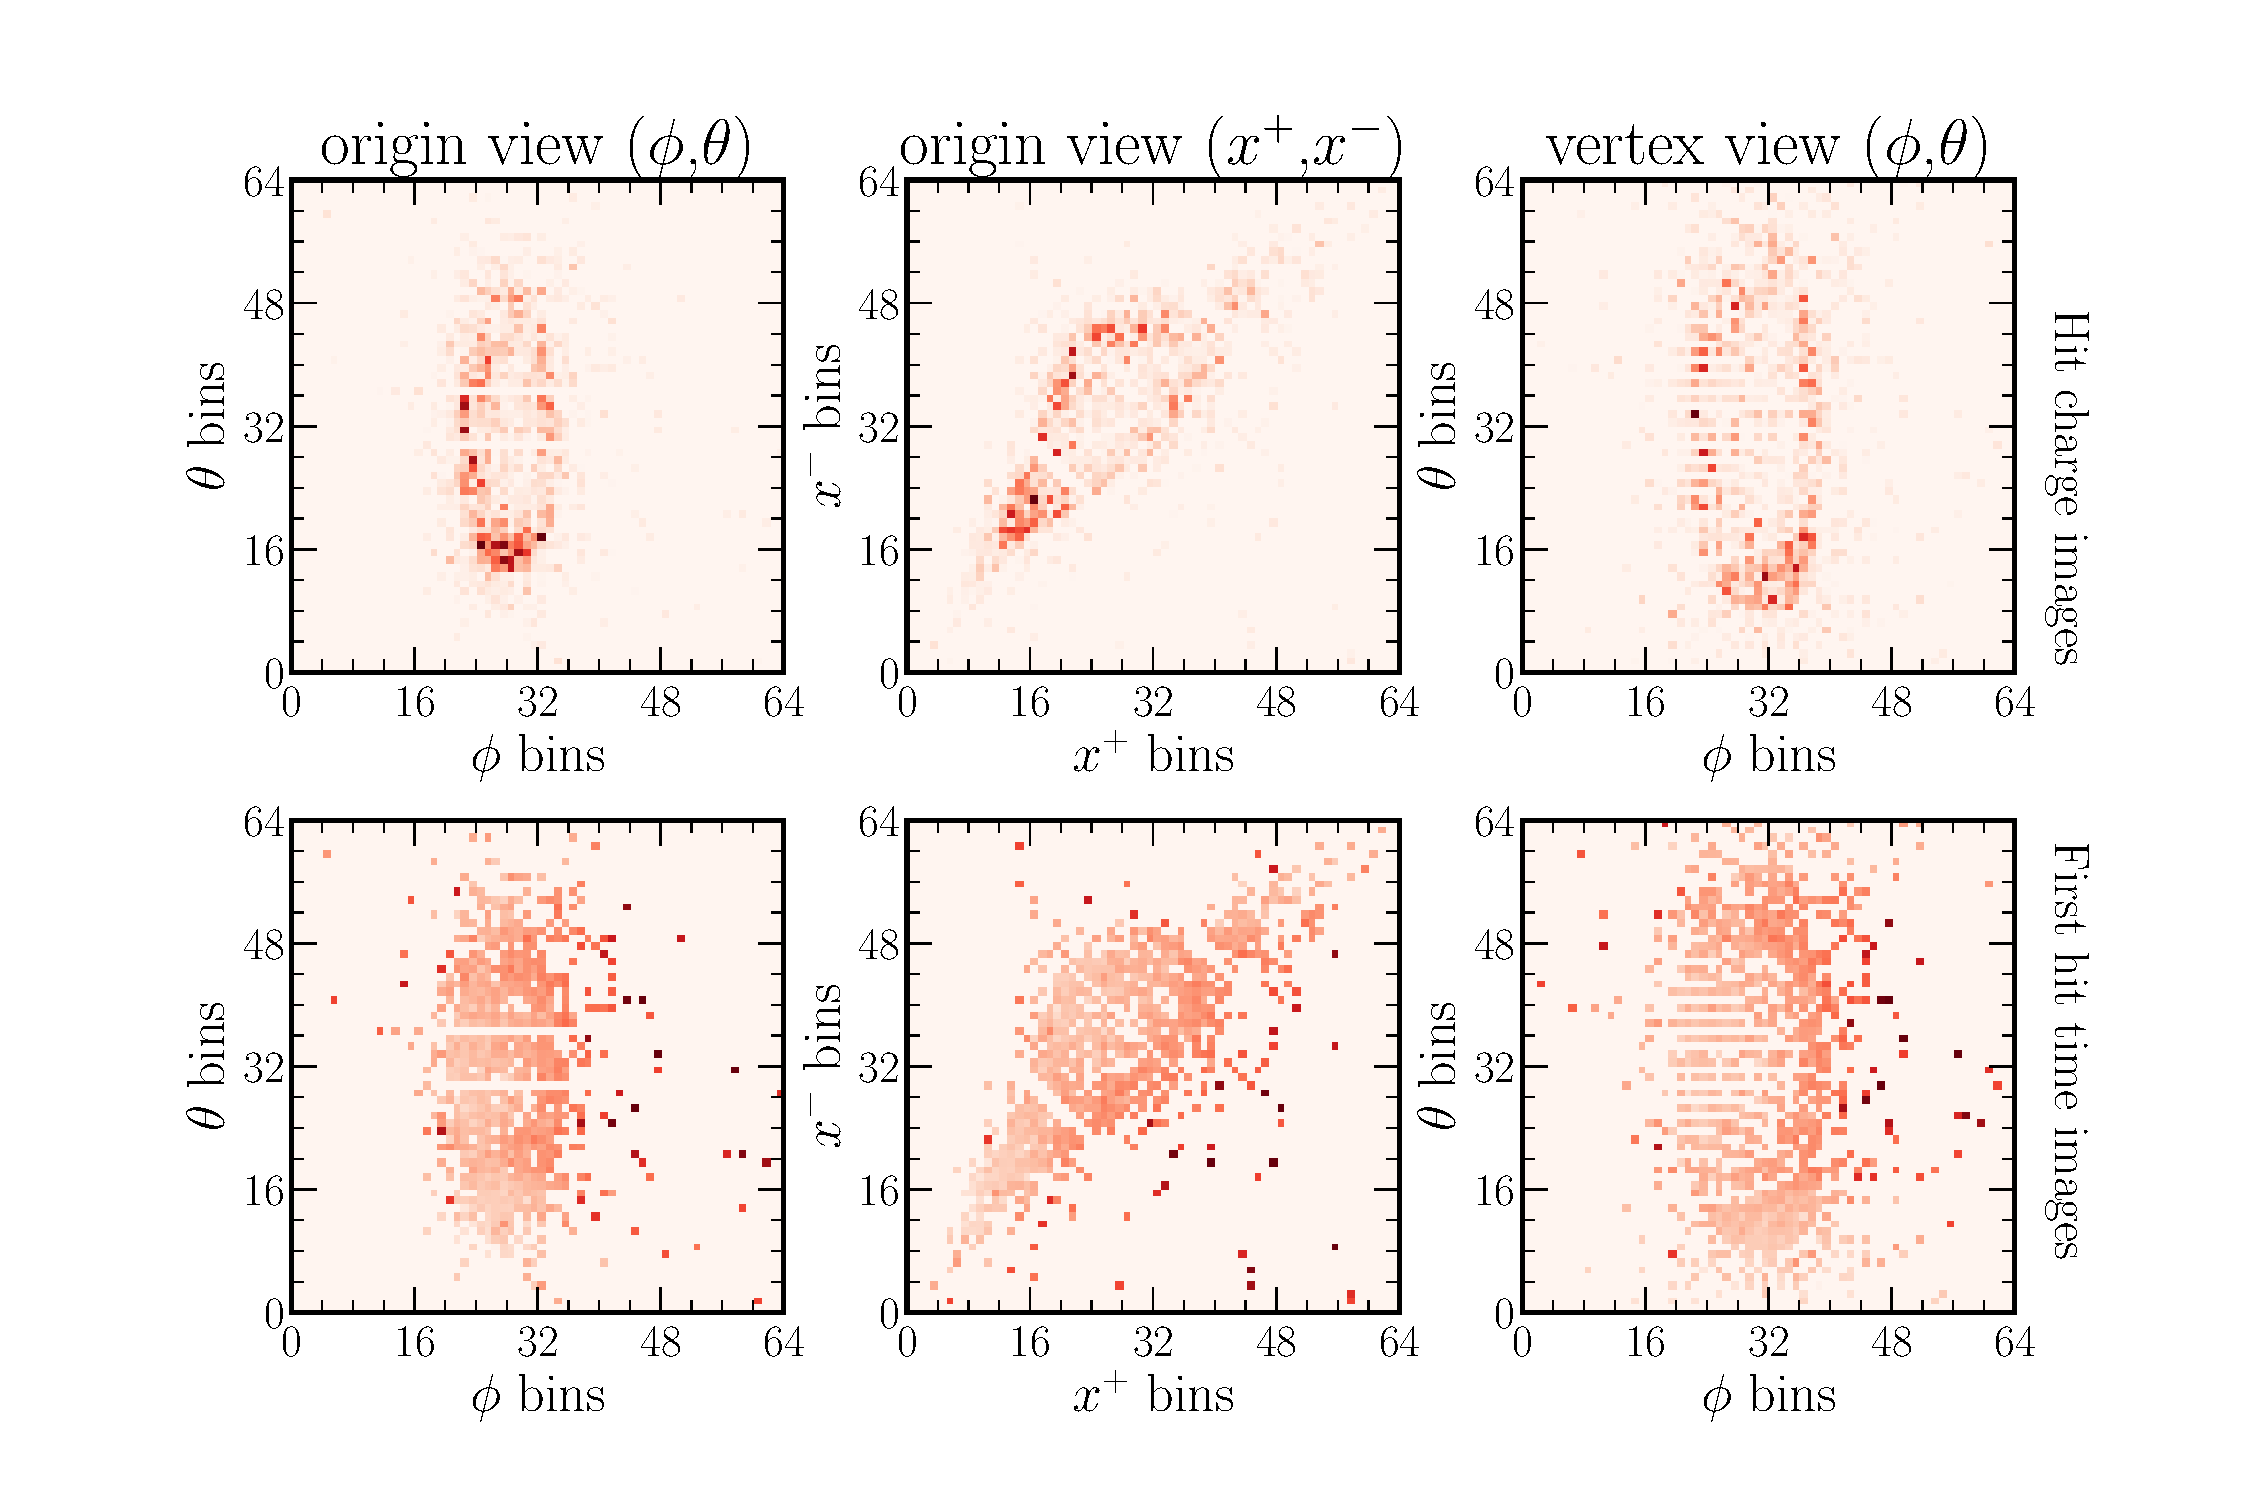
\includegraphics[width=\textwidth]{diagrams/7-cvn/chipsnet/explore_nuel_ccqel_event.pdf}
    \caption[explore nuel ccqel event short]
    {explore nuel ccqel event long}
    \label{fig:explore_nuel_ccqel_event}
\end{figure}

\begin{figure} % NUMU CCDIS EVENT DIAGRAM %
    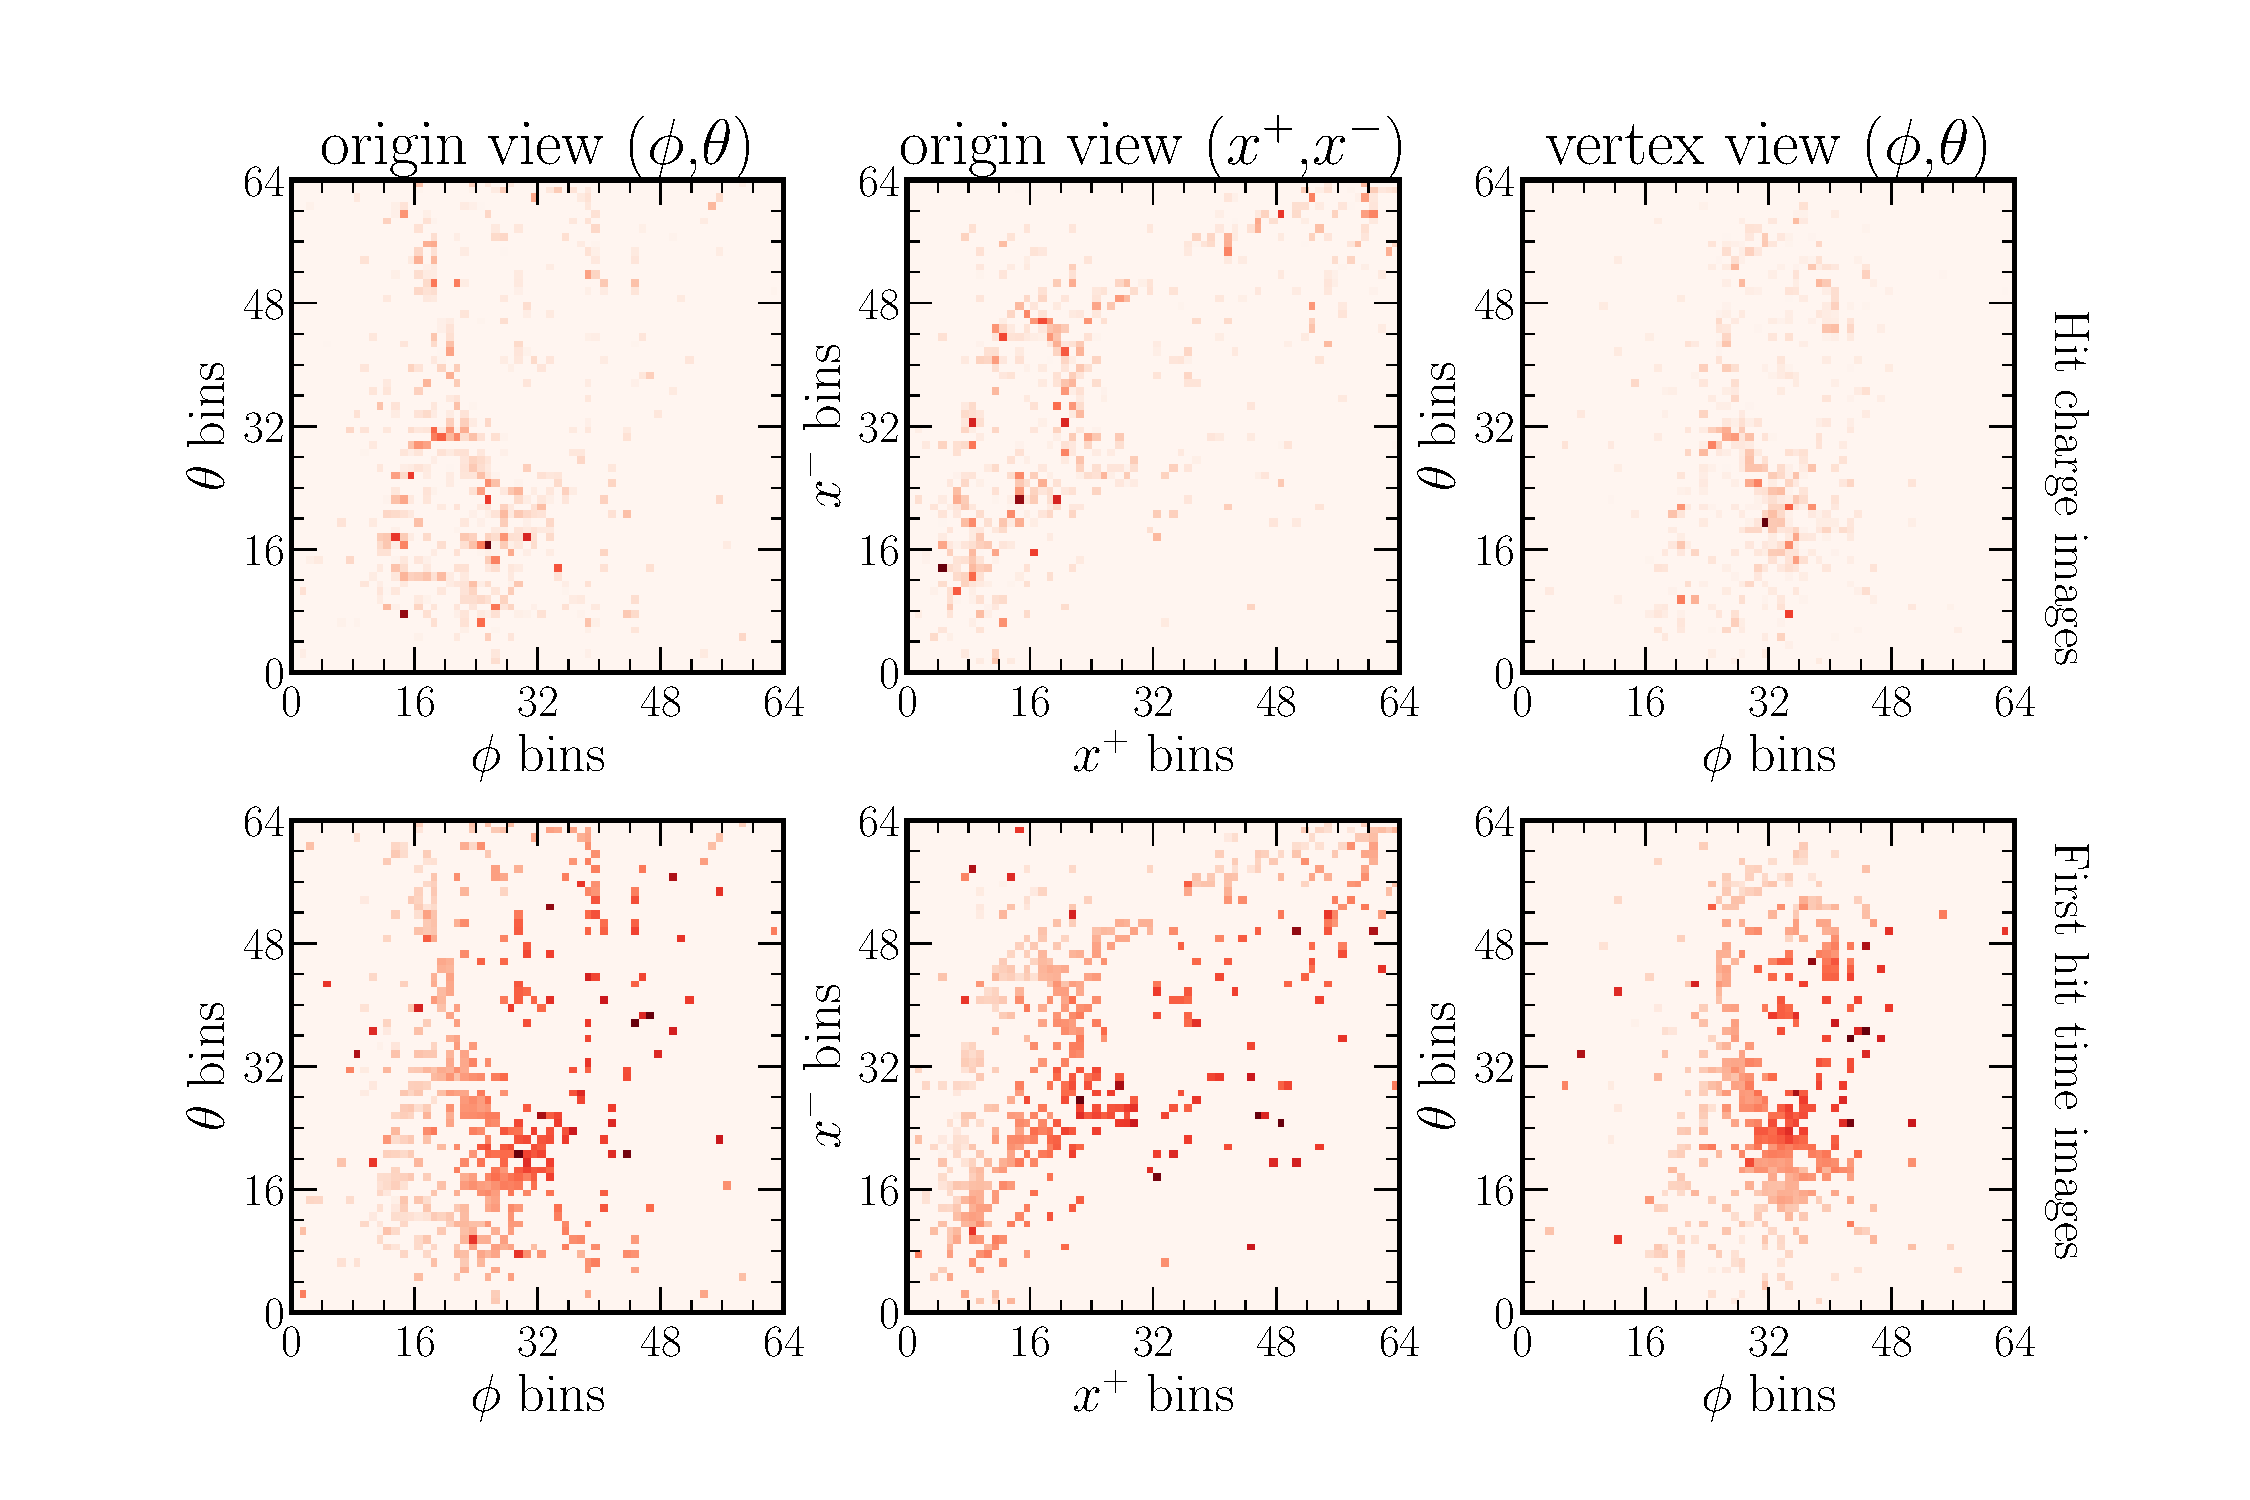
\includegraphics[width=\textwidth]{diagrams/7-cvn/chipsnet/explore_numu_ccdis_event.pdf}
    \caption[explore numu ccdis event short]
    {explore numu ccdis event long}
    \label{fig:explore_numu_ccdis_event}
\end{figure}

\begin{figure} % NUMU NCDIS EVENT DIAGRAM %
    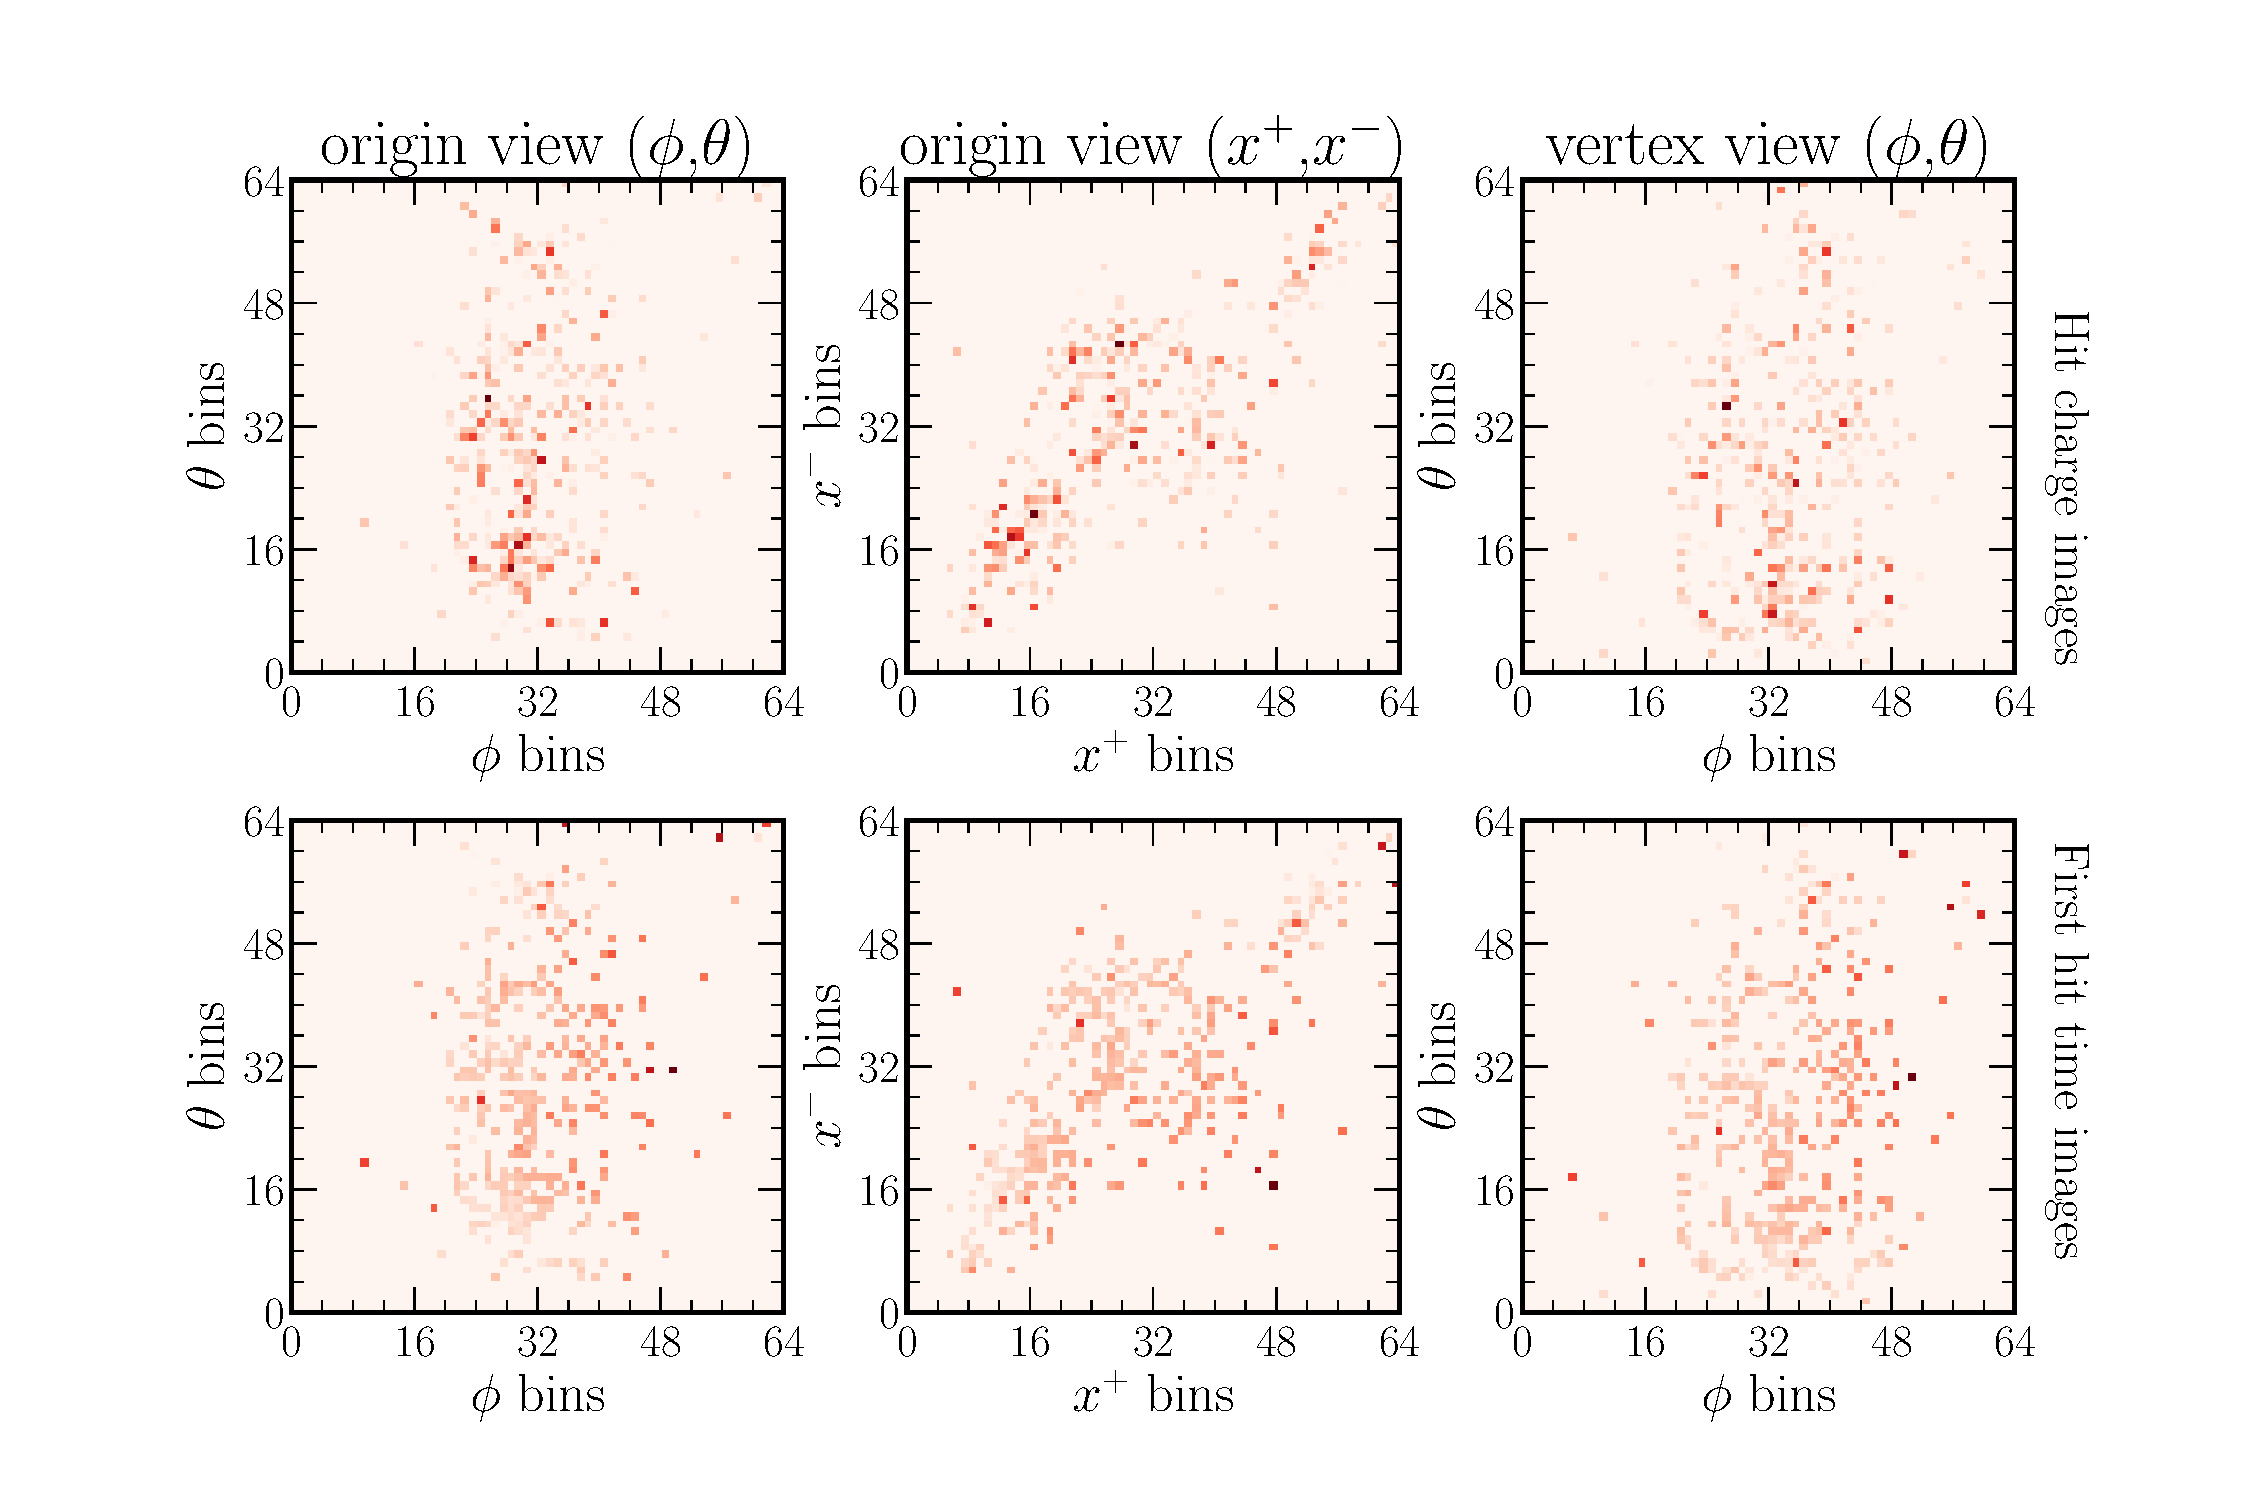
\includegraphics[width=\textwidth]{diagrams/7-cvn/chipsnet/explore_numu_ncdis_event.pdf}
    \caption[explore numu ncdis event short]
    {explore numu ncdis event long}
    \label{fig:explore_numu_ncdis_event}
\end{figure}

\begin{figure} % COSMIC MUON EVENT DIAGRAM %
    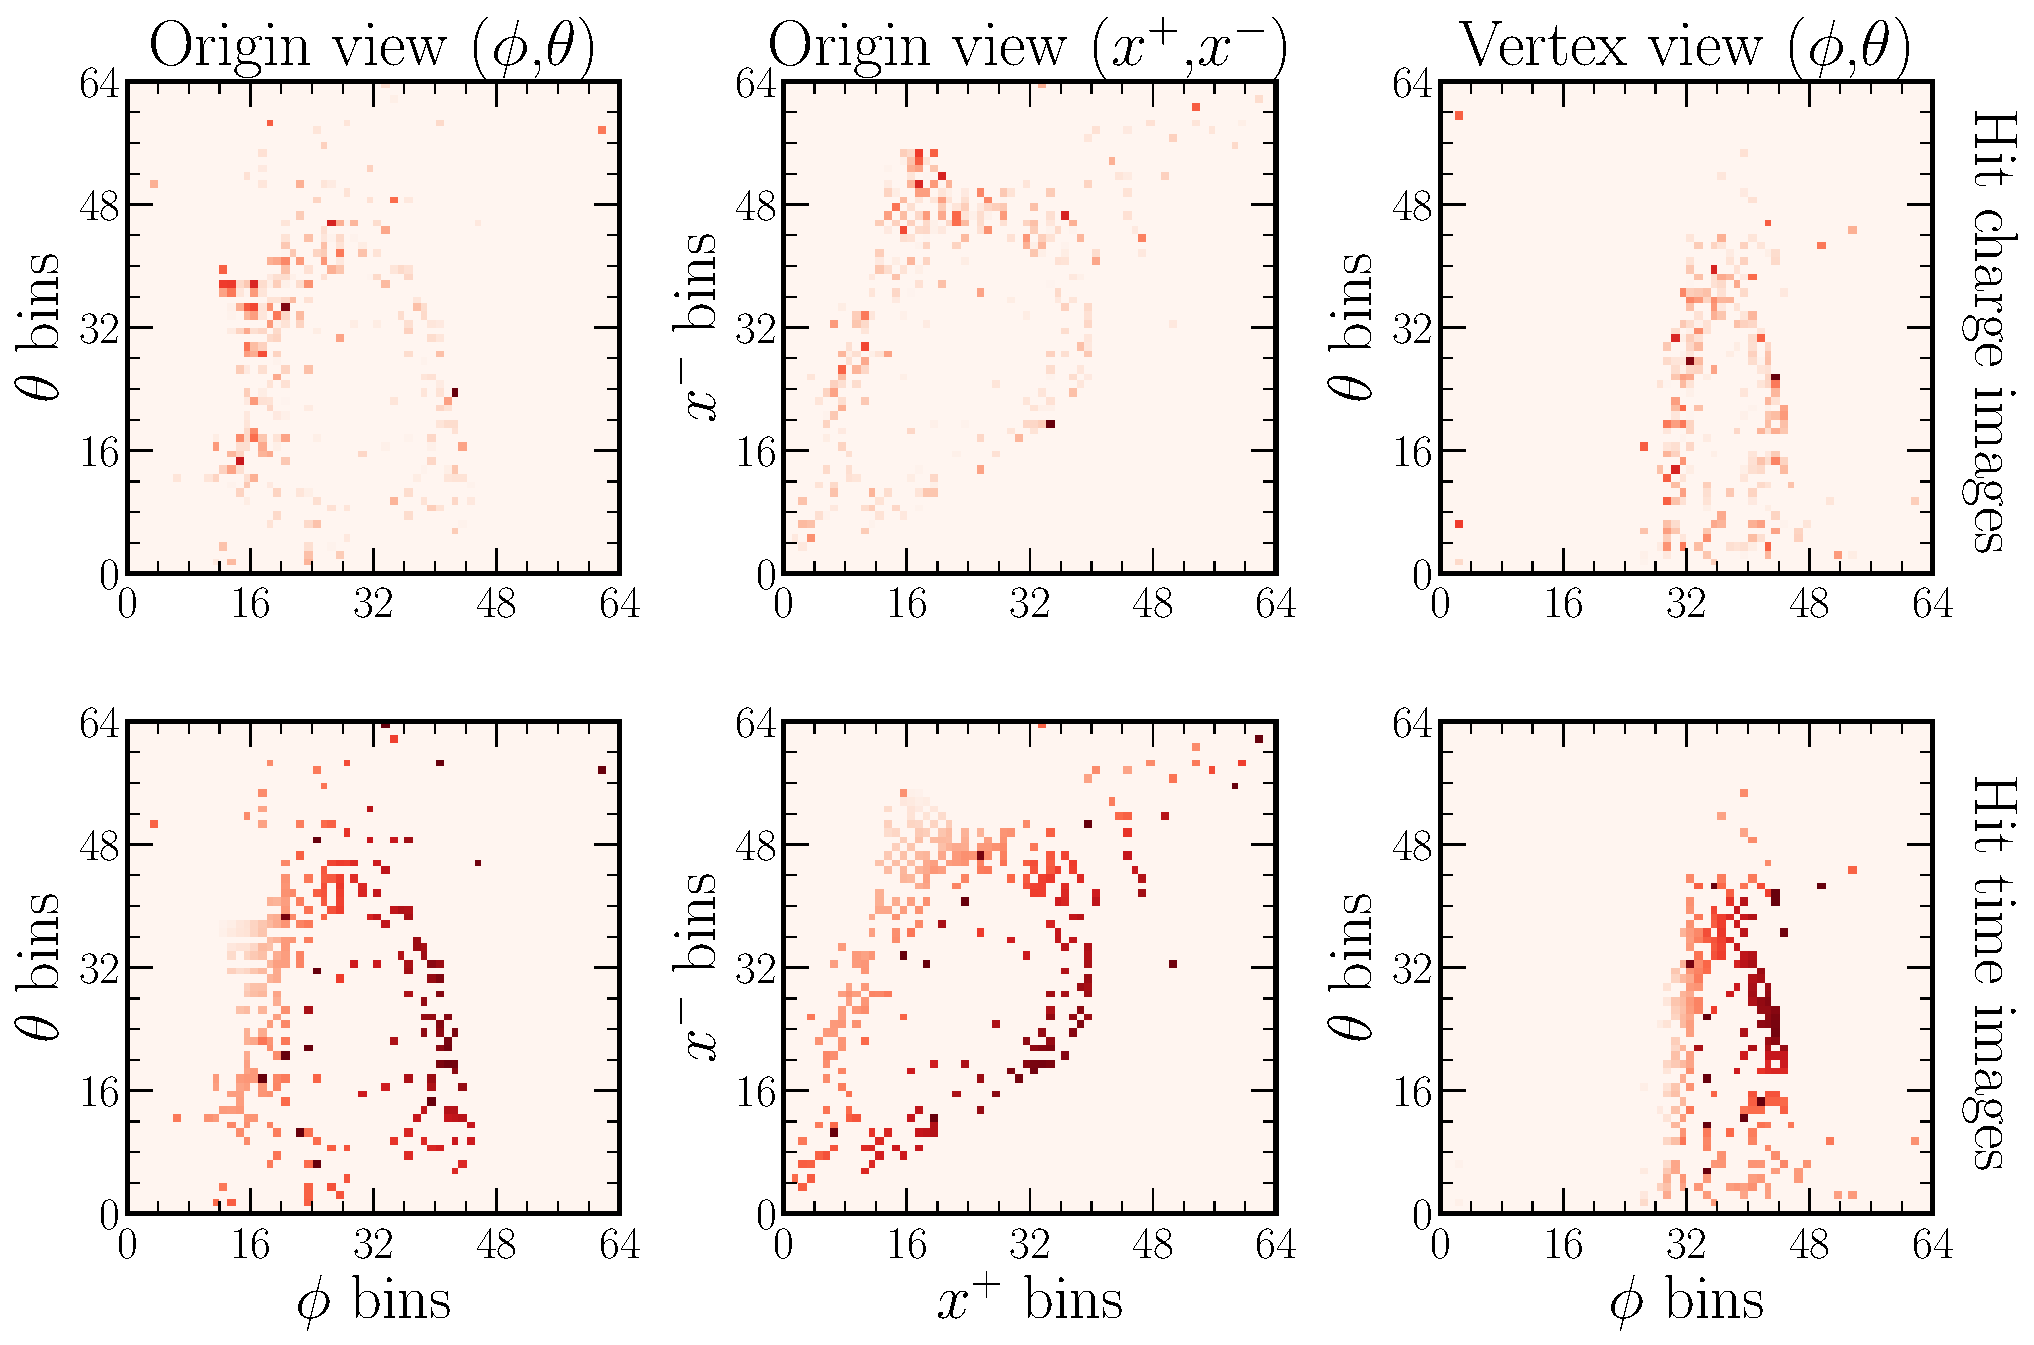
\includegraphics[width=\textwidth]{diagrams/7-cvn/chipsnet/explore_cosmic_event.pdf}
    \caption[explore cosmic event short]
    {explore cosmic event long}
    \label{fig:explore_cosmic_event}
\end{figure}

\begin{figure} % HOUGH REPRESENTATIONS DIAGRAM %
    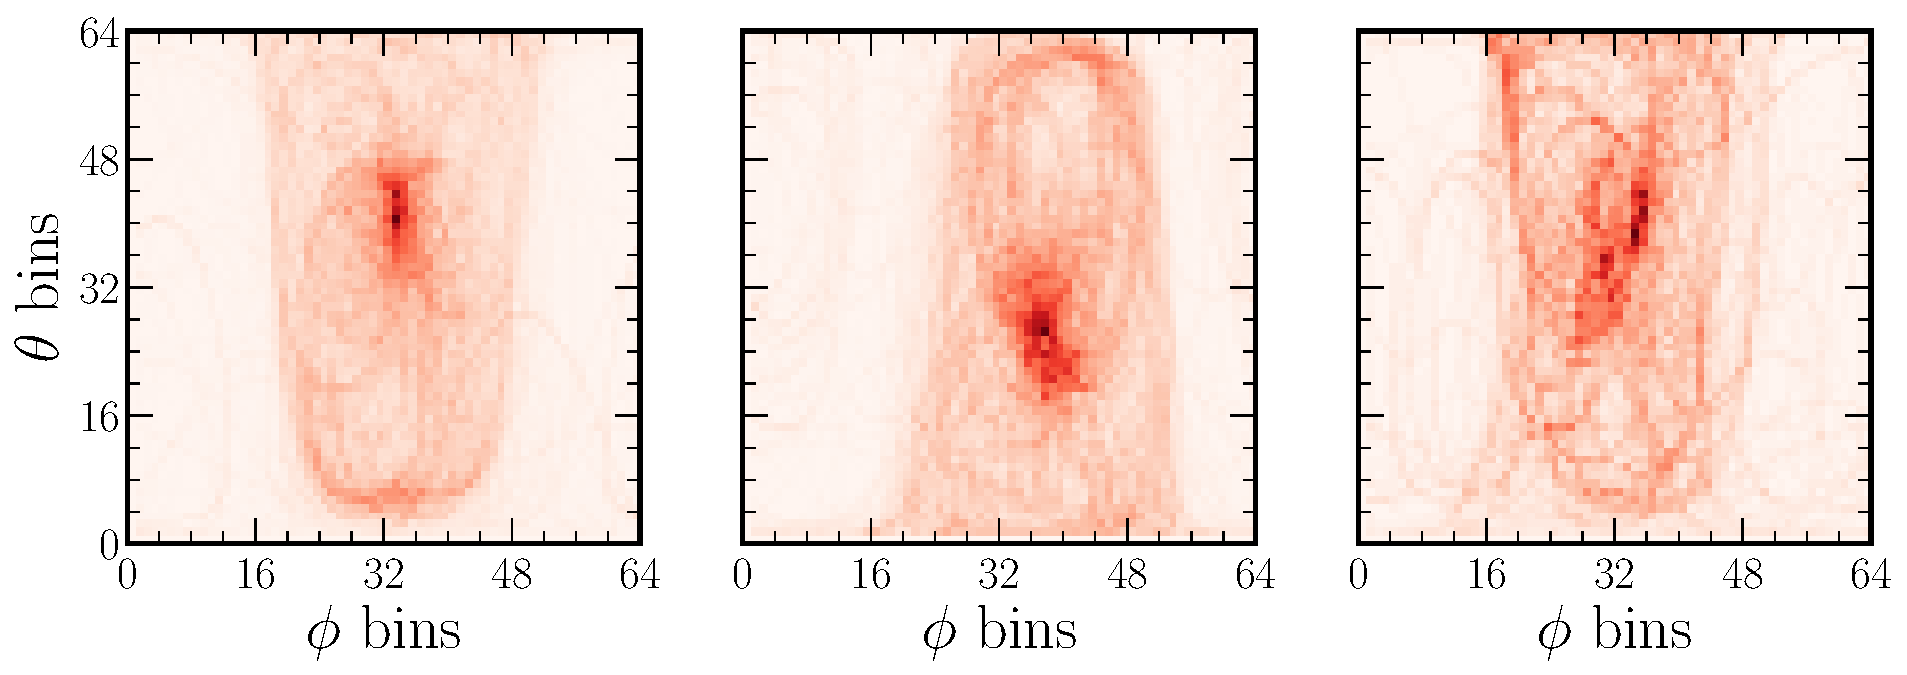
\includegraphics[width=\textwidth]{diagrams/7-cvn/chipsnet/explore_hough_events.pdf}
    \caption[example hough events short]
    {example hough events long}
    \label{fig:example_hough_events}
\end{figure}

\subsection{Multitask methodology} %%%%%%%%%%%%%%%%%%%%%%%%%%%%%%%%%%%%%%%%%%%%%%%%%%%%%%%%%%%%%%%
\label{sec:cvn_baseline_multi} %%%%%%%%%%%%%%%%%%%%%%%%%%%%%%%%%%%%%%%%%%%%%%%%%%%%%%%%%%%%%%%%%%%

Multi-task learning how to weight paper in Ref.~\cite{kendall2017}

\section{Cosmic muon rejection} %%%%%%%%%%%%%%%%%%%%%%%%%%%%%%%%%%%%%%%%%%%%%%%%%%%%%%%%%%%%%%%%%%
\label{sec:cvn_cosmic} %%%%%%%%%%%%%%%%%%%%%%%%%%%%%%%%%%%%%%%%%%%%%%%%%%%%%%%%%%%%%%%%%%%%%%%%%%%

\section{Beam classification} %%%%%%%%%%%%%%%%%%%%%%%%%%%%%%%%%%%%%%%%%%%%%%%%%%%%%%%%%%%%%%%%%%%%
\label{sec:cvn_beam} %%%%%%%%%%%%%%%%%%%%%%%%%%%%%%%%%%%%%%%%%%%%%%%%%%%%%%%%%%%%%%%%%%%%%%%%%%%%%

\section{Energy estimation} %%%%%%%%%%%%%%%%%%%%%%%%%%%%%%%%%%%%%%%%%%%%%%%%%%%%%%%%%%%%%%%%%%%%%%
\label{sec:cvn_energy} %%%%%%%%%%%%%%%%%%%%%%%%%%%%%%%%%%%%%%%%%%%%%%%%%%%%%%%%%%%%%%%%%%%%%%%%%%%

\section{Combined performance} %%%%%%%%%%%%%%%%%%%%%%%%%%%%%%%%%%%%%%%%%%%%%%%%%%%%%%%%%%%%%%%%%%%
\label{sec:cvn_final} %%%%%%%%%%%%%%%%%%%%%%%%%%%%%%%%%%%%%%%%%%%%%%%%%%%%%%%%%%%%%%%%%%%%%%%%%%%%

\section{Explainability} %%%%%%%%%%%%%%%%%%%%%%%%%%%%%%%%%%%%%%%%%%%%%%%%%%%%%%%%%%%%%%%%%%%%%%%%%
\label{sec:cvn_explain} %%%%%%%%%%%%%%%%%%%%%%%%%%%%%%%%%%%%%%%%%%%%%%%%%%%%%%%%%%%%%%%%%%%%%%%%%%

DIAGRAM: Activation plots

Initial CNN visualisation paper in Ref.~\cite{zeiler2013}
Original t-SNE paper in Ref.~\cite{maaten2008}
Grad-CAM paper in Ref.~\cite{elvaraju2019}

- For all the t-SNE stuff
- There have been plently of attempts at visualising high-dimensional data on a 2/3 dimensional
map, including Sammon mapping, Isomap, Locally Linear Embedding, Stochastic Neighbour Embedding.
- Older implementations tended to cluster all data points towards the centre of the map and proved
difficult to optimise.
- You basically set a summed probability between all points in the low-dimensional space to a
summed probability between all points in the high-dimensional space.
- t-SNE uses the student-t distribution (with a heavy tail) in the low-dimensional space to
calculate the probability. This alleviates both the crowding problem and is easier to optimise.
- Optimisation uses a simple momentum term, plus two new ideas. "Early compression" which forces
map points to stay close to each other at the start of optimisation, it is then easier for
clusters to move through each other and explore all possible global organisations of the data,
this is implemented as an L2-penalty term proportional to the sum of squared distances from the
origin, this is then removed at an iteration given as input. Secondly, "Early exaggeration" which
creates tight widely seperated clusters.

\begin{figure} % COSMIC T-SNE DIAGRAM %
    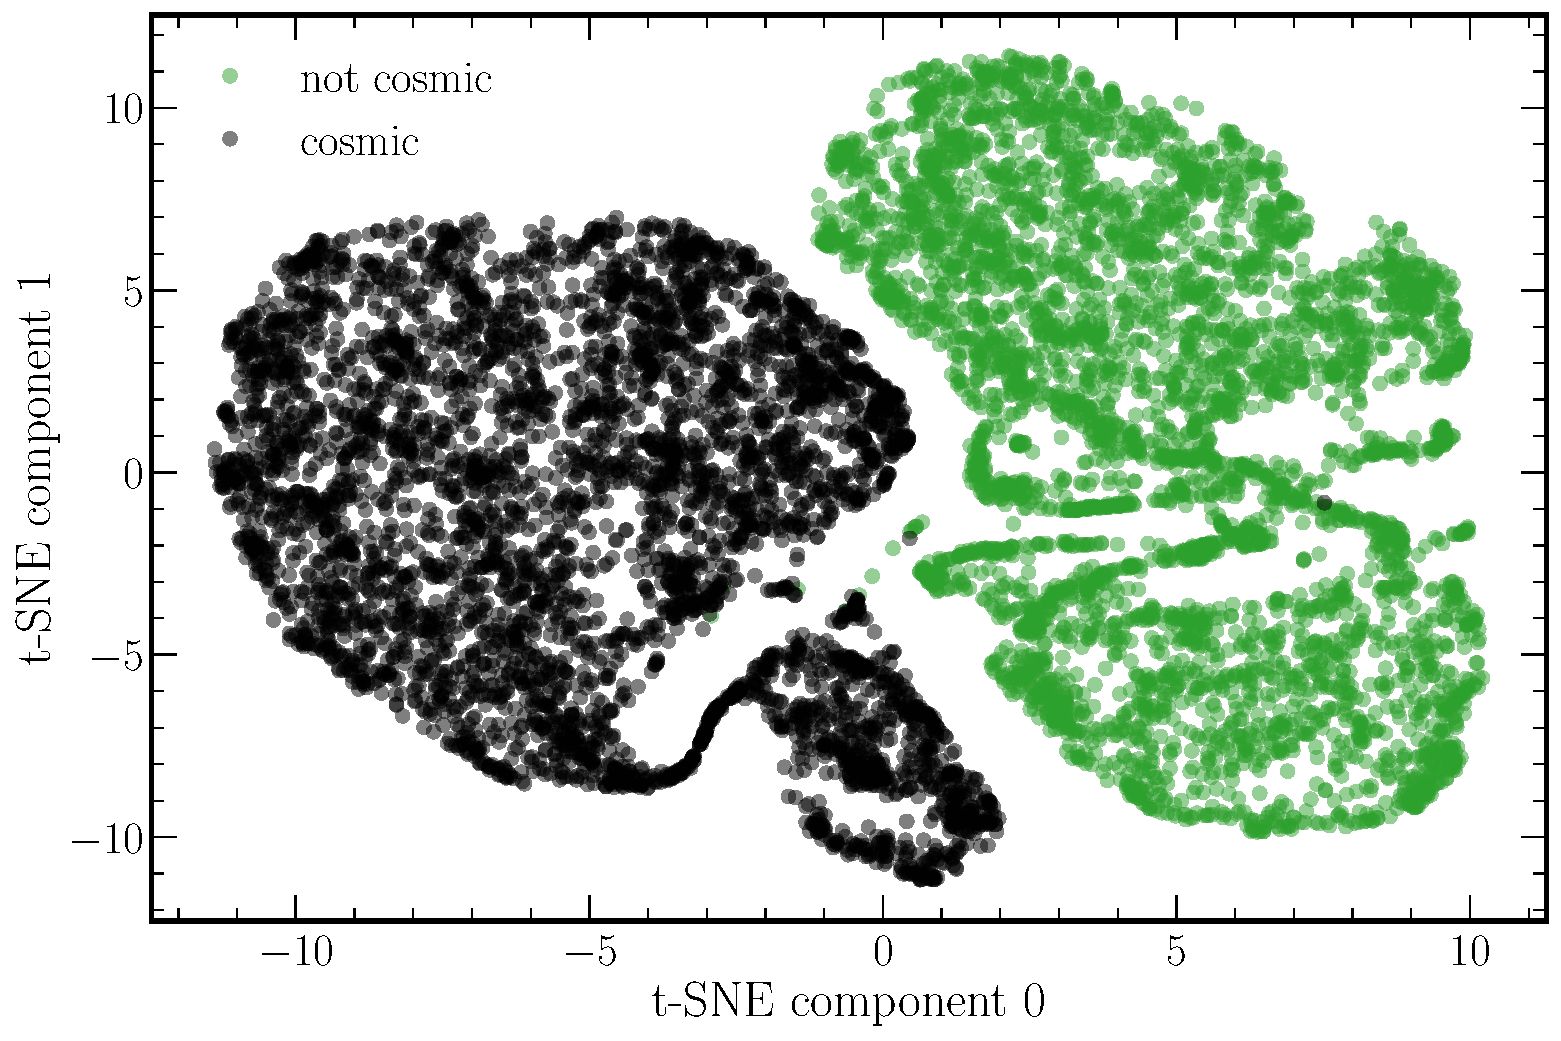
\includegraphics[width=\textwidth]{diagrams/7-cvn/chipsnet/final_cosmic_tsne.pdf}
    \caption[final cosmic tsne short]
    {final cosmic tsne long}
    \label{fig:final_cosmic_tsne}
\end{figure}

\begin{figure} % BEAM T-SNE DIAGRAM %
    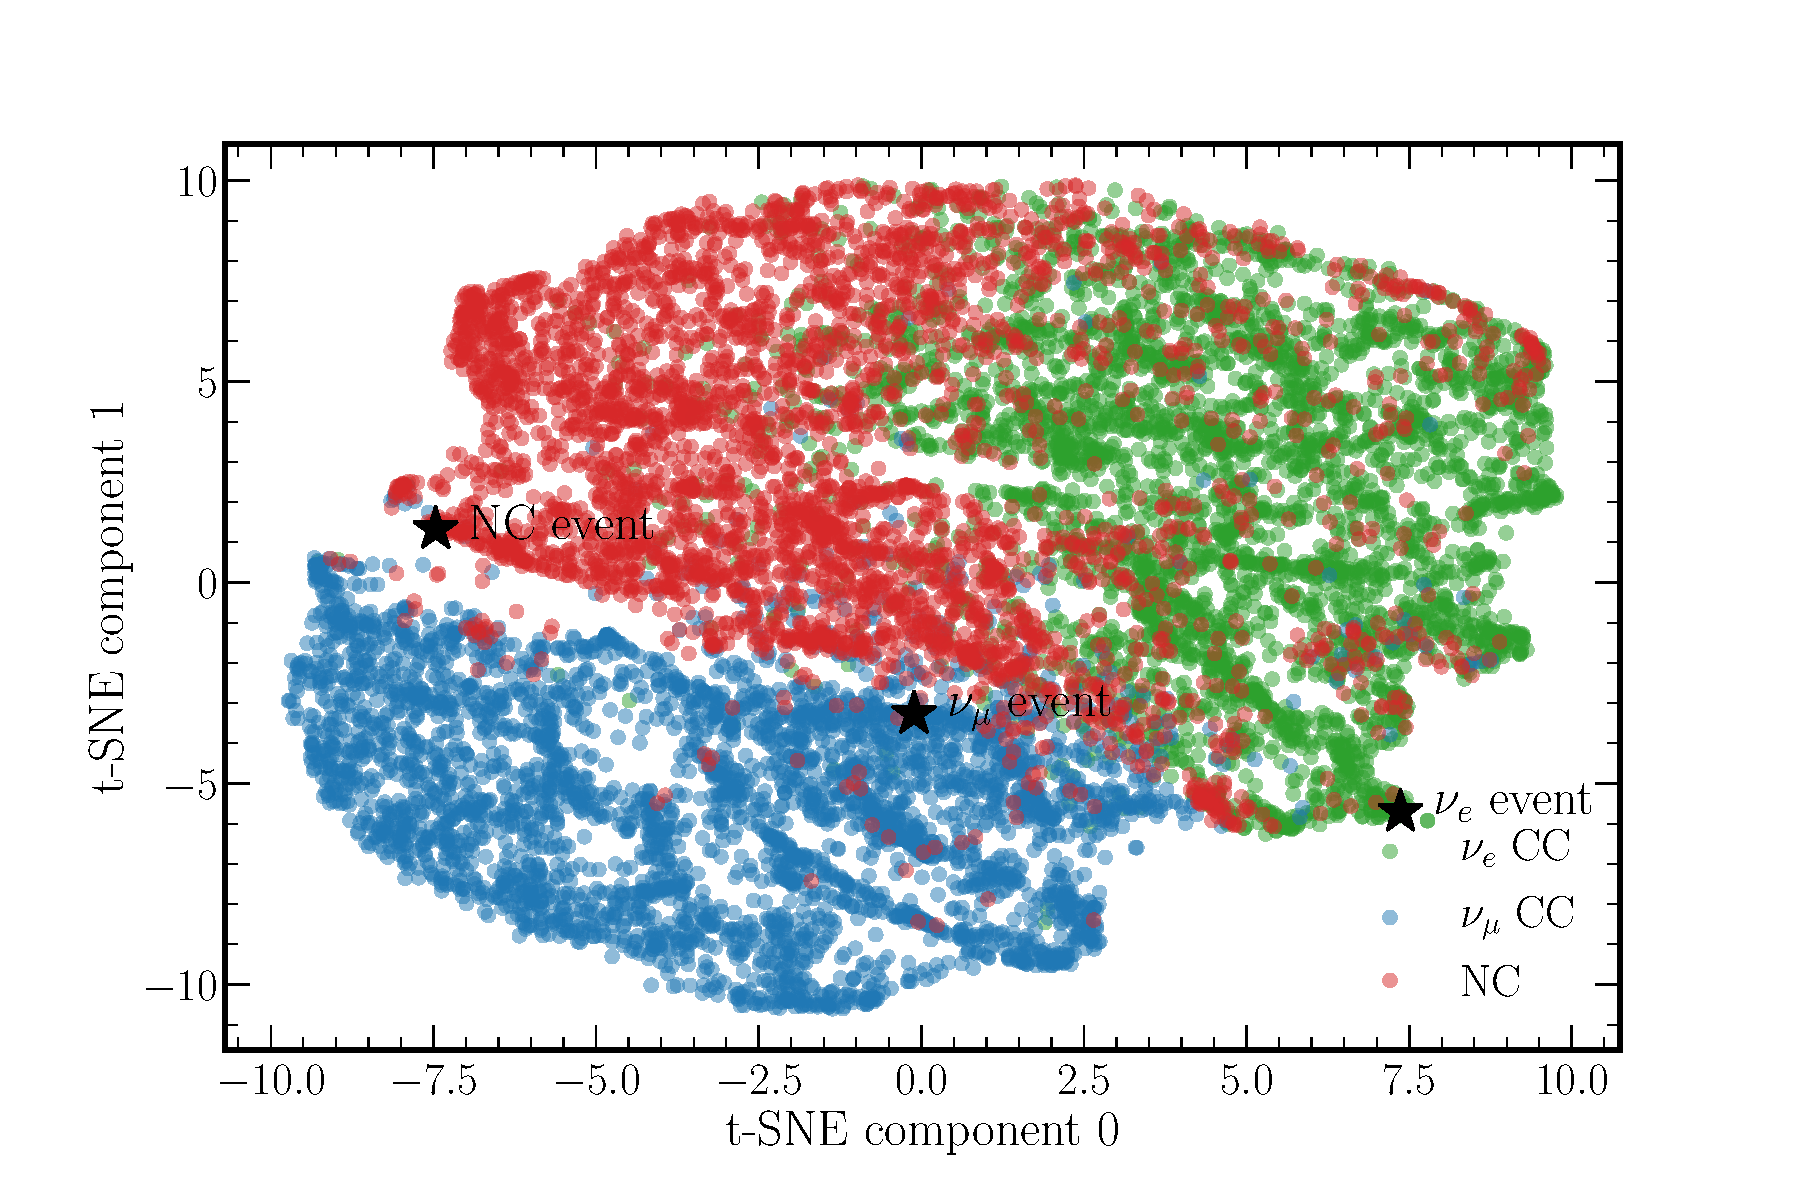
\includegraphics[width=\textwidth]{diagrams/7-cvn/chipsnet/final_beam_tsne.pdf}
    \caption[final beam tsne short]
    {final beam tsne long}
    \label{fig:final_beam_tsne}
\end{figure}

\begin{figure} % T-SNE EXAMPLE EVENTS DIAGRAM %
    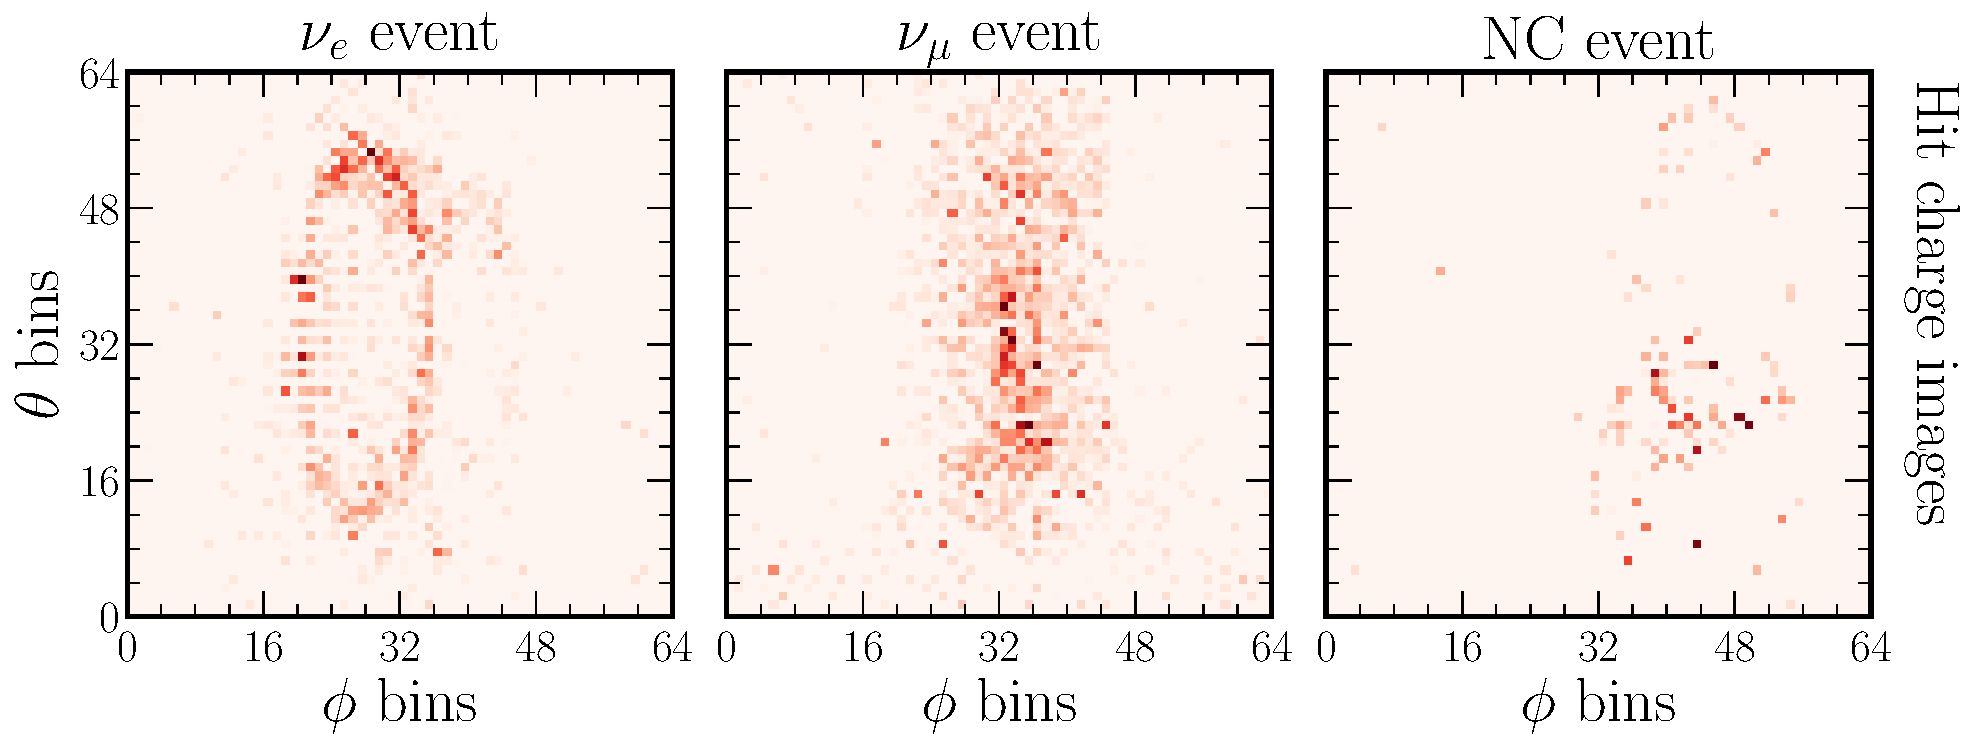
\includegraphics[width=\textwidth]{diagrams/7-cvn/chipsnet/final_beam_tsne_events.pdf}
    \caption[final beam tsne events short]
    {final beam tsne events long}
    \label{fig:final_beam_tsne_events}
\end{figure}

TODO: Sort everything below!!!!

- Take insights from neuroscience. The human eye can do remarkably well at image recognition, even neutrino event classification if
you know what to look for. But we will have way too much data, so need to train a computer to do this task for us.
- A MPL with a single hidden layer can be shown to apprximate any function arbitrarily accurately. Give REF for this.
- Conv is a set of 'filters' that when applied via scanning across an input image result in a feature map
- Pooling used as each layer requires less complexity and it is less important about the location and that the feature exists.
- Few learners search their hypothesis space fully. Therefore, a learner with a large hypothesis space that tries fewer hypotheses from it is less likely to overfit than one that tries more hypotheses from a smaller space.
- All that "deep" really means is just many many hidden layers, which can encode complex structures more efficienctly.
- They can be very difficult to train, but with GPUs, bigger training sets, weight inits, better non linearities, SGD, prevention of overfitting techniques and conv networks, its possible.

- We do not predefine the filters, they are also trained to extact the important features from the event images
- Approaches in the past for event classification using CNNs for water cherenkov detectors have taken a few Approaches to generating the input image representation.
- Projecting onto a 2d surface "outside" the detector

- Primary goal is to classify the neutrino flavour nuel CC, numu CC or NC
- Secondary goal is to then classify the individual interaction mode (QEL, RES, DIS etc...) these will have different energy resolutions and systematic uncertainties, so seperation can provide increased sensitivity.
- See signal interactions peaked closely near score values of unity and the backgrounds lie close to the zero score as expected.
- DUNE chose their selection cut to maximise the oscillation analysis sensitivity, determining sin(delta-cp) != 0
- Can choose many different output configurations/categorisations for the events.
- Should you combined into a big list of categories, should you combine the NC.
- Should you learn as seperate tasks, turns out the choice here has a decent sized impact on the final performance.
- DUne tried counting exclusive final state particles (protons, chargedpions, neutral pions)
- As the different final states will have different energy resolutions and sytematic uncertainties, it may be possible for a future analysis to improve the oscillation paramter sensitivity by indentifying subsamples with specific topologies.
- Primary partile scores can be combined to give compounded scores for the exclusive final state selections.
INFO: Need to understand the error on the number of cosmic passing the cut, is it reasonable without a huge amount of testing data?
INFO: What are the errors on all my number values? with the stats I have?
- Having a veto in the upstream towards the beam direction would be best
- Talk about how beam muons upstream of the detector are just like cosmics and say how they could be rejected aswell
INFO: proof that there is no topological difference between QEL and MEC if we are combining them for the energy stuff
- BIG UP the difference in time it takes, as this can have a huge impact on reprocessing your full dataset
- This allows a massive increase in the iteration rate of analysis, which can lead to an improved rate of improvement, with less time wasted.
- Position of PMTs does not seem to be that important

DIAGRAM: True neutrino energy distributions for different categories for energy estimation.
DIAGRAM: Neutrino energy and estimated neutrino energy distributions on same plots.
INFO: Table of the final number of expected events and efficiency and purity of the signal at the chosen cut value (nuel and numu)
DIAGRAM: Parrallel coordinates plots for tuning the hyperparameters
INFO: Time taken comparison with old reconstruction (just inference time for all stages)
DIAGRAM: Final stacked reconstructed energy distribution of selected events given a number of years running
INFO: Super-k/Dune/Nova comparison numbers for effeciencies and energy resolutions etc...
DIAGRAM: Table of how succesive cuts affect the selection of different event types
DIAGRAM: CP-Violation sensitivity from GLoBES with the new fluxes, efficiencies, smearing matrices etc... get from Tom/John
DIAGRAM: Plots of exclusive state predictions by multiplying different score outputs.

- Nova gets about ~7percent energy resolution for signal events
in Ref.~\cite{jiang2019}
- Fitqun gets ~20cm vertex position resolution for nuel CCQE events
- Fitqun gets ~16cm vertex position resolution for numu CCQE events
- Fitqun gets 5.39percent to 2.58percent lepton energy resolution for nuel CCQE events
- Fitqun gets ~2.5percent lepton energy resolution for numu CCQE events
- Note all the stuff in super-k happens at lower energies ~<1.4GeV
- In the future we could do semantic segmentation or use GANS

- CNN's have been widely applied in various computer vision tasks to solve image recongnition and analysis problems.
- The core problem in HEP is the correct categorisation of particle interactions
- This is usually done by reconstructing high-level componenets suh as clusters, tracks, showers, jets and rings. and
then summarising these objects energies, directions and shapes, these wuantities are then fed into k-nearest neighbours,
BDTs or MLPs to seperate sign from bkg.
- Prone to failure, mistakes in the reconstruction, and limitation to what has been implemented by humans.
- computer vision moved away from specifically constructed features to sing ML CNNs to discover the features.
- Manu HEP problems including water cherenkov detectors essentially result in an 'image' of an event, which are well suited to these tools.
- MLP are widely used in HEP,

- Deep neural networks have emerged as one of the most powerful supervised learning techniques.
- They truly caught the attention of the wider ML communityr in 2012 when A. Krizhevsky, I, Sutskever and G. Hinton used a GPU to train
AlexNet, lowering the error rate on the image classification task ImageNet by 12%. 
- Such was the rapid pace of advance afterwards that the ResNet model acheived a 3.57\percent error just three years later.
- Many high level libraries have now been formed, predominently led by Tensorflow (from google) and pyTorch (from facebook) making it easier to quickly code and implemenetd DNNs.
- Neural networks are neural-inspired nonlinear models for supervised learning. Constructed from the basic building blocks of a "neuron".
    \chapter{Implications for CHIPS}
\label{chap:implications}

\begin{comment}
CALIBRATION SENSITIVITY
TROUBLESOME EVENTS
PMT DISTRIBUTION
TIMING RESOLUTION
WATER QUALITY
POSSIBLE IMPROVEMENTS

- You have all of these possible parameters that can affect the performance (event categorisation
and kinematic reconstruction) of your WC detector

- Positioning of the detector (L, angle off-axis, overburden) *
- Size of the detector (height and radius) *
- Water quality (attenuation length, scattering vs absorption) *
- Which PMT’s you use (time resolution, charge collection) *
- How the PMT’s are positioned (percentage coverage, zones)
- Calibration quality (position, time, charge)
- Reconstruction methodology (likelihood vs CNN)
- Given these restrictions

- Only certain mine pits usable (fixes L and angle off-axis, use all overburden available)
- 12.5m radius for practical construction (fixes radius, but not height)
- Want to be able to carry the planes easily (Adds limits to PMT coverage percentage)
- Will just be looking at beam events, should not need much in the back
- PMT’s available. Due to cost etc… we fix the PMT’s we use, can still explore this space with
varying the time/charge. Can look at
\end{comment}
    \chapter{Summary and conclusion}
\label{chap:conclusion}

%%%%%%%%%%%%%%%%%%%%%%%%%%%%%%%%%%%%%%%%%%%%%%%%%%%%%%%%%%%%%%%%%%%%%%%%%%%%%%%%%%%%%%%%%%%%%%%%%%
%                                              PLAN                                              %
%%%%%%%%%%%%%%%%%%%%%%%%%%%%%%%%%%%%%%%%%%%%%%%%%%%%%%%%%%%%%%%%%%%%%%%%%%%%%%%%%%%%%%%%%%%%%%%%%%
\begin{comment}
TODO: Write the story of the conclusion chapter

TODO: Write the conclusion chapter section outline

TODO: Add all the sections below
\end{comment}
\end{mainmatter}

\begin{backmatter}
    %% You're recommended to use the eprint-aware biblio styles which
%% can be obtained from e.g. www.arxiv.org. The file mythesis.bib
%% is derived from the source using the SPIRES Bibtex service.
\bibliographystyle{resources/h-physrev}
\bibliography{bibliography}

%% I prefer to put these tables here rather than making the
%% front matter seemingly interminable. No-one cares, anyway!
\listoffigures
\listoftables
\end{backmatter}

\end{document} % End the document 